\documentclass[12pt,a4paper]{report}    

\usepackage[justification=centering]{caption}
\usepackage[bottom]{footmisc}
\usepackage[margin=2.5cm]{geometry}
\usepackage[hidelinks]{hyperref}
\usepackage{amssymb}
\usepackage{amsmath}
\usepackage{nccmath}
\usepackage{graphicx}
\usepackage{subcaption}
\usepackage{titlesec}
\usepackage{zref-perpage}
\usepackage[space]{grffile}
\usepackage{listings}
\usepackage{color}
\usepackage{fancyhdr}
\usepackage{fontspec}
\usepackage{setspace}
\usepackage{pdfpages}
\usepackage{float}
\usepackage{multirow}
\usepackage{array}
\usepackage[localise]{xepersian}

\settextfont[Scale=1]{IRMitra}
\setlatintextfont[Scale=.88]{Times New Roman}

\defpersianfont\titleFont[Scale=1.5]{IRMitra Bold}
\DefaultMathsDigits

\bibliographystyle{ieeetr-fa}

\titleformat*{\section}{\LARGE\bfseries}
\titleformat*{\subsection}{\large\bfseries}

\definecolor{mGreen}{rgb}{0,0.6,0}
\definecolor{mGray}{rgb}{0.5,0.5,0.5}
\definecolor{mPurple}{rgb}{0.58,0,0.82}
\definecolor{backgroundColour}{rgb}{1,1,1}

\lstdefinestyle{codeStyle}{
	backgroundcolor=\color{backgroundColour},   
	commentstyle=\color{mGreen},
	keywordstyle=\color{magenta},
	numberstyle=\tiny\color{mGray},
	stringstyle=\color{mPurple},
	basicstyle=\footnotesize,
	breakatwhitespace=false,         
	breaklines=true,                 
	captionpos=b,                    
	keepspaces=true,                 
	numbers=left,                    
	numbersep=5pt,                  
	showspaces=false,                
	showstringspaces=false,
	showtabs=false,                  
	tabsize=2
}


\renewcommand{\bibname}{مراجع}

\fancyhead[R]{\fontsize{14}{15} \selectfont ایستگاه هواشناسی دیجیتال}
\fancyhead[L]{\fontsize{14}{15} \selectfont \leftmark}

\defpersianfont{\titr}{XB Titre}

\makeatletter
\newcommand\Notefont{\LARGE}
\long\def\bibNote#1{\gdef\@bibNote{\item[]{\Notefont#1}}}
\renewenvironment{thebibliography}[1]{%
	\@xp\chapter\@xp*\@xp{\bibname}%
	\normalfont\normalsize\labelsep .5em\relax
	\renewcommand\theenumiv{\arabic{enumiv}}\let\p@enumiv\@empty
	\list{\@biblabel{\theenumiv}}{\@bibNote\settowidth\labelwidth{\@biblabel{#1}}%
		\leftmargin\labelwidth \advance\leftmargin\labelsep
		\usecounter{enumiv}}%
	\sloppy \clubpenalty\@M \widowpenalty\clubpenalty
	\sfcode`\.=\@m
}{%
	\def\@noitemerr{\@latex@warning{Empty `thebibliography' environment}}%
	\endlist
}
\makeatother

\bibNote{\section*{مراجع}}

\newcolumntype{C}[1]{>{\centering\let\newline\\\arraybackslash\hspace{0pt}}m{#1}}

\begin{document}

	\pagenumbering{harfi} \pagestyle{empty} \baselineskip1.2\baselineskip
	
	\clearpage \setcounter{page}{1}
	\includepdf[pagecommand={\thispagestyle{empty}}]{parts/bismillah.pdf}
	
	\clearpage \setcounter{page}{2}
	%!TeX root=../main.tex
\begin{titlepage}
	\begin{center}
		\includegraphics[width=0.3\textwidth]{Assets/logo.pdf}\\
		\smallskip \LARGE
		{دانشگاه دامغان}\\
		{دانشکده فنی و مهندسی}\\
		
		\vspace{1cm} \LARGE
		\textbf{گزارش پروژه کارشناسی\\مهندسی برق}\\
		
		\vspace{1cm}
		
		\huge
		\textbf{ایستگاه هواشناسی دیجیتال}
		
		\LARGE
		\vspace{3cm}
		{دانشجویان}\\
		\vspace{0.25cm}
		\textbf{مهدی جمشیدی\\محمدابراهیم ابراهیم‌طوسی}\\
		
		\vspace{1.2cm}
		{استاد راهنما}\\
		\vspace{0.25cm}
		\textbf{دکتر بهزاد بقراطی}
		
		\vfill
		{1399}
	\end{center}
\end{titlepage}
	
	\clearpage \setcounter{page}{3}
	\includepdf[pagecommand={\thispagestyle{empty}},pages=-]{parts/confirmation.pdf}
	\clearpage 
	\doublespacing
	\fontsize{16}{17}\selectfont
	
	\setcounter{page}{6}
	
	%!TeX root=../main.tex
\clearpage
\pagestyle{empty}
\vspace*{\fill}

\section*{چکیده}

محور اصلی پروژه، طراحی و پیاده‌سازی ایستگاه هواشناسی سینوپتیک (\متن‌لاتین{Synoptic}) متشکل از یک دستگاه که در فاصله چند کیلومتری از مرکز اصلی قرار داده می‌شود تا پارامترهای جوی نظیر دمای هوا، فشار، رطوبت، شدت نور، سرعت و جهت باد را اندازه‌گیری کرده و داده‌ها را از طریق امواج رادیویی به دستگاه دیگر که در پایگاه قرار دارد جهت ثبت و نمایش روی رایانه‌های پایگاه مخابره کند، می‌باشد. در این پروژه از میکروکنترلر \متن‌لاتین{STM32} جهت برنامه‌ریزی و ایجاد ارتباط میان بخش‌های مختلف و همچنین از گیرنده و فرستنده‌های آلتراسونیک جهت محاسبه سرعت و جهت باد استفاده‌شده است. به‌طورکلی با استفاده از سنسورهای دیجیتال در این پروژه علاوه بر کم‌تر شدن حجم دستگاه‌ها مصرف انرژی آن نیز نسبت به ایستگاه‌های سنتی که تجهیزاتی اغلب مکانیکی داشتند کمتر شده است. درنهایت نیز استفاده از ماژول لورا (\متن‌لاتین{LoRa}) به‌عنوان بهینه‌ترین و کم‌هزینه‌ترین روش ارتباط راه گشای انتخاب روش ارسال داده‌های رادیویی خواهدبود. 

\noindent
{\bf
واژه‌های كليدی:
} 
\متن‌لاتین{STM32}، \متن‌لاتین{LoRa}، \متن‌لاتین{Ultrasonic}، \متن‌لاتین{Python}

\vspace*{\fill}
\clearpage
	
	\pagestyle{plain} \setcounter{page}{1} \pagenumbering{tartibi} 
	
	\tableofcontents
	
	\newpage \setcounter{page}{0} \pagenumbering{arabic} \setcounter{page}{1} \baselineskip1.1\baselineskip 
	\zmakeperpage{footnote}
	\titleformat{\chapter}[display]{\vfill\filcenter\bfseries}{\titr\raggedleft\fontsize{36}{38}\selectfont\chaptername~\thechapter}{10ex}{\titr\fontsize{36}{38}\selectfont}
	[\vfill\vfill\vfill\null\thispagestyle{empty}\clearpage\newpage\vspace*{6\baselineskip}]
	\titlespacing{\chapter}{0pt}{0ex}{0ex}
	
	\pagestyle{fancy}
	
	\fontsize{15}{16}\selectfont
	
	%!TeX root=../main.tex
\فصل{مقدمه}
\begingroup

\titleformat{\section}[display]{\normalfont\huge\bfseries}{}{0pt}{}

\قسمت{مقدمه}

ایستگاه هواشناسی، مرکزی مجهز به تجهیزات و ابزارهایی برای اندازه‌گیری‌های جوی است که به ارائه اطلاعات برای پیش‌بینی و مطالعه آب‌وهوا می‌پردازد. اندازه‌گیری انجام‌شده معمولاً شامل دما، فشار هوا، رطوبت، سرعت باد، جهت باد و مقدار بارش است. مشاهدات دستی حداقل یک بار در روز انجام می‌شود، درحالی‌که اندازه‌گیری خودکار حداقل یک بار در ساعت انجام می‌پذیرد.

ایستگاه‌های هواشناسی معمولی مجهز به ابزارهای زیر هستند \مرجع{wikipedia:Weather_station}:

\شروع{فقرات}
\فقره
رطوبت‌سنج برای اندازه‌گیری رطوبت
\فقره
فشارسنج برای اندازه‌گیری فشار جو
\فقره 
دماسنج برای اندازه‌گیری دمای هوا
\فقره
پیرانومتر برای اندازه‌گیری تشعشعات خورشیدی
\فقره
باران‌سنج برای اندازه‌گیری میزان بارش باران در طی یک دوره زمانی مشخص
\فقره
تجهیزاتی نظیر بادسنج، پرچم باد یا جوراب باد برای اندازه‌گیری سرعت و جهت باد
\پایان{فقرات}

ایستگاه‌های پیشرفته‌تر همچنین ممکن است شاخص فرابنفش، رطوبت برگ، رطوبت خاک، دمای خاک، دمای آب در حوضچه‌ها، دریاچه‌ها، نهرها یا رودخانه‌ها و گاهی داده‌های دیگر را اندازه‌گیری کنند. به‌جز دستگاه‌هایی که نیازمند تماس مستقیم با عناصر مورداندازه‌گیری هستند (نظیر بادسنج)، دیگر سنسورها و دستگاه‌ها باید در محفظه‌ای به‌دوراز تابش مستقیم خورشید و وزش باد قرار بگیرند.

ایستگاه‌های هواشناسی سینوپتیک (\متن‌لاتین{Synoptic}) 24 ساعته به‌صورت خودکار هر سه ساعت به سه ساعت پارامترهای جوی را پس از اندازه‌گیری و جمع‌آوری از طریق شبکه‌های مخابراتی منتقل می‌کنند. به‌طور مشابه ایستگاه‌هایی با نام متار (\متن‌لاتین{Metar}) این کار را هر  یک ساعت انجام می‌دهند. وظیفه این ایستگاه‌ها جمع‌آوری اطلاعات جوی از محدوده‌هایی وسیع و مخابره به ایستگاه‌های اصلی به‌منظور اطلاع از وضعیت حال و گذشته و پیش‌بینی شرایط آب و هوایی مناطق در آینده است. 

هدف این پروژه پیاده‌سازی نوعی ایستگاه هواشناسی سینوپتیک است که با تجهیزات ارزان و کم‌مصرف دیجیتالی پارامترهای جوی لازم را جمع‌آوری و به‌صورت بی‌سیم به ایستگاهی جهت ثبت و نمایش مخابره می‌کند. در این پروژه از میکروکنترلر (\متن‌لاتین{Microcontroller}) \متن‌لاتین{ARM} سری \متن‌لاتین{STM32F10X} به‌عنوان هسته اصلی پردازش در هر دو سمت سنسور و ایستگاه و از ماژول لورا (\متن‌لاتین{LoRa}) با چیپ \متن‌لاتین{SX1278} به‌منظور برقراری ارتباط بی‌سیم استفاده شده ‌است.

\endgroup
	
	%!TeX root=../main.tex
\فصل{آشنایی با میکروکنترلرهای \متن‌لاتین{ARM} و نرم‌‌افزار \متن‌لاتین{STM32CubeIDE}}
\قسمت{مقدمه}
\begin{figure}[!h]
	\centering
	\includegraphics[width=0.7\linewidth]{Assets/arm.png}
\end{figure}

\متن‌لاتین{ARM} یک شرکت بریتانیایی و چندملیتی است که در زمینه نیمه‌‌رساناها و طراحی نرم‌افزارهای رایانه‌ای فعالیت می‌کند. نحوه تجارت این شرکت به این صورت است که گواهی‌نامه محصولات خود را به عنوان \متن‌لاتین{IP Core} به فروش می‌رساند و شرکت‌های دیگر از جملهNXP,  \متن‌لاتین{ST} \متن‌لاتین{Microelectronics}, \متن‌لاتین{Qualcomm}, \متن‌لاتین{Texas Xilinx}, \متن‌لاتین{Nvidia}, \متن‌لاتین{Atmel}, \متن‌لاتین{Apple} این لایسنس را خریداری کرده و محصولات خود را بر اساس آن تولید می‌کنند.

\قسمت{معماری \متن‌لاتین{ARM}}
معماری آرم\پانویس{ARM}، نوعی از معماری 32 بیتی و 64 بیتی، بر طبق طراحی \متن‌لاتین{RISC CPU} و ساختار پردازنده‌های رایانه‌ای است که به‌وسیله شرکت انگلیسی آرم هولدینگز\پانویس{Arm Holdings} طراحی شده‌است و به دلیل قیمت ارزان، سرعت بسیار زیاد، سخت‌‌افزارهای جانبی متعدد از جمله: \متن‌لاتین{CAN}, \متن‌لاتین{Ethernet}, \متن‌لاتین{UART}, \متن‌لاتین{SPI}, \متن‌لاتین{USB}, \متن‌لاتین{DAC}, \متن‌لاتین{ADC}, \متن‌لاتین{SDRam} و غیره، حافظه داخلی زیاد و توان مصرفی پایین (به ازای هر \متن‌لاتین{MHz}، جریانی از 0٫2 میلی‌آمپر تا 1 میلی آمپر مصرف می کنند). این پردازنده ها؛ اکثر سیستم های نهفته (مثل میکروکنترلرها، موبایل و تبلت و کلا سیستم هایی با حجم کوچک و امکانات بالا) از این پردازنده استفاده می کنند. معماری آرم از دهه ۱۹۸۰ میلادی تا به امروز در حال توسعه و گسترش است. \متن‌لاتین{ARM} مخفف \متن‌لاتین{Advanced RISC Machine} است و از آنجایی که این معماری براساس طراحی \متن‌لاتین{RISC} بنا شده‌‌است، برای هسته اصلی پردازشگر تنها به حدود ۳۵ هزار ترانزیستور نیاز است و این باعث می‌شود که پردازنده بسیار کم‌مصرف شود، کم‌تر داغ کند و نیازی به خنک‌کننده یا فن نداشته باشد بر خلاف معماری x86 به‌کار رفته در پردازنده‌های شرکت‌های اینتل و ای‌ام‌دی که نیازمند میلیون‌ها ترانزیستور هستند و همین مسئله باعث افزایش توان مصرفی و داغ شدن آنان می‌شود. شرکت آرم هولدینگز در سال ۲۰۱۴ معماری آرم با قابلیت پشتیبانی از دستورالعمل‌های ۶۴ بیتی در پردازنده‌های کورتکس-ای۵۳ و کورتکس-ای۵۷ توسط این شرکت تولید و عرضه شد.
از میان شرکت‌هایی که تولیدکننده میکروکنترلرهای 32بیتی هستند؛ میکروکترلرهای کمپانی \متن‌لاتین{ST} بیشترین محبوبیت را در صنعت دارد که قیمت پایین و در حین حال امکانات بالا و منابع اموزشی کامل از مزایای آن هستند.

\قسمت{میکروکنترلرهای شرکت ST}
\begin{figure}[!h]
	\centering
	\includegraphics[width=0.7\linewidth]{Assets/stm.png}
\end{figure}
\زیرقسمت{مقدمه}
اس‌تی‌ام‌الکترونیکس، شرکت فرانسوی-ایتالیایی و چندملیتی تولیدکننده تجهیزات الکترونیکی و نیمه‌هادی‌ها می‌باشد، که دفتر مرکزی آن در شهر ژنو، سوئیس قرار دارد. این شرکت بر پایه میزان درآمد، به عنوان بزرگترین سازنده تراشههای نیم‌رساناها در اروپا محسوب می‌شود. در حالی که دفتر مرکزی شرکت اس‌تی‌میکروالکترونیکز و ستاد مدیریتی آن، در ژنو قرار گرفته‌است، ولی بخش عملیاتی این شرکت، در شهر آمستردام، هلند مستقر می‌باشد. دفتر مرکزی شعبه ایالات متحده این شرکت، در شهر کاپل، تگزاس قرار دارد. ستاد مرکزی شعبه آسیا اس‌تی‌میکروالکترونیکز در سنگاپور و ساختمان مرکزی شعبه ژاپن و کره جنوبی آن نیز، در توکیو مستقر می‌باشند. دفتر مرکزی شعبه چین این شرکت، در شهر شانگهای قرار گرفته‌است. شرکت اس‌تی‌مایکروالکترونیکس، در فهرست اولیه بازار بورس یورونکست ذکر شده‌است و به عنوان جزئی از شاخص فرانسوی کاک ۴۰ محسوب می‌شود. این شرکت همچنین در فهرست ثانویه از بازار بورس نیویورک و نیز بازار بورس ایتالیا، ذکر شده‌است.

\زیرقسمت{نحوه نام‌گذاری}
\begin{figure}[!h]
	\centering
	\includegraphics[width=\linewidth]{Assets/stmnaming.png}
	\caption{جدول نحوه نام‌گذاری میکروکنترلرهای شرکت \متن‌لاتین{ST}.}
	\label{fig:stmnaming}
\end{figure}

نام‌گذاری این میکروکنترلرها همواره با عبارت \متن‌لاتین{ST} شروع می‌شود که معرف شرکت سازنده خود می‌باشد. بعد از ترکیب \متن‌لاتین{ST} حرف \متن‌لاتین{M} می‌آید که نشانگر این است که محصول حاضر یک میکروکنترلر می‌باشد. بعد از \متن‌لاتین{STM} یکی از عبارات $32$، $8$ یا $8A$ را خواهیم دید که به ترتیب معرف میکروهای ۳۲بیتی، ۸بیتی و ۸بیتی \متن‌لاتین{Automotive} می‌باشد. تا این مرحله خانواده کلی محصول مورد نظر معرفی گردید و سپس نوبت به تشریح ویژگی‌های میکروکنترلر می‌رشد. کاراکتر بعدی در نام‌گذاری فقط شامل یک حرف انگلیسی می‌باشد و یکی از حروف F ،L ،P ،S ،T یا W است. این حروف نوع محصول را مشخص می‌کنند. به طور مختصر باید گفت که حرف F مربوط به محصولات \متن‌لاتین{Foundation}، حرف L مربوط به \متن‌لاتین{Ultra-low power}، حرف P محصولات \متن‌لاتین{Pre-programmed}، حروف S مختص \متن‌لاتین{Standard}، عبارت T برای \متن‌لاتین{Touch sensing} و در نهایت W برای معرفی محصولات \متن‌لاتین{Wireless} به کار می‌روند. سپس شاهد یک عدد سه رقمی خواهیم بود. این عدد (مخصوصا رقم سوم) با حرف قبلی در ارتباط است.  این عدد ویژگی‌های خاص هر خانواده میکروکنترلر رو نشان می‌دهد، از جمله معماری، طبقه‌بندی، حداکثر فرکانس، حداکثر حافظه \متن‌لاتین{SRAM} و حداکثر حافظه \متن‌لاتین{Flash}. به عنوان مثال عدد 103 در میکروکنترلرهای \متن‌لاتین{STM32F103} نشانگر این می‌باشد که معماری این میکرو \متن‌لاتین{Cortex-M3} در طبقه‌بندی \متن‌لاتین{Mainstream} با حداکثر فرکانس 72 مگاهرتز، حداکثر حافظه فلش ۱۰۲۴ کیلوبایتی و حداکثر حافظه اِس-رم ۹۶ کیلوبایتی می‌باشد. لازم به ذکر است این اعداد منحصر بفرد می‌باشد و تقریبا الگوی مشخصی ندارد. در این عدد رقم سوم (رقم صدگان) از اهمیت بیشتری برخوردار هستش و اطلاعات اصلی را همین رقم بیان می‌کند. بعد از این عدد دوباره شاهد یک حرف انگلیسی خواهیم بود. این حرف تعداد پین‌های میکروکنترلر مورد نظر را مشخص می‌کند. بعد از آن، یک عدد یا حرف می‌بینیم که بیانگر مقدار حافظه \متن‌لاتین{Flash} میکروکنترلر می‌باشد. توجه داشته باشید که عدد ۳ رقمی قبل مقدار حداکثری حافظه \متن‌لاتین{Flash} خانواده را مشخص می‌کرد ولی عدد یا حرف حاضر دقیقا مقدار این حافظه را در این میکروکنترلر برای ما بازگو می‌کند. بعد از این قسمت دوباره شاهد یک حرف انگلیسی خواهیم بود که برای ما مشخص می‌کند میکروکنترلر مورد بحث از چه نوع پکیجی برخوردار است و در نهایت باز شاهد یک عدد یا حرف انگلیسی خواهیم بود که مشخص کننده رنج دمای کاری میکروکنترلر مربوطه می‌باشد. به این صورت که A یا ۶ محدوده ۴۰- تا ۸۰ درجه سانتی‌گراد، B یا ۷ محدوده ۴۰- تا ۱۰۵ درجه، C یا ۳ محدوده ۴۰- تا ۱۲۵ درجه و D محدوده ۴۰- تا ۱۵۰ درجه را مشخص می‌کند. مطالب بیان شده به صورت کلی در شکل \رجوع{fig:stmnaming} قابل مشاهده است.

\زیرقسمت{انواع کتابخانه‌های مورد استفاده در میکروکنترلرهای ST}
\زیرزیرقسمت{CMSIS}
یک لایه نرم‌افزاری برای سخت‌افزار پردازنده‌های کورتکس M هست که توسط بنیاد \متن‌لاتین{ARM}، تعریف‌شده و فارغ از شرکت سازنده میکروکنترلر است. به عبارتی \متن‌لاتین{CMSIS} ارائه‌شده برای شرکتی چون \متن‌لاتین{ST} مشابه همان CMSISای است که برای شرکت فیلیپس یا شرکت‌های دیگر ارائه شده. این یکسان بودن موجب می‌شود تا اصطلاحاً \متن‌لاتین{Portability} برنامه نوشته شده، بالا رود.
درواقع شما به کمک \متن‌لاتین{CMSIS} یک‌بار برای میکرویی کد می‎‌زنید و با کمترین تغییرات ممکن، می‌توانید آن را بر روی میکرویی از شرکتی دیگر انتقال دهید. این لایه بیشتر از آنکه حاوی توابعی برای انجام کارهای مختلف با پریفرال‎‌های میکرو باشد، دارای تعریف‌های1 مختلف از رجیسترهای میکروکنترلر است. درنتیجه شما باید بیشتر دست‌به‌کار شوید و خودتان برای راه‌اندازی و استفاده از امکانات میکروکنترلر کد بزنید.
اگر بخواهم به‌صورت نه‌چندان دقیقی حرف‌های بالا را خلاصه کنم، باید بگویم \متن‌لاتین{CMSIS} تنها یکسری اسم است که بر روی آدرس رجیسترهای میکرو گذاشته‌شده تا ما بتوانیم راحت‌تر با این رجیسترها کارکنیم.

\زیرزیرقسمت{کتابخانه‌های \متن‌لاتین{SPL} و \متن‌لاتین{HAL}}
ازلحاظ کلی \متن‌لاتین{SPL} و \متن‌لاتین{HAL} شبیه هم‌اند. هر دو دارای توابع زیادی برای کار با قسمت‌های مختلف میکروکنترلر دارند و برخلاف \متن‌لاتین{CMSIS} صرفاً حاوی تعریف رجیسترها نیستند. بلکه از تعاریف ارائه‌شده در \متن‌لاتین{CMSIS}، در این دو استفاده‌شده است. \متن‌لاتین{SPL} قدیمی‌تر از کتابخانه \متن‌لاتین{HAL} است و هر دو توسط شرکت \متن‌لاتین{ST} توسعه داده‌شده‌اند. اما ظاهراً شرکت \متن‌لاتین{ST} علاقه‌ای به پشتیبانی و ادامه کار بر روی \متن‌لاتین{SPL} ندارد و درنتیجه تمرکز خود را بر روی توسعه هرچه بیشتر و بهتر \متن‌لاتین{HAL} گذاشته است. شما هم ممکن است قبلاً با کتابخانه \متن‌لاتین{SPL} کارکرده باشید و آن را بیشتر از \متن‌لاتین{HAL} بپسندید. با این ‌وجود بهتر است از رویه شرکت پیروی کنیم و هر چه زودتر خود را به کار با توابع \متن‌لاتین{HAL} عادت دهیم. چراکه علاوه بر اینکه دیگر از کتابخانه \متن‌لاتین{SPL} پشتیبانی نمی‌شود، برای میکروهای سری \متن‌لاتین{M7} و \متن‌لاتین{H7} هم این کتابخانه وجود ندارد.
بعد از انتشار کتابخانه \متن‌لاتین{HAL} بسیاری از افراد از این گلایه داشتند که این کتابخانه پردازش را سنگین می‌کند و درون توابع خود به چیزهایی می‌پردازد که برایشان لزومی ندارد. به همین دلیل \متن‌لاتین{ST} تصمیم گرفت در کنار این کتابخانه، کتابخانه‌ای سبک‌تر به اسم \متن‌لاتین{LL}\پانویس{Low Layer} ارائه دهد که سطح پایین‌تر از \متن‌لاتین{HAL} باشد. این‌گونه دست افراد در برنامه‌نویسی بازتر است. هرچند که خودشان بایست نکات گفته‌شده در دیتاشیت و رفرنس‌منوال را رعایت کنند. در پروژه‌های ایجادشده توسط \متن‌لاتین{CubeMX} ما می‌توانیم صرفاً با اضافه کردن خطی برای اینکلود این کتابخانه، در کنار کتابخانه \متن‌لاتین{HAL} از توابع \متن‌لاتین{LL} در قسمت‌هایی که می‌خواهیم، استفاده کنیم. اگر می‌خواهید در لایه بالاتر کد بزنید و البته کد نوشته‌شده را راحت‌تر برای میکرو دیگری از شرکت \متن‌لاتین{ST} نیز استفاده کنید، بهتر است سراغ \متن‌لاتین{HAL} بروید. اما اگر سرعت از اهمیت بیشتری برایتان برخوردار است و از شلوغی توابع \متن‌لاتین{HAL} فراری هستید، بهتر است با \متن‌لاتین{LL} برنامه خود را توسعه دهید.

\زیرقسمت{نرم‌افزار \متن‌لاتین{STM32CubeIDE}}
اخیرا شرکت \متن‌لاتین{ST Microelectronics} به‌دلیل ارائه نر‌م‌افزار \متن‌لاتین{STM32CubeIDE} محبوبیت زیادی در میان دیگر شرکت‌ها پیدا کرده است. این نرم‌افزار کار با میکروکنترلرهای این شرکت را برای توسعه‌دهندگان بسیار ساده تر کرده است. این نرم افزار \متن‌لاتین{IDE} بسیار قدرتمندی برای میکروکنترلر‌های این شرکت است و به راحتی می‌توان امکاناتی که در پروژه به آن نیاز داریم را تنها با چند کلیک فعال کنیم. پس از انتخاب مورد نظر کد را به صورت خودکار بر اساس تنظیمات انجام شده تولید می‌کند. تصویری از محیط تنظیم امکانات این برنامه در شکل \رجوع{fig:stm32cubeide} قابل مشاهده است.

\begin{figure}[!h]
	\centering
	\includegraphics[width=\linewidth]{Assets/stm32cubeide.png}
	\caption{تصویر محیط نرم‌افزار \متن‌لاتین{STM32CubeIDE}.}
	\label{fig:stm32cubeide}
\end{figure}

نکته‌‌ای که در اینجا حائز  اهمیت است، این است تعدادی از خطوط برنامه توسط نرم‌افزار \متن‌لاتین{STM32CubeIDE} تولید شده است که نباید آن‌ها را حذف کنیم. دلیل وجود این کامنت‌ها این است که برنامه‌نویس کدهای خود را در قسمت‌های مشخص‌‌شده بنویسد و اگر پس از تکمیل پروژه نیاز به فعال کردن واحدی در میکروکنترولر داشت، بتواند دوباره به محیط تنظیمات وارد شد و پس از فعال‌کردن واحد موردنظر، تغییرات مورد نظر در کد اصلی بدون هیچ خطایی اعمال شود. در انتها نیز پس از اتمام کدنویسی، باید آن را توسط پروگرامر به میکروکنترلر انتقال دهیم. پروگرامر های مختلفی برای میکروکنترلرهای \متن‌لاتین{ARM} موجود است که پروگرمرهای \متن‌لاتین{JLINK} و \متن‌لاتین{STLINK} از  معروف‌ترین آن‌ها است که بسیاری از میکروکنترلرها را پشتیبانی می ‌کنند.
در شکل \رجوع{fig:programmers} تصاویری از پروگرامر‌های استفاده شده در پروژه را مشاهده می‌‌کنید.

\begin{figure}[H]
	\begin{subfigure}[b]{0.5\textwidth}
		\includegraphics[width=\linewidth]{Assets/stlink.jpg}
		\caption{پروگرمر \متن‌لاتین{STLINK}}
		\label{fig:stlink}
	\end{subfigure}
	\begin{subfigure}[b]{0.5\textwidth}
		\includegraphics[width=\linewidth]{Assets/jlink.jpg}
		\caption{پروگرمر \متن‌لاتین{JLINK}}
		\label{fig:jlink}
	\end{subfigure}
	\caption{تصاویر پروگرمر‌های استفاده شده در این پروژه.}
	\label{fig:programmers}
\end{figure}

\قسمت{میکروکنترلر}

هسته اصلی پردازش در هر دو سمت ایستگاه و سنسور میکروکنترلر \متن‌لاتین{STM32f103CBT6} انتخاب شده است که با توجه به موجود بودن در بازار ایران و دارا بودن 2 عدد \متن‌لاتین{I\بالانویس‌متنی{2}C}\پانویس{Inter-Integrated Circuit}، 2 عدد \متن‌لاتین{SPI}\پانویس{Serial Peripheral Interface}، اینترفیس\پانویس{Interface} \متن‌لاتین{USB}\پانویس{Universal Serial Bus} و 3 عدد تایمر 16 بیتی نیاز به حداقل 1 عدد \متن‌لاتین{I\بالانویس‌متنی{2}C} (در سمت سنسور)، 1 عدد \متن‌لاتین{SPI} (در هر دو سمت)، اینترفیس \متن‌لاتین{USB} (در سمت ایستگاه)  و 1 عدد تایمر (در سمت سنسور) را برآورده می‌کند. همچنین حالت \متن‌لاتین{Sleep} و واحد \متن‌لاتین{RTC} موجود در این میکروکنترلرها به کاهش مصرف انرژی در وقفه‌های سه ساعته کمک می‌کند؛ به‌طوری‌که استفاده از سیستم باتری و پنل خورشیدی را ممکن می‌سازد.

	
	%!TeX root=../main.tex
\فصل{آشنایی با \متن‌لاتین{LoRa}}
\قسمت{مقدمه}
اینترنت اشیاء\پانویس{IOT: Internet of things} واژه‌ای که این روزها برسر زبان بسیاری از افراد است. بدون شک این تکنولوژی آینده فناوری اطلاعات را در دست خواهد گرفت. جهت پیاده سازی این تکنولوژی زیرساخت‌های خوبی لازم است چرا که داده ها در این تکنولوژی بسیار زیاد است و همچنین دیگر تکنولوژی هایی چون \متن‌لاتین{Wi-Fi} و \متن‌لاتین{Li-Fi} جهت ارتباطات جواب گوی این حجم انتقالات نیست و باید به فکر تکنولوژی های جایگزین بود.

در حوزه اینترنت اشیاء، فاکتورهای بسیاری از جمله هزینه \متن‌لاتین{Node}ها، هزینه شبکه، طول عمر باتری، نرخ اطلاعات، تاخیر، مسافت پوشش‌دهی و محل استقرار اهمیت پیدا می‌کند. هیچ فناو
ری‌ به‌تنهایی قادر نیست به‌طور همزمان نسبت به تمامی بخش‌ها پاسخ‌گو باشد اما در این میان، از فناوری \متن‌لاتین{LoRa} به‌دلیل داشتن بیشترین ویژگی مثبت، می‌توان استفاده کرد.

شبکه \متن‌لاتین{LoRaWAN} یک پروتکل توان پایین با برد وسیع\پانویس{LPWA} است که به‌خصوص برای دستگاه های بیسیم در اینترنت اشیا طراحی شده است و در سطح شبکه های منطقه ای، ملی یا جهانی میتواند عمل کند. معماری شبکه \متن‌لاتین{LoRaWAN} به صورت توپولوژی ستاره یا استار میباشد که در آن گیتوی‌ها پیام ها را بین دستگاه های پایانی و سرور مرکزی شبکه انتقال می دهند. گیتوی‌ها مانند یک پل نامرئی عمل می کنند و از طریق اتصالات استاندارد آی پی به سرور در شبکه متصل می شوند، به سادگی بسته‌های RF را به بسته‌های IP تبدیل می کنند و بلعکس. همان‌طور که در شکل 1 مشاهده می‌کنید، تعداد زیادی \متن‌لاتین{Node} می‌توانند به گیتوی متصل شوند که معمولا این \متن‌لاتین{Node}ها به سنسورهایی مثل سنسور دود، رطوبت، دما و ... متصل هستند و اطلاعات این سنسورها را به گیتوی مخابره می‌کنند.

به‌طورکلی در این پروژه مصرف پایین انرژی به دلیل استفاده از سیستم باطری و پنل خورشیدی بسیار اهمیت دارد. استفاده از شبکه تلفن همراه\پانویس{The Global System for Mobile Communications (GSM)} به‌عنوان راه‌حلی ابتدایی برای ارتباط بی‌سیم، علاوه بر نداشتن صرفه اقتصادی مصرف انرژی زیادی را به سیستم تحمیل می‌کند. همچنین تضمینی برای وجود پوشش شبکه تلفن همراه در مناطقی که قرار است داده‌های جوی از آن جمع‌آوری شود وجود ندارد. ازاین‌رو بهترین رویکرد استفاده از گیرنده و فرستنده‌های رادیویی در باندهای فرکانسی بدون نیاز به مجوز (\متن‌لاتین{ISM}) است. از میان گزینه‌های موجود ماژول‌های لورا\پانویس{\متن‌لاتین{LoRa} (Long Range)} به لطف مدولاسیون \متن‌لاتین{\متن‌لاتین{CSS}\پانویس{Chirp Spread Spectrum}} که از آن بهره می‌برند دارای مصرف توان پایین، ناحیه پوشش وصیع و نفوذپذیری مناسبی هستند که کاملاً با نیازهای ما سازگار است. در ادامه به بررسی و مقایسه این تکنولوژی با سایر گزینه‌های موجود پرداخته می‌شود.

\قسمت{جنبش جهانی شبکه اشیاء (\متن‌لاتین{TTN:The Things Network})}
 با هدف ایجاد یک شبکه جهانی باز و عمومی (شهر هوشمند) ، غیر متمرکز و مبتنی بر همکاری جمعی، مدتی است که با سرعت بالا در سراسر جهان در حال فراگیر شدن است. به این صورت که تعدادی دروازه در نقاط مختلف کشور نصب می‌شود و به توسعه‌دهندگان صنعت اینترنت اشیا اجازه داده می‌شود که محصولات خود را بطور رایگان به این درگاه ها متصل کنند و پس از ایجاد حساب در سایت \متن‌لاتین{The Things Network}\پانویس{www.thethingsnetwork.org} می‌توانند از هر نقطه‌ای محصولات خود را کنترل کنند. هر دروازه \متن‌لاتین{LoRa}، توانایی پشتیبانی هزاران \متن‌لاتین{Node} را دارد. این درگاه‌ها می‌توانند تا شعاع 15 کیلومتری را پوشش دهند. در شکل \رجوع{fig:loraGlobal}، نقاط پوشش‌دهی \متن‌لاتین{LoRaWAN} را در سطح جهانی مشاهده می‌کنید.
 
\begin{figure}[!h]
	\includegraphics[width=\linewidth]{Assets/loraGlobal.png}
	\caption{نقاط پوشش‌دهی \متن‌لاتین{LoRaWAN} در سطح جهانی.}
	\label{fig:loraGlobal}
\end{figure}

شبکه اشیا ابتدا در شهر آمستردام هلند آغاز به کار کرد و در مدت چهار هفته، کل این شهر تحت پوشش شبکه اینترنت اشیا قرار گرفت. کشور ایران نیز پیش‌تر درخواست خود را برای پیوستن به این شبکه اعلام کرده و در سال 1395 موفق به کسب موافقت برای راه‌اندازی شبکه اشیا در تهران شد. اولین درگاه، در همان سال در منطقه نارمک تهران نصب شد. این نخستین درگاه شبکه اشیاء در خاورمیانه است و ایران را در کنار کشورهای دارای این فناوری قرار می‌دهد\مرجع{mehrnews:lora}.

مخاطب اصلی این شبکه را اپراتورهای ارتباطی، استارتاپ‌ها و کسب و کارهای مرتبط با فناوری اطلاعات است. این شبکه در واقع شبکه‌ای غیرانتفاعی است که به‌جز هزینه‌های پایین سرمایه‌گذاری اولیه، اجرایی و نگهداری، هزینه دیگری در بر ندارد و هدف از توسعه آن درآمدزایی مستقیم نیست. چنین شبکه‌ای می‌تواند بستری شود تا شرکت‌ها و افراد خلاق با ارائه خدمات نوآورانه خود، از آن‌ها کسب ارزش کنند. 

تفاوت ارائه خدمات ارائه خدمات بر روی این شبکه با سرویس‌هایی که از طریق شبکه‌های ارتباطی موبایل ارائه می‌شود، توان مصرفی بسیار پایین و در مقابل پوشش گسترده آن است. از سوی دیگر، به هیچ عنوان هزینه این اتصال قابل قیاس با اتصال اشیاء از طریف سیم‌کارت موبایل نیست. برای مثال این شبکه می‌تواند در حوزه خدمات شهری برای هوشمندسازی پارکینگ‌ها، کنتورهای هوشمند، اتصال حسگرهای انبوه برای اندازه‌گیری آلودگی، رطوبت و... و نهایتا کاهش ترافیک و میزان آلودگی کاربرد داشته باشد. به عبارتی کاربرد اصلی این شبکه را توسعه دهندگان تعریف می‌کنند و بسته به نیاز و خلاقیت خود می‌توانند به کاربردهایی بیندیشند که تا کنون ارائه آن‌ها ممکن نبوده و یا هزینه زیادی در پی داشته است. با راه‌اندازی این زیرساخت، شرکت‌ها دیگر مجبور نیستند که به صورت جزیره‌ای شبکه ایجاد کنند و به جای آن می‌توانند بر روی خدمات مناسب تمرکز کرده و از آن‌ها ارزش‌آفرینی کنند.

این شبکه قرار نیست رقیب شبکه‌های کنونی ثابت و سیار باشد، در حقیقت شبکه اشیاء آمده است تا جای خالی خود را پر کند و به عنوان شبکه‌ای مکمل این دو عمل کند. این امکان را فراهم می‌کند تا کاربردهایی که پیش‌تر به دلیل هزینه‌های بالای اتصال، امکان بروز و ظهور نمی‌یافتند، اکنون عملیاتی شوند.  ایجاد چنین شبکه‌ای می‌تواند بستری شود تا شرکت‌ها و افراد خلاق با ارائه خدمات نوآورانه خود، از آن‌ها کسب ارزش کنند. این ماژول، رقابت تنگاتنگی با ماژول \متن‌لاتین{NB-IOT} دارد که توسعه‌دهندگان با توجه به نیاز‌های خود، یکی از این دو را انتخاب می‌کنند. در ادامه، این دو ماژول را باهم مقایسه خواهیم کرد.

\قسمت{مقایسه ماژول \متن‌لاتین{LoRa} و \متن‌لاتین{NB-IOT}}

در حوزه اینترنت اشیا فاکتورهای بسیاری از جمله هزینه \متن‌لاتین{Node}ها، هزینه شبکه، طول عمر باتری، نرخ انتقال داده، تاخیر، تحرک، رنج، پوشش دهی و مدل استقرار اهمیت پیدا می کند. هیچ تکنولوژی به تنهایی قادر نیست به طور همزمان نسبت به تمامی بخش‌ها پاسخگو باشد. فناوری \متن‌لاتین{NB-IOT} و \متن‌لاتین{LoRa} هر کدام دارای ویژگی‌های فنی و تجاری مخصوص به خود می‌باشند که در زیر به بیان آنها خواهیم پرداخت:

1. طیف، QOS و هزینه: \متن‌لاتین{LoRa} در طیف فرکانسی بدون لایسنس و زیر 1 گیگاهرتز مورد استفاده قرار می‌گیرد، لذا برای کاربران آن، هزینه‌ای در این خصوص نخواهد داشت، در حالی که شبکه‌های \متن‌لاتین{NB-IOT} و \متن‌لاتین{Cellular} از باندهای لایسنس‌دار زیر 1 گیگاهرتز استفاده می‌کنند. علت این امر آن است که باندهای فرکانسی زیر گیگاهرتز یعنی بین 500 مگاهرتز و 1 گیگاهرتز، برای ارتباطات در فواصل زیاد، سایز شبکه و بهره‌وری از آنتن‌ها مناسب می‌باشد. \متن‌لاتین{LoRaWAN} از یک طیف بدون لایسنس رایگان و یک پروتکل آسنکرون استفاده می‌کند از این رو از نظر طول عمر باتری و هزینه بهینه می‌باشد. از طرفی شبکه \متن‌لاتین{LoRa} و \متن‌لاتین{LoRaWAN} نمیتوانند همانند شبکه سلولار، \متن‌لاتین{QoS} مشابه ارائه دهند. با وجود اینکه شبکه سلولار و \متن‌لاتین{NB-IOT} از دیدگاه \متن‌لاتین{QoS} بهینه هستند ولی از دیدگاه طول عمر باتری قابل مقایسه با تکنولوژی \متن‌لاتین{LoRa} نیستند. در شکل \رجوع{fig:loracost}، هزینه نگهداری سالیانه راهکارهای مختلف در حوزه اینترنت اشیاء را مشاهده می‌کنید.

\begin{figure}[!h]
	\includegraphics[width=\linewidth]{Assets/loracost.png}
	\caption{دسته‌بندی هزینه نگهداری سالیانه راهکارهای مختلف در حوزه اینترنت‌اشیاء.}
	\label{fig:loracost}
\end{figure}

2. طول عمر باتری و تاخیر در \متن‌لاتین{Downlink}: طول عمر باتری از دو جنبه مهم قابل بررسی است: \\
مصرف جریان تجهیزات (پیک و میانگین) و نقش پروتکل\متن‌لاتین{LoRaWAN}. یک پروتکل آسنکرون مبتنی بر \متن‌لاتین{ALOHA} می باشد، به این معنی که تجهیزات مادامی که درخواستی مطرح نشود می تواند استراحت کنند. در حالی‌که در پروتکل سنکرون مبتنی بر شبکه\متن‌لاتین{Cellular} ، تجهیزات می‌بایست به صورت منظم با شبکه هماهنگ شوند. به عنوان مثال به طور میانگین تلفن‌های سلولار می‌بایست هر 5/1 ثانیه با شبکه سینک شود حتی چنانچه استفاده نشوند. در مقایسه در \متن‌لاتین{NB-IOT} نیز اگرچه همزمانی اغلب کمتر اتفاق می‌افتد اما همچنان منظم می‌باشد که سبب می‌شود انرژی بیشتری از باتری استفاده نماید. در حالی که مدولاسیونی که در شبکه سلولار مورد استفاده قرار می‌گیرد از دیدگاه استفاده از طیف موثرترین است اما از دیدگاه تجهیزات انتهایی چندان کارآمد نیست. در مدولاسیون سلولار \متن‌لاتین{FDMA} به منظور ایجاد مدولاسیون به یک فرستنده خطی نیاز داریم و یک فرستنده خطی نیز در مقایسه با مدولاسیون غیر خطی به میزان بیشتر از پیک جریان نیاز دارد. این میزان جریان بالاتر از پیک، نیاز به باتری بیشتر و گرانتری دارد تا آن را پشتیبانی نماید. خاصیت سنکرون یک شبکه سلولار فواید بسیاری در کاربردهایی که نیاز به تاخیر کوتاه در \متن‌لاتین{downlink} دارند ایجاد می نماید.

\متن‌لاتین{NB-IOT} همچنین می‌تواند برای کاربردهایی که نیاز به \متن‌لاتین{throughput} داده بالاتری دارند نرخ داده بالاتری را ارائه نماید. \متن‌لاتین{LoRaWAN} با پشتیبانی از کلاس \متن‌لاتین{B} که به گونه ای طراحی شده است که تاخیر \متن‌لاتین{downlink} را با بیداری تجهیزات در فواصل قابل برنامه ریزی کاهش دهد. برای کاربردهایی با نیازمندی‌هایی همچون ارتباطات بسیار مکرر و تاخیر خیلی کوتاه یا حجم اطلاعات بالا، \متن‌لاتین{NB-IOT} بهترین گزینه خواهد بود. اگرچه در کاربردهایی که نیاز به باتری با طول عمر بسیار بالا و هزینه بهبود یافته می باشد، \متن‌لاتین{LoRa} بهترین گزینه است. در شکل \رجوع{fig:lorarange}، مقایسه‌ای بین رنج پوشش‌دهی، قیمت ماژول و طول عمر باتری را مشاهده می‌کنید.

\begin{figure}[!h]
	\includegraphics[width=\linewidth]{Assets/lorarange.png}
	\caption{مقایسه‌ای بین رنج پوشش‌دهی، قیمت ماژول و طول عمر باتری.}
	\label{fig:lorarange}
\end{figure}

3. پوشش شبکه: یکی از فواید \متن‌لاتین{NB-IOT} این است که زیر ساختهای موجود به منظور سرویس دهی، قابل ارتقا می‌باشد، اگرچه این ارتقا محدود به ایستگاه‌های پایه \متن‌لاتین{LTE}/\متن‌لاتین{4G} می‌باشد و گران است. البته این استراتژی برای محیط‌های شهری پرتراکم که پوشش شبکه \متن‌لاتین{LTE}/\متن‌لاتین{4G} دارند مناسب می‌باشد، برای نواحی روستایی و یا غیرشهری که چنین پوشش‌دهی وجود ندارد ایده آل نیست. ویژگی های \متن‌لاتین{NB-IOT} در ماه ژوئن سال 2016 منتشر شد و پیش‌بینی شد که در نیمه اول سال 2017 در دسترس باشد. یکی از ویژگی‌های \متن‌لاتین{LoRaWAN} قابلیت کار اجزای آن در مدل‌های اینترپرایز و خصوصی به خوبی مدلهای شبکه عمومی می‌باشد. در حالی که \متن‌لاتین{NB-IOT} تنها محدود به مدل عمومی ایستگاه‌های پایه سلولار می باشد.

4. هزینه تجهیزات و شبکه: از دیدگاه تجهیزات انتهایی، پروتکل \متن‌لاتین{LoRaWAN} در مقایسه با \متن‌لاتین{NB-IOT} ساده‌تر است و به آسانی با هزینه پایین قابل پیاده سازی است. همچنین مدولاسیون و پروتکل \متن‌لاتین{NB-IOT} پیچیده‌تر است. بنابراین هزینه راهکار را افزایش می‌دهد.

\قسمت{معماری \متن‌لاتین{LoRa}}
\متن‌لاتین{LoRa} مخفف \متن‌لاتین{Long Range Ratio} است و یک فناوری مدولاسیون طیف گسترده\پانویس{ Spread Spectrum} است که از فناوری CSS\پانویس{Chirp Spread Spectrum} برگرفته شده است. CSS در سال 1940 برای رادارهای نظامی طراحی شد. مهم‌ترین ویژگی‌های \متن‌لاتین{LoRa} برد بالا، هزینه پیاده‌سازی پایین، مصرف توان پایین و سرعت انتقال داده پایین می‌باشدکه کاربرد‌های متنوعی در حوزه اینترنت اشیاء دارد. در \متن‌لاتین{LoRa}، گسترش طیف با تولید یک سیگنال \متن‌لاتین{CHIRP} که بطور مداوم در فرکانس‌های مختلف جابجا می‌شود. این فناوری، در ابتدا در شهر گرنوبل فرانسه توسط شرکت \متن‌لاتین{SEMTECH} در سال 2012 معرفی شد. شرکت \متن‌لاتین{SIMTECH} لایسنس محصولات خود را به‌عنوان \متن‌لاتین{IP CORE} به فروش می‌رساند و شرکت‌های دیگر از جمله \متن‌لاتین{MICROCHIP}، \متن‌لاتین{NXP} و \متن‌لاتین{AI-THINKER} ماژول خود را بر اساس طراحی‌های شرکت \متن‌لاتین{SIMTECH} می‌سازند.

در بازار ایران تنها محصولات شرکت \متن‌لاتین{AI-THINKER} در دو مدل \متن‌لاتین{RA-01} و \متن‌لاتین{RA-02} عرضه می‌شود که هر دو بر اساس معماری \متن‌لاتین{SX1278} شرکت \متن‌لاتین{SEMTECH} ساخته شده‌اند. هسته پردازنده این ماژول از محصولات شرکت STM است که ما برای این پروژه از مدل \متن‌لاتین{RA-02} استفاده کردیم که علاوه پروتکل \متن‌لاتین{LoRa}، پروتکل‌های FSK و OOK را نیز پشتیبانی می‌کند. در شکل \رجوع{fig:loraRA02} نمای داخلی و خارجی این ماژول را مشاهده می‌کنید.

\begin{figure}[H]
	\begin{subfigure}[b]{0.5\textwidth}
		\includegraphics[width=\linewidth]{Assets/loraouter.png}
		\caption{نمای خارجی ماژول \متن‌لاتین{RA-02}}
		\label{fig:loraouter}
	\end{subfigure}
	\begin{subfigure}[b]{0.5\textwidth}
		\includegraphics[width=\linewidth]{Assets/lorainner.png}
		\caption{نمای داخلی ماژول \متن‌لاتین{RA-02}}
		\label{fig:lorainner}
	\end{subfigure}
	\caption{نمای داخلی و خارجی ماژول \متن‌لاتین{RA-02}.}
	\label{fig:loraRA02}
\end{figure}

ماژول‌های \متن‌لاتین{LoRa} در بازه‌های فرکانسی مختلف تولید می‌شود. ماژول خریداری شده حتما می‌بایست با قوانین سازمان تنظیم مقررات و ارتباطات رادیویی کشور مورد نظر، سازگاری داشته باشد. (در آسیا، فرکانس 433MHZ، در اروپا 868MHZ و در آمریکای شمالی 915MHZ محدوده مجاز است)

در ژانویه سال 2018، نسل جدیدی از \متن‌لاتین{LoRa} رونمایی شد که از ویژگی‌های آن، افزایش توان انتقال، کاهش توان مصرفی و کاهش ابعاد آن نسبت به مدل‌های قدیمی است. البته هنوز محصولی از آن به بازار عرضه نشده است.

نرخ انتقال داده: حداکثر نرخ داده در \متن‌لاتین{LoRa}  مقدار 30kb/s می‌باشد که نسبتا مقدار کمی است.

\متن‌لاتین{CSS} (\متن‌لاتین{Chirp Spread Spectrum}): یک \متن‌لاتین{Chirp}، یک سیگنال سینوسی از افزایش یا کاهش فرکانس است که به ماهیت سیگنال‌های \متن‌لاتین{Chirp} برای پخش طیف پهنای‌باند سیگنال ارسالی وابسته است. یک \متن‌لاتین{Chirp} از افزایش فرکانس را که \متن‌لاتین{up-chirp} می‌نامند، در شکل \رجوع{fig:upchrip} مشاهده می‌کنید.

\begin{figure}[!h]
	\centering
	\includegraphics[width=0.7\linewidth]{Assets/upchrip.png}
	\caption{\متن‌لاتین{up-chirp} در واحد زمان.}
	\label{fig:upchrip}
\end{figure}

‌‌‌‌‌یک \متن‌لاتین{Chirp} از کاهش فرکانس را که \متن‌لاتین{down-chirp} می‌نامند، در شکل \رجوع{fig:downchrip} مشاهده می‌کنید.

\begin{figure}[!h]
	\centering
	\includegraphics[width=0.7\linewidth]{Assets/downchrip.png}
	\caption{ \متن‌لاتین{down-chirp} در واحد زمان.}
	\label{fig:downchrip}
\end{figure}

\متن‌لاتین{up-chirp} دارای مقدار مثبت و \متن‌لاتین{down-chirp} دارای مقدار منفی است. تغییر فرکانس می‌تواند خطی یا نمایی باشد. پهنای باند سیگنال \متن‌لاتین{Chirp}، تفاومت بین فرکانس شروع و فرکانس پایانی است.
1. فشرده‌سازی پالس: فشرده‌سازی پالس، فرآیندی است که طی آن پالس طولانی مدت با قدرت پیک پایین به یک پالس کوتاه‌مدت با پیک بالا  تبدیل می‌شود. پالس‌های مستقیم با استفاده از یک فیلتر همگام\پانویس{matched filter} و توسط هم‌بستگی\پانویس{correlation}، فشرده‌سازی می‌شوند. شکل \رجوع{fig:CSS} ساختمان سیستم \متن‌لاتین{CSS} را نشان می‌دهد داده‌ها با استفاده از \متن‌لاتین{up-chirp} و \متن‌لاتین{down-chirp} در سمت فرستنده مدوله می‌شود و با استفاده از همبستگی با فیلتر همگرا برای فشرده‌سازی پالس، به‌دست می‌آیند و به‌عنوان پالس تیز انرژی بالا که می‌تواند به راحتی رمزگشایی شود.

\begin{figure}[!h]
	\centering
	\includegraphics[width=\linewidth]{Assets/CSS.png}
	\caption{نمودار بلوک \متن‌لاتین{CSS}.}
	\label{fig:CSS}
\end{figure}

یکی از مهم‌ترین ویژگی‌های \متن‌لاتین{CSS}، مقیاس‌پذیری نرخ سرعت داده است. برای گسترش سیگنال هر دو در زمان و فرکانس به‌طور مستقل، می‌توان از طیف گسترده‌ای از \متن‌لاتین{Chirp} استفاده  کرد.

2. پخش فرکانسی: همانطور که در بخش قبلی توضیح داده شده است، گسترش پهنای‌باند سیگنال می‌تواند در کاهش اثر نویز کانال کمک کند و سیگنال را در برابر تداخل ایمن سازد. با استفاده از پالس‌های \متن‌لاتین{Chirp} پهنای‌باند بسیار بالاتر، پهنای باند سیگنال می‌تواند به اندازه مورد نیاز افزایش یابد.

3. پخش زمانی: از آنجایی که پهنای‌باند سیگنال‌های \متن‌لاتین{Chirp} تنها به شروع و پایان فرکانس \متن‌لاتین{Chirp} بستگی دارد، سرعت داده از مدولاسیون \متن‌لاتین{Chirp} می‌تواند به طور مستقل از پهنای باند بالا و پایین‌ شود. بنابراین این امکان وجود دارد که آزادانه پهنای‌باند و سرعت داده انتخاب شود.

ساختمان بسته\پانویس{Packet} \متن‌لاتین{LoRa}: ساختمان بسته \متن‌لاتین{LoRa} را در شکل \رجوع{fig:lorapacket} مشاهده می‌کنید.

\begin{figure}[!h]
	\centering
	\includegraphics[width=\linewidth]{Assets/lorapacket.png}
	\caption{ساختمان بسته \متن‌لاتین{LoRa}.}
	\label{fig:lorapacket}
\end{figure}
\noindent
به‌طورکلی در \متن‌لاتین{LoRa} دو فرم برای ارسال داده داریم و می‌توان آن را با بیت \متن‌لاتین{ImplicitHeaderModeOn} که در رجیستر \متن‌لاتین{RegModemConfig1} وجود دارد، تنظیم کرد:

1. \متن‌لاتین{Explicit}: شامل یک سرصفحه\پانویس{Header} که حاوی اطلاعات در مورد تعداد بایت‌ها، نرخ کدگذاری و وجود یا عدم وجود \پانوشت{نام واحدی است مشخص‌کردن خطای داده ارسالی که گیرنده می‌تواند به کمک آن سرصفحه‌های نامعتبر را دریافت نکند.} 16 بیتی در بسته. در این مدل، حضور \متن‌لاتین{CRC} در انتهای بارگیری تنها در سمت فرستنده از طریق بیت \متن‌لاتین{RxPayloadCrcOn} در رجیستر \متن‌لاتین{RegModemConfig1} ثبت می‌شود. در سمت گیرنده، این بیت استفاده نمی‌شود و فقط بارگیری دریافت می‌شو. کاربر می‌بایست بیت \متن‌لاتین{CrcOnPayload} در رجیستر \متن‌لاتین{RegHopChannel} را کنترل کند.در صورت ‘1’ بودن باید بیت \متن‌لاتین{IrqFlag} را از رجیستر \متن‌لاتین{PayloadCrcError} تا مطمئن شود که \متن‌لاتین{CRC} معتبر است. ‘0’ بودن بیت \متن‌لاتین{CrcOnPayload}، به این معنی است که \متن‌لاتین{CRC} در بارگیری حضور ندارد. در نتیجه \متن‌لاتین{IrqFlag} حتی اگربارگیری خطا داشته باشد، فعال نخواهد شد. به جدول \رجوع{table:ExplicitCRC} توجه کنید.


\begin{table}[!h]
	\centering
	\caption{وضعیت CRC در حالت \متن‌لاتین{Explicit} .}
	\label{table:ExplicitCRC}
	\begin{latin}
		\begin{tabular}{|c|c|c|c|}
			\hline
			\متن‌لاتین{Explicit Header} & \متن‌لاتین{Transmitter} & \متن‌لاتین{Receiver} & \متن‌لاتین{CRC Status}\\
			\hline
			\multirow{4}{7em}{\متن‌لاتین{Value of the bit RxPayloadCrcOn}} & 0 & 0 & \متن‌لاتین{CRS is not checked}\\
			&	0 & 1 & \متن‌لاتین{CRS is not checked}\\
			&	1 & 0 & \متن‌لاتین{CRS is checked}\\
			&	1 & 1 & \متن‌لاتین{CRS is checked}\\
			\hline
		\end{tabular}
	\end{latin}
\end{table}


2. \متن‌لاتین{Implicit}: 
در جایی که مقدار بارگیری\پانویس{Payload}، نرخ کدگذاری و حضور \متن‌لاتین{CRC} ثابت یا شناخته شده است بهتر است سر صفحه را از بسته حذف کنیم و این مقادیر را دستی تنظیم کنیم. در این مدل لازم‌است تا بیت \متن‌لاتین{RxPayloadCrcOn} در رجیستر \متن‌لاتین{RegModemConfig1} را در هر دو سمت فرستنده و گیرنده تنظیم کنیم. توجه داشته باشید که اگر مقدار پارامتر SF برابر 6 باشد، ماژول فقط در مدل \متن‌لاتین{Implicit} می‌تواند کار کند. 

پیشوند\پانویس{Preamble}: این قسمت برای همگام‌سازی گیرنده با داده ورودی کاربرد دارد. بطور پیش‌فرض، بسته با دنباله‌ای به طول پیوند 12نمادی\پانویس{Symbol} پیکربندی می‌شود.این مقدار با تنظیم رجیستر \متن‌لاتین{PreambleLenght} قابل برنامه‌ریزی است و میتواند بین 6 تا 65535 مقدار بگیرد. این رجیستر باید در سمت فرستنده و گیرنده باید یکسان پیکربندی شود. در جایی که طول پیوند فرستنده متغیر است، در گیرنده باید بیشترین طول پیوند که ممکن‌است رخ دهد، تنظیم شود.

نرخ کد‌گذاری: جهت بهبود پایداری اتصال، از این ویژگی برای اصلاح خطاهای پیش‌رو استفاده می‌شود. اضافه کردن این ویژگی به کد، موجب افزایش تعداد بیت‌های ارسالی می‌شود. در جدول1 نرخ \متن‌لاتین{OVERHEAD} به ازاء نرخ کدگذاریهای مختلف نشان داده شده است.

عامل گسترش\پانویس{Spreading Factor (SF)}: پارامتری است که‌ مقدار آن می‌تواند بین 6 تا 12 باشد. هر چه مقدار آن بیشتر باشد، نرخ دیتا پایین‌تر، حساسیت، برد و توان مصرفی آن بیشتر می‌شود و هرچه مقدار آن پایین‌تر باشد، نرخ دیتا بالاتر، حساسیت، برد و توان مصرفی آن کمتر می‌شود. همچنین با فرکانس و پهنای باند مشخص، اگر عامل‌گسترش فرستنده با گیرنده یکسان نباشد، گیرنده نمی‌تواند پیام را دریافت کند. در جدول \رجوع{table:SFSNR} \متن‌لاتین{SF}های مختلف و پارامتر \متن‌لاتین{SNR} آن‌ها را نمایش می‌دهد. در جدول \رجوع{table:lorabitrate} نرخ داده و \متن‌لاتین{SF}های مختلف را نمایش می‌دهد.

\begin{table}[!h]
	\centering
	\caption{مقدار \متن‌لاتین{SNR} به ازاء عامل گسترش‌های مختلف.}
	\label{table:SFSNR}
	\begin{latin}
		\begin{tabular}{|C{3.5cm}|C{3.5cm}|C{3.5cm}|}
			\hline
			\متن‌لاتین{Spreading Factor (RegModulationCfG)} & \متن‌لاتین{Spreading Factor  (Chips / symbol)} & \متن‌لاتین{LoRa Demodulator SNR (dB)} \\			
			\hline
			6 & 64 & -5\\
			7 & 128 & -7٫5\\
			8 & 256 & -10\\
			9 & 512& -12٫5\\
			10 & 1024 & -15\\
			11 & 2048 & -17٫5\\
			12 & 4096 & -20\\
			\hline
		\end{tabular}
	\end{latin}
\end{table}

\begin{table}[!h]
	\centering
	\caption{نرخ داده‌های  \متن‌لاتین{LoRa}.}
	\label{table:lorabitrate}
	\begin{latin}
		\begin{tabular}{|C{3cm}|C{3cm}|}
			\hline
			\متن‌لاتین{Spreading Factor} & \متن‌لاتین{Bit rate (bits / s)} \\			
			\hline
			7 & 5469 \\
			8 & 3125 \\
			9 & 1758 \\
			10 & 977 \\
			11 & 537 \\
			12 & 293 \\
			\hline
		\end{tabular}
	\end{latin}
\end{table}

\متن‌لاتین{Time-On-Air}: مدت زمانی که طول می‌کشد تا یک بسته از ماژول فرستنده به ماژول گیرنده برسد و مقدار آن از رابطه زیر بدست می‌آید:									
\begin{equation}
	T_s=\frac{2^{SF}}{BW}
\end{equation}		
\noindent
پارامترهای مختلفی از جمله نرخ کدگذاری، پهنای باند، \متن‌لاتین{SF}،  جهت رسیدن به برد و سرعت داده مورد استفاده قرار می‌گیرند. در جدول تصویر \رجوع{}fig:TOA مقدار \متن‌لاتین{TOA} را با ترکیب مقادیر مختلف این پارامترها و نیز سایز بارگیری‌های مختلف نشان داده شده است.

\begin{figure}[!h]
	\centering
	\includegraphics[width=\linewidth]{Assets/TOA.png}
	\caption{مقدار \متن‌لاتین{TOA} در برای ترکیب‌های مختلف تنظیمات \متن‌لاتین{LoRa}.}
	\label{fig:TOA}
\end{figure}

نحوه پیکربندی رجیسترهای درون ماژول \متن‌لاتین{LoRa}: این کار می‌بایست از طریق پروتکل \متن‌لاتین{SPI} انجام شود. نوشتن رجیسترها تنها در \متن‌لاتین{Sleep Mode} امکان‌پذیر است. (مد کاری ماژول درون رجیستر \متن‌لاتین{RegOpMode} پیکربندی می‌شود.)

\قسمت{انواع پیاده‌سازی}

\زیرقسمت{پیاده‌سازی \متن‌لاتین{LoRa}}
در این روش تعدادی ماژول \متن‌لاتین{LoRa} به صورت خصوصی با هم ارتباط دارند. پروژه مربوطه نیز بر اساس همین روش پیاده‌سازی شده است.

\زیرقسمت{\متن‌لاتین{LoRaWAN}}

\begin{figure}[!h]
	\centering
	\includegraphics[width=\linewidth]{Assets/lorawan.png}
	\caption{ نمونه ای از شبکه \متن‌لاتین{LoRaWAN}.}
	\label{fig:LoRaWAN}
\end{figure}

همانطور که در شکل \رجوع{fig:LoRaWAN} مشاهده می‌کنید، معماری شبکه \متن‌لاتین{LoRaWAN} به صورت توپولوژی ستاره یا استار میباشد که در آن دروازه‌ها پیام‌ها را بین دستگاه‌های پایانی و سرور مرکزی شبکه انتقال می‌دهند. دروازه‌ها مانند یک پل نامرئی عمل می‌کنند و از طریق اتصالات استاندارد آی‌پی به سرور در شبکه متصل می‌شوند، به سادگی بسته‌های \متن‌لاتین{RF} را به بسته‌های \متن‌لاتین{IP} تبدیل می‌کنند و بالعکس. ارتباطات بی‌سیم از مزایای برد زیاد لایه‌فیزیکی \متن‌لاتین{LoRa} بهره می‌برد و اجازه می‌دهد یک لینک تک کانون بین دستگاه پایانی و یا یک یا چند دروازه باشد. تمام حالت ها قادر به برقراری ارتباط دو طرفه هستند و پشتیبانی از گروه‌های آدرس‌دهی چندرسانه‌ای برای استفاده کارآمد از طیف در حین انجام وظایف مانند ارتقاء نرم‌افزار ها مانند \متن‌لاتین{Firmware} (\متن‌لاتین{FOTA}) یا سایر پیام‌های اپگرید وجود دارد. این شیوه پیاده سازی در اصطلاح، \متن‌لاتین{LoRaWAN} نامیده می‌شود. همچنین در این نوع پیاده‌سازی می‌توان از ماژول \متن‌لاتین{LoRa} به‌عنوان موقعیت‌یاب (بدون استفاده از \متن‌لاتین{GPS}) استفاده کرد. به این صورت که تاخیر دریافت پیام توسط دروازه‌های اطراف ماژول سنجیده می‌شود و بر اساس الگوریتم خاص، موقعیت جغرافیایی ماژول به‌دست می‌آید.

اتحادیه \متن‌لاتین{LoRa}1، در سال 2015 برای پشتیبانی از پروتکل \متن‌لاتین{LoRaWAN} تشکیل شده است. این اتحادیه، بیش از 500 عضو دارد که مهم ترین آنها، \متن‌لاتین{IBM}, \متن‌لاتین{ACTILITY}, \متن‌لاتین{MICROCHIP}, \متن‌لاتین{ORANGE}, \متن‌لاتین{CISCO}, \متن‌لاتین{KPN}, \متن‌لاتین{SWISSCOM}, \متن‌لاتین{SIMTECH}, \متن‌لاتین{BOUYGUES}, \متن‌لاتین{TELECOM}, \متن‌لاتین{SINGTEL}, \متن‌لاتین{PROXIMUS} می‌باشند.

گیتوی‌ها هم می‌تواند خودش سرور باشد و هم می‌تواند بعنوان \متن‌لاتین{Packet Forwarder} عمل کند و دیتا را به سروری مانند TTN2 که دارای پلتفرمی \متن‌لاتین{user friendly} است، ارسال کند. برای این‌کار، ابتدا در سایت ثبت نام می‌کنیم و پس از ورود به اکانت خود، گیتوی مورد نظر را رجیستر می‌کنیم. از بخش  \متن‌لاتین{CONSOLE} -> \متن‌لاتین{GATEWAYS} -> \متن‌لاتین{register gateway} صفحه‌ای همانند شکل \رجوع{fig:TTNregister} ظاهر می‌شود.

\begin{figure}[!h]
	\centering
	\includegraphics[width=\linewidth]{Assets/TTNregister.png}
	\caption{فرم رجیستر گیتوی در سایت \متن‌لاتین{TTN}.}
	\label{fig:TTNregister}
\end{figure}
 
در اینجا باید تیک \متن‌لاتین{legacy packet forwarder} را بزنیم و یک ایدی منحصر به فرد دلخواه وارد کنیم. قسمت بعدی مربوط به توضیحات است که می‌توان توضیحی از وضعیت، مدل یا هر اطلاعاتی که در مورد ها مورد نیاز است را وارد می‌کنیم. (این فیلد میتواند خالی باشد.). نمونه‌هایی از گیتوی‌ها را در شکل \رجوع{fig:lorawangateway} مشاهده می‌کنید.

\begin{figure}[!h]
	\centering
	\includegraphics[width=\linewidth]{Assets/lorawangateway.png}
	\caption{دو نمونه از گیتوی‌ها با پشتیبانی از \متن‌لاتین{LoRaWAN}.}
	\label{fig:lorawangateway}
\end{figure}

گیتوی سمت راستی یک گیتوی معمولی و نسبتا ارزان‌تری است اما گیتوی سمت چپی امکانات بیشتری دارد که در ادامه توضیح مختصری درباره آن خواهیم داد.

گیتوی \متن‌لاتین{DRAGINO-LG01}: شرکت \متن‌لاتین{DRAGINO}، یک شرکت فعال در کشور چین است که بر روی اینترنت اشیاء متمرکز است. این مدل می‌تواند بعنوان مودم اینترنت عمل کند. یعنی کابل شبکه به آن متصل شود و اینترنت را از طریق \متن‌لاتین{WIFI} در محیط پخش کند. همچنین می‌توان به‌عنوان گیتوی \متن‌لاتین{LoRaWAN} از آن استفاده کرد. بخشی از مدار داخلی آن از یک ماژول \متن‌لاتین{RFM95} شرکت \متن‌لاتین{MICROCHIP} و یک میکروکنترلر \متن‌لاتین{ATMEGA328} تشکیل شده است که کاربر می‌تواند برنامه موردنظر خود را در محیط آردینو\پانویس{Arduino} بنویسد و درون میکروکنترلر آپلود کند. روش آپلود فایل هم به دو صورت است هم می‌توان از پلتفرم داخلی آن فایل HEX را آپلود کرد و هم می‌توان از محیط آردوینو این کار را انجام دهد. لازم به ذکر است که این مدل فقط از کلاس‌های A و C پشتیبانی می‌کند.

\زیرقسمت{انواع کلاس در شبکه \متن‌لاتین{LoRaWAN}}
         
1. کلاس A: کمترین توان، دستگاه‌های پایانی دو طرفه:
کلاس پیش‌فرض باید توسط تمام \متن‌لاتین{Node}\پانوشت{همان \متن‌لاتین{End-Device} است که دیتا را از نقاط مختلف به گیتوی ارسال می‌کند.}ها پشتیبانی شود. ارتباط کلاس A همیشه توسط دستگاه پایانی آغاز می شود و کاملا ناهمگام است. هر گونه انتقال uplink\پانوشت{انتقال دیتا از \متن‌لاتین{NODE} به اپلیکیشن سرور} می‌تواند در هر زمانی ارسال شود و همچنین توسط دو downlink\پانوشت{انتقال پیام از اپلیکیشن سرور به \متن‌لاتین{NODE}} کوتاه دنبال می‌شود.

\متن‌لاتین{Node} ها این قابلیت را دارا خواند بود که توسط برنامه مشخص شده خود وارد حالت خواب بشوند. در حالت خواب با کم شدن قدرت مصرف دستگاه به حداقل میرسد و به همین علت هست که یک باتری برای دستگاه یک یا چند سال کار میکند. همچنین در این حالت دیگر نیازی به شبکه برای بیداری دوره ای دستگاه وجود ندارد. همین علت است که کلاس A کمترین مصرف را در این کلاس بندی پروتکل دارد. در این کلاس هر موقع که ارتباطی برقرار شود اجازه برقراری آن ارتباط به آن داده میشود. از آنجا که ارتباط \متن‌لاتین{downlink} همیشه باید به یک انتقال \متن‌لاتین{uplink} با برنامه ای که توسط برنامه نهایی دستگاه تعریف می شود پیروی می کند،اگر ارتباط \متن‌لاتین{downlink} بعدی بیاید باید در سرور شبکه نگهداری شود تا کار پیام قبلی تمام شود.

2. کلاس B – دستگاه های پایانی دو طرفه با تاخیر قطعی \متن‌لاتین{Downlink}:
علاوه بر کلاس A ، دستگاه ها در کلاس B با استفاده از موج‌های دوره‌ای، همگام با شبکه می‌شوند و در زمان‌های برنامه‌ریزی شده بازه پینگ های ‌\متن‌لاتین{downlink} را باز می کنند. با استفاده از این مورد شبکه توانایی ارسال ارتباطات ‌\متن‌لاتین{downlink} را با تاخیر قطعی بدست می آورد، اما همین امر باعث افزایش مصرف انرژی دستگاه پایانی میشود. زمان تاخیر تا ۱۲۸ ثانیه قابل برنامه ریزی است تا با برنامه های مختلف متفاوت باشد، و مصرف انرژی اضافی به اندازه کافی کم است که هنوز هم برای استفاده از باتری برای برنامه ها قابل اعتماد باشد.
3. کلاس C – کمترین زمان تاخیر، دستگاههای پایانی دو طرفه:
علاوه بر ساختار کلاس A که از ‌\متن‌لاتین{uplink} به دنبال دو مسیر ‌\متن‌لاتین{downlink} میباشد، کلاس C باعث کاهش زمان تأخیر در ‌\متن‌لاتین{downlink} می شود. چطور؟!!! با نگه داشتن \متن‌لاتین{Node} در تمام زمان هایی که دستگاه چیزی انتقال نمی دهد (نیمه دو طرفه). بر اساس این، سرور شبکه می تواند در هر زمان بر اساس فرضیه گیرنده دستگاه پایانی باز شود، بنابراین هیچ تأخیری نمی تواند یک انتقال ‌\متن‌لاتین{downlink} را شروع کند. کلاس C مناسب برای برنامه های کاربردی است که نیاز به قدرت و مصرف مداوم دارند. برای دستگاه هایی که از باتری استفاده می‌کنند، حالت تعویض موقت بین کلاس A و کلاس C امکان پذیر است و برای انجام وظایف متناوب مانند به روز رسانی سیستم‌عامل از طریق راه دور (\متن‌لاتین{OTA}\پانوشت{\متن‌لاتین{ OTA=Over The Air} به طور خلاصه به معنی بروزرسانی دستگاه ها از طریق اینترنت یا موارد دیگر از طریق فواصل دور است.}) مناسب است.

\قسمت{امنیت}

شبکه \متن‌لاتین{LoRaWAN} با تعدادی کلیدواژه امنیتی ارتباط برقرار می‌کند که طول تمامی آن‌ها 128بیت می‌باشند.

\متن‌لاتین{Network Session Key} (\متن‌لاتین{NwkSKey}): برای ارتباط میان \متن‌لاتین{Node} و سرور می‌باشد. این کلیدواژه، برای اعتبارسنجی پیام‌ها کاربرد دارد.

\متن‌لاتین{Application Session Key} (\متن‌لاتین{AppSKey}): این کلیدواژه جهت کدگذاری و دیکود کردن دیتای ارسالی (دریافتی) می‌باشد. به این صورت که کلیدواژه ای دلخواه خودمان در سمت \متن‌لاتین{Node} وارد می‌کنیم و با این کلیدواژه، دیتای ارسالی کدگذاری می‌شود و در سمت سرور تنها با وارد کردن همان کلیدواژه قادر به دیکود کردن آن می‌باشیم. این بدان معنی است که هیچ‌کسی غیر از خودتان قادر به دسترسی به دیتای ارسالی نخواهد داشت.

هر دو کلیدواژه‌های بالا برای هر دستگاهی منحصر به فرد است. اگر بخواهید این کلیدواژه‌ها را از راه دور و به‌طور دینامیکی تغییر دهید، باید از مد \متن‌لاتین{OTAA} استفاده کنید و اگر بخواهیم در هنگام ساخت دستگاه این اطلاعات را وارد کنیم و از راه دور امکان به تغییر آن وجود نداشته باشد، باید از مد \متن‌لاتین{ABP} استفاده کنیم.

\قسمت{ماژول \متن‌لاتین{RN2483}}
\begin{figure}[!h]
	\centering
	\includegraphics[width=\linewidth]{Assets/RN2483.png}
	\caption{نمای بیرونی، مدار داخلی و پایه‌های خروجی ماژول \متن‌لاتین{RN2483}.}
	\label{fig:RN2483}
\end{figure}
این ماژول متعلق به شرکت \متن‌لاتین{MICROCHIP} می‌باشد. همانطور که در شکل \رجوع{fig:RN2483} مشاهده می‌کنید، مدار داخلی آن از یک چیپ \متن‌لاتین{SX1276} شرکت \متن‌لاتین{SEMTECH} و یک میکروکنترلر \متن‌لاتین{PIC18LF} تشکیل شده است. و دارای دو خروجی آنتن با فرکانس‌های 433 مگاهرتز و 868 مگاهرتز می‌باشد که بسته به نیاز کاربر، می‌توان از یکی از آن‌ها استفاده کند. که این دو از طریق پروتکل \متن‌لاتین{SPI} باهم در ارتباط هستند و تعدادی کامند برای میکروکنترلر اش تعریف شده است که کاربر می‌تواند از طریق آن کامندها توسط پروتکل \متن‌لاتین{UART} با باد ریت 57600، با \متن‌لاتین{SX1276} ارتباط برقرار کند و بطور دلخواه پیکربندی اش کند. این ماژول تنها از کلاس \متن‌لاتین{A} پشتیبانی می‌کند.
	
	%!TeX root=../main.tex
\فصل{زبان برنامه‌نویسی پایتون}
\قسمت{مقدمه}
\begin{figure}[!h]
	\centering
	\includegraphics[width=0.7\linewidth]{Assets/python.png}
	\caption{لوگوی زبان برنامه‌نویسی پایتون.}
	\label{fig:pythonlogo}
\end{figure}

امروزه تعداد زبان های برنامه نویسی بسیار زیاد است و هر کدام کاربردهای مختلفی دارند. هر کدام از این زبان‌ها مزایا و معایب خودشان را دارند. یکی از زبان‌ های برنامه نویسی مطرح بین برنامه نویسان پایتون\پانویس{Python} است که روز به روز به میزان محبوبیت آن اضافه می شود. از این زبان برنامه نویسی برای انجام کارهایی زیادی از جمله برنامه نویسی هوش مصنوعی، توسعه وب، ساخت اپلیکیشن های موبایل و دسکتاپ استفاده می شود.

پایتون یک زبان برنامه نویسی سطح بالا تفسیر شده برای برنامه نویسی عمومی است. این زبان دارای یک فلسفه طراحی است که بر خواندن کد، به خصوص با استفاده از فضای خالی مهم استوار است. Python دارای یک سیستم نوع پویا و مدیریت حافظه خودکار است و پارادایم های چندگانه برنامه نویسی را پشتیبانی می کند. مفسر پایتون برای بسیاری از سیستم عامل ها در دسترس است.

به بیان فنی، پایتون یک زبان برنامه‌نویسی شی‌گرا\پانویس{Object-Oriented} و سطح بالا \پانویس{High-Level} با معناشناسی\پانویس{Semantic} پویای یکپارچه شده برای وب و ساخت و توسعه نرم‌افزارهای کاربردی\پانویس{Application software} است. این زبان برنامه‌نویسی در زمینه توسعه سریع نرم‌افزارهای کاربردی\پانویس{Rapid Application Development} دارای جذابیت بالایی محسوب می‌شود زیرا دارای انواع پویا\پانویس{Dynamic Types} و انقیاددهنده پویا\پانویس{Dynamic Binding} است.

پایتون، زبان برنامه‌نویسی نسبتا ساده‌ای محسوب می‌شود که یادگیری آن به دلیل دارا بودن نحو یکتایی که بر قابلیت خوانایی تمرکز و تاکید دارد آسان است. خواندن و ترجمه کدهای نوشته شده به زبان برنامه‌نویسی پایتون نسبت به دیگر زبان‌ها برای توسعه‌دهندگان\پانویس{Developers} ساده‌تر محسوب می‌شود. این موضوع به نوبه خود هزینه‌های نگهداری و توسعه برنامه‌های نوشته شده به این زبان را کاهش می‌دهد زیرا امکان همکاری تیم‌ها بدون مواجهه با موانع زبانی و وجود تجربیات کاری متفاوت در میان اعضای تیم را به دست می‌دهد.

علاوه بر این، پایتون از ماژول‌ها\پانویس{modules} و بسته‌ها\پانویس{packages} استفاده می‌کند، بدین معنا که برنامه‌های این زبان قابل طراحی به سبک ماژولار\پانویس{modular} هستند و کدهای نوشته شده در یک پروژه در پروژه‌های گوناگون دیگر نیز قابل استفاده مجدد محسوب می‌شوند. هنگامی که کاربری ماژول یا بسته مورد نیاز خود را توسعه داد، خودش یا دیگر علاقمندان (در صورتی که کد در اختیار عموم قرار بگیرد) می‌توانند آن را برای استفاده در دیگر پروژه‌ها گسترش دهند. ایمپورت\پانویس{Import} و اکسپورت\پانویس{Export} کردن این ماژول‌ها نیز کار آسانی است.

\قسمت{تاریخچه}

زبان برنامه‌نویسی پایتون در سال ۱۹۹۱ میلادی توسط یک برنامه‌نویس هلندی به‌نام خیدو فان روسوم (Guido van Rossum) ایجاد شد، این زبان با قابلیت‌های فراوان و شگفت‌انگیزی که دارد تحولی در دنیای برنامه‌نویسی به‌وجود آورده است، از توسعه‌ی برنامه‌های تحت وب گرفته تا ایجاد بازی‌های رایانه‌ای!

در سال‌های اخیر، پایتون مورد توجه بسیاری از برنامه‌نویسان بوده و روز به روز بر تعداد آن‌ها افزوده می‌شود، هرچند هنوز در ایران هنوز جایگاه خود را پیدا نکرده است، ولی می‌توان آینده‌‌‌ی روشنی برای آن تصور کرد، زیرا کاربردهای فراوانی داشته و در برنامه‌نویسی بسیاری از وبسایت‌های معتبر مورد استفاده قرار گرفته است.

پایتون یک زبان اسکریپتی است که کدهای آن در پلتفرم های لینوکس، ویندوز، مکینتاش، سیستم عامل‌های موبایل و حتی پلی‌استیشن قابل اجراست و به‌دلیل قابلیت‌های فراوانی که دارد، به یکی از زبان‌های مورد علاقه‌ی برنامه‌نویسان وب تبدیل شده و شرکت‌های بزرگی مثل گوگل، یاهو، اینستاگرام، ناسا، یوتیوب و… در سطح بالایی در حال استفاده از آن هستند.

\قسمت{ویژگی‌ها}

اولین و مهمترین ویژگی این زبان «سادگی و آسانی» آن می باشد. این ویژگی آموزش پایتون را به یکی از بهترین گزینه ها برای انتخاب کسانی تبدیل کرده است که قصد دارند برای اولین بار به آموزش برنامه نویسی بپردازند. پایتون را خیلی سریع می توانید یاد بگیرید و به سرعت کدنویسی را با آن شروع کنید. اما اشتباه نکنید، سادگی پایتون به معنای ضعیف بودن آن نیست، بلکه python یک زبان برنامه نویسی مفسری، چندمنظوره و سطح بالاست که از شی گرایی و برنامه نویسی ساختار یافته به طور کامل پشتیبانی می کند.

از این زبان برنامه نویسی به طور گسترده در دنیا استفاده می‌شود و برای آن فرقی نمی کند که هدف شما از استفاده آن ایجاد وب اپلیکیشن و برنامه نویسی دسکتاپ است و یا حتی برنامه نویسی هوش مصنوعی و یادگیری ماشینی، این زبان به بهترین نحو از عهده تمام آن ها بر خواهد آمد و به ‌جرات می‌توان ادعا کرد که در دیگر زمینه های برنامه‌ نویسی شما را تنها نخواهد گذاشت. برای اینکه بدانید که مهمترین ویژگی های پایتون چیست که آن را به چنین زبان قدرتمندی تبدیل کرده است، باید با ساختار آن آشنا شوید.

پایتون زبانی قدرتمند و منعطف است که ساختاری بسیار منظم و کدنویسی در آن بسیار راحت است. این زبان برنامه نویسی تمرکز زیادی روی خوانایی کدها دارد، به طوری که هر کسی می‌تواند به راحتی کدهای این زبان را بخواند و با آن ارتباط برقرار کند. همانطور که اشاره شد، پایتون از انواع روش‌های برنامه نویسی مثل پروسه‌ای، تابعی و البته شیء گرایی پشتیبانی می‌کند. همین مورد باعث شده که در پروژه‌های بزرگ و حساس روی پایتون حساب باز کنند.

مفسری بودن این زبان یعنی کدهای پایتون خط به خط توسط مفسر ترجمه می‌شوند. مفسر پایتون برای سیستم عامل های مختلف وجود دارد. وظیفه این مفسر تبدیل کدهای پایتون به زبان ماشین و سپس اجرای آن ها است. بسیاری از توزیع‌های لینوکس به طور پیشفرض پایتون و مفسر آن را دارند و شما بدون نیاز به انجام هیچ اقدامی می‌توانید کدنویسی را در این سیستم عامل شروع کنید. همچنین فایل نصبی نسخه ویندوز و سیستم عامل مک‌ هم از سایت پایتون قابل دانلود است.

هر نرم افزار یا ابزار جدید که معرفی می‌شود، برای انتشار از یک پروانه یا مجوز (License) استفاده می‌کند. این مجوزها ماهیت برنامه را مشخص می‌کنند و به بقیه نشان می‌دهند که چطور باید از نرم افزار استفاده کرد. مثلا نرم افزارهای آزاد ۴ سطح آزادی را به برنامه نویس تضمین می‌دهند و لایسنس GPL این چهار سطح را در خود جا داده است. ۴ سطح آزادی که نرم افزارهای آزاد باید از آن پیروی کنند عبارتند از:

کاربران بتوانند نرم افزار را به هر منظوری استفاده کنند.
کابران بتوانند نرم افزار را تغییر دهند و به سورس کد برنامه دسترسی داشته باشند.
کاربران بتوانند یک نسخه از نرم افزار را بازنشر کنند.
دیگر کاربران بتوانند نسخه‌های بازنشر شده را ویرایش کرده و دوباره انتشار دهند.
پایتون تحت پروانه اختصاصی خودش به نام PSFL یا Python Software Foundation License منتشر می‌شود. این مجوز کاملا مشابه مجوز GPL است، اما در بند چهارم سخت‌گیری کمتری برای بازنشر نرم افزارها در نظر گرفته است. به همین دلیل توسعه دهندگان به راحتی برای این زبان کتابخانه های زیادی طراحی کرده اند و به لطف آن‌ها پایتون کتابخانه‌های مشهوری دارد که در توسعه و پیشرفت آن نقش مهمی ایفا کردند. این کتابخانه‌ها بودند که پایتون را محبوب‌تر کرده و پای این زبان را به حوزه‌های مختلفی مثل طراحی سایت، طراحی اپلیکیشن، هوش مصنوعی و داده کاوی باز کردند.

\قسمت{مزایا}

حضور ماژول های شخص ثالث
Python (PyPI) شامل چندین ماژول شخص ثالث است که باعث می شود Python بتواند با بسیاری از زبان ها و سیستم عامل های دیگر ارتباط برقرار کند.\\
کتابخانه های پشتیبانی گسترده:
پایتون کتابخانه استاندارد بزرگی را ارائه می دهد که شامل موضوعات مختلف مانند پروتکل اینترنت ، عملیات رشته ، ابزارها و سرویس های وب و رابط های سیستم عامل است. بسیاری از کارهای برنامه نویسی پر کاربرد قبلاً در کتابخانه استاندارد نگاشته شده اند که باعث می شود طول کد به طور قابل توجهی کاهش داده شود.\\
منبع باز:
زبان پایتون تحت مجوز OSI تأیید شده است که استفاده و توزیع آن را آزاد می کند ، از جمله برای اهداف تجاری. علاوه بر این ، توسعه آن توسط جامعه ای انجام می شود که از طریق میزبانی کنفرانس ها، برای کد آن همکاری می کنند و ماژول های بی شماری را برای توسعه آن فراهم می کنند.\\
یادگیری سریع و آسان:
، پایگاه گسترده کاربران و توسعه دهندگان فعال باعث شده است تا یک بانک منابع اینترنتی غنی برای ترغیب توسعه و ادامه پذیرش زبان ایجاد شود.\\
ساختار داده های کاربر پسند: :
پایتون دارای ساختار داخلی داده ها و فرهنگ نامه ها است که می تواند برای ساخت سریع داده های زمان اجرا سریع استفاده شود.\\
بهره وری و سرعت:
پایتون دارای طراحی شی گرا تمیز است ، قابلیت های کنترل پیشرفته یک فرایند را فراهم می کند ، و توانایی های ادغام و پردازش متن دارد ، که همه اینها به افزایش سرعت و بهره وری آن کمک می کند. پایتون گزینه ای مناسب برای ساخت برنامه های پیچیده دارای چند پروتکل تحت شبکه محسوب می شود.

\قسمت{معایب}

سرعت:
پایتون کندتر از C یا C ++ است. پایتون یک زبان سطح بالا است ، برخلاف C یا C ++ به سخت افزار نزدیک نیست.\\
توسعه موبایل:
پایتون یک زبان خیلی خوب برای توسعه موبایل نیست. این یک زبان ضعیف برای محاسبات موبایل است. به همین دلیل است که برنامه های اندکی در تلفن های همراه مانند Carbonnelle در آن ساخته شده اند.\\
مصرف حافظه:
پایتون برای کارهای فشرده حافظه گزینه مناسبی نیست. به دلیل انعطاف پذیری انواع داده ها ، مصرف میزان حافظه پایتون نیز زیاد است.\\
دسترسی به پایگاه داده:
پایتون با دسترسی به بانک اطلاعات محدودیت هایی دارد. در مقایسه با فن آوری های رایج مانند JDBC و ODBC ، لایه دسترسی به پایگاه داده Python کمی توسعه نیافته و بدوی است.\\
خطاهای زمان اجرا:
برنامه نویسان پایتون در زمینه طراحی زبان چندین موضوع را ذکر کردند. از آنجا که این زبان به صورت پویا تایپ می شود ، به آزمایش بیشتری نیاز دارد و دارای خطاهایی است که فقط در زمان اجرا نشان می دهد.
	
	%!TeX root=../main.tex
\فصل{آشنایی با \متن‌لاتین{Git} و \متن‌لاتین{GitHub}}
\قسمت{مقدمه}

برای فهم گیت‌هاب\پانویس{Github}، ابتدا باید با گیت\پانویس{Git} آشنا شویم. گیت یک سیستم کنترل نسخه‌ی متن‌ باز است که توسط خالق لینوکس، لینوس تروالدز، ساخته شد. گیت مانند سایر سیستم‌های کنترل نسخه از قبیل ساب‌ورژن، CVS و مرکوریال است؛ اما اساسا سیستم کنترل نسخه چیست؟ وقتی توسعه‌دهندگان چیز جدیدی مانند یک اپلیکیشن خلق می‌کنند، مدام تغییراتی در کدهای آن می‌دهند تا اولین نسخه‌ی رسمی و غیر بتا آماده‌ی انتشار شود. این روند در به‌روزرسانی برای نسخه‌های بعدی نیز ادامه دارد.

\begin{figure}[!h]
	\centering
	\includegraphics[width=0.7\linewidth]{Assets/gitandgithub.jpg}
\end{figure}


سیستم‌های کنترل نسخه تغییرات و بازنگری‌های توسعه‌دهندگان را در یک مخزن مرکزی ذخیره می‌کنند. با این کار همکاری بین توسعه‌دهندگان آسان می‌شود؛ به این شکل که هر توسعه‌دهنده می‌تواند نسخه‌ی جدید را دانلود کند، تغییرات را در آن اعمال و سپس آپلود کند. کلیه‌ی توسعه‌دهندگان قادر به مشاهده‌ی تغییرات جدید، دانلود آن‌ها و مشارکت در پروژه خواهند بود.

در دنیای رایانه، هاب به تجهیزات سخت‌افزاری گفته می‌شود که از آن اشتراک‌گذاری شبکه با گجت‌های مختلف استفاده می‌شود و در نتیجه هاب به نوعی شبکه را گسترش می‌دهد. هاب در گیت‌هاب نیز چنین مفهومی دارد. توسعه‌دهندگان پروژه‌های خود را در گیت‌هاب ذخیره می‌کنند و از این طریق به شبکه‌ی عظیم توسعه‌دهندگان دنیا وصل می‌شوند. در گیت‌هاب این امکان وجود دارد که پروژه‌ای را از مخزن توسعه‌دهنده به مخزن خود کپی و در آن تغییرات اعمال کنید و سپس درخواست اعمال تغییرات را به صاحب پروژه بفرستید تا در پروژه‌ی اصلی اعمال کند. امکان پرسش و پاسخ نیز در این شبکه‌ی گیت فراهم است.

حالا که با مفاهیم گیت و گیت‌هاب آشنا شدیم به نحوه‌ی کار با این سرویس‌ها می‌پردازیم.

\قسمت{آموزش کار با گیت}
\زیرقسمت{نیازهای بنیادی}
قبل از هرچیز لازم است مواردی را نصب کنید. برای این‌کار نسخه‌ی متناسب با سیستم‌عامل خود را از اینجا دانلود و نصب کنید. اگر از لینوکس استفاده می‌کنید، از طریق پکیج منیجر نیز می‌توانید اقدام کنید.

در مرحله‌ی بعد، از آن‌جایی که در روند آموزش، یک مخزن شامل یک کد و یک \متن‌لاتین{README} خواهیم ساخت، یک دایرکتوری برای آن در نظر بگیرید.

پس از آن، به عملیات معمولی نظیر \متن‌لاتین{init}، کلون، کامیت و \متن‌لاتین{diff} می‌پردازیم. البته، عملیات پیشرفته‌تری نیز وجود دارد که در مراحل اولیه نیازی به آن‌ها نخواهید داشت.

\زیرقسمت{راه‌اندازی یک مخزن (\متن‌لاتین{Repository})}
قبل از شروع کار با گیت، باید یک مخزن پروژه راه‌اندازی کنید تا به کمک گیت آن را مدیریت کنید. ترمینال را باز کنید و در دایرکتوری پروژه‌ی خود دستور \متن‌لاتین{git init} را وارد کنید.

با این کار یک دایرکتوری مخفی با نام \متن‌لاتین{git.} در دایرکتوری پروژه‌ی شما ساخته خواهد شد. این دایرکتوری همان مسیری است که گیت دیتابیس و تنظیمات خود را در آن ذخیره می‌کند تا تغییرات پروژه‌ی شما را دنبال کند.

\زیرقسمت{کلون یا کپی کردن یک مخزن}
راه دیگری برای دسترسی به مخزن وجود دارد که به کلونینگ مشهور است. درست مثل بررسی مخزن در سایر سیستم‌ها، اجرای کد \متن‌لاتین{git clone <repository URL> } یک کپی کامل از مخزن مورد نظر به سیستم شما منتقل خواهد کرد. سپس، می‌توانید تغییرات دلخواه را در آن اعمال کنید. روند اعمال تغییرات ساخت تغییرات، اعمال موقت آن‌ها بدون وارد کردن در مخزن اصلی (\متن‌لاتین{staging})، اعمال تغییر در مخزن یا کامیت (\متن‌لاتین{commit}) را شامل می‌شود.

\متن‌لاتین{افزودن فایل جدید}
در این مرحله می‌توان از زبان‌های برنامه‌نویسی مختلف مانند پایتون، روبی، \متن‌لاتین{Go} یا هر زبان دیگری استفاده کرد. ما در این آموزش از زبان \متن‌لاتین{Python} که معمول‌تر است استفاده می‌کنیم. فایلی به نام \متن‌لاتین{main.py} را در دایرکتوری خود ایجاد و کد زیر را در آن وارد کنید.

\begin{latin}
	print("Hello World")
\end{latin}

بعد از ذخیره‌ی فایل، دستور \متن‌لاتین{\متن‌لاتین{git status}} را از ترمینال اجرا کنید. این دستور وضعیت حاضر مخزن کار شما را نشان می‌دهد. نتیجه‌ی به نمایش درآمده باید مشابه تصویر زیر باشد که در آن \متن‌لاتین{main.py} به‌عنوان یک فایل \متن‌لاتین{untracked} یا بررسی‌نشده فهرست شده است.

حالا طرز کار با چند فایل بدون اعمال تغییرات در مخزن را بررسی می‌کنیم. برای این‌کار یک فایل دوم به نام \متن‌لاتین{\متن‌لاتین{REDME.md}} بسازید. در این فایل جزئیاتی مثل نام پروژه، نام و نشانی ایمیل خود را وارد کنید. دستور \متن لاتین{\متن‌لاتین{git status}} را مجددا اجرا کنید. خواهید دید که این‌بار دو فایل به‌عنوان بررسی‌نشده فهرست شده‌اند.

حالا می‌خواهیم \متن‌لاتین{main.py} را به‌اصطلاح استیج (\متن‌لاتین{stage}) کنیم. فایلی که استیج می‌شود؛ یعنی تغییرات آن انجام گرفته اما هنوز در مخزن اصلی اعمال نشده است. برای این‌کار دستور git add \متن‌لاتین{main.py} را وارد کنید. حالا، دستور وضعیت گیت (\متن‌لاتین{git status}) را مجددا اجرا کنید. خواهید دید که \متن‌لاتین{main.py} به‌عنوان فایلی جدید در بخش تغییرات در انتظار اعمال (\متن‌لاتین{changes to be commited}) فهرست شده است و \متن‌لاتین{\متن‌لاتین{REDME.md}} در همان بخش \متن‌لاتین{Untracked files} قرار دارد.

\زیرقسمت{تنظیمات}
در این مرحله همه‌چیز آماده‌ی اعمال تغییرات یا \متن‌لاتین{commit} است؛ اما قبل از این‌کار باید با تنظیمات ویرایشگر که گیت هنگام نوشتن پیام‌های کامیت مورد استفاده قرار می‌دهد آشنا شوید.

اگر از لینوکس استفاده می‌کنید گیت به‌طور پیش‌فرض، از برنامه‌‌هایی مانند \متن‌لاتین{pico}، \متن‌لاتین{vi}، \متن‌لاتین{vim} یا \متن‌لاتین{emacs} استفاده خواهد کرد. اگر با این برنامه‌ها آشنایی ندارید، ممکن است بخواهید آن‌ها را با نرم‌افزاری مثل \متن‌لاتین{Notepad}، \متن‌لاتین{TextEdit} یا \متن‌لاتین{Gedit} عوض کنید. برای این‌کار دستور زیر را از ترمینال اجرا کنید:

\begin{latin}
	git config --global core.editor <your app's name
\end{latin}
در قسمت آخر کد به جای \متن‌لاتین{your app's name} نام نرم‌افزار مورد نظر خود را وارد کنید.

تنظیمات دیگری مانند تغییر نام و ایمیل و چگونگی نمایش پیام کامیت نیز قابل انجام است. ما در این آموزش از \متن‌لاتین{vim} به‌عنوان ادیتور استفاده می‌کنیم؛ اما شما می‌توانید انتخاب متفاوت خود را داشته باشید.

\زیرقسمت{اعمال اولین تغییر}
کامیت در گیت شباهت بسیار زیادی با کامیت در سایر سیستم‌های کنترل نسخه مانند ساب‌ورژن دارد. روند کار به این شکل است که کار را آغاز می‌کنید و پیامی جهت توضیح اینکه دلیل تغییر انجام گرفته چیست وارد می‌کنید و فایل تغییر می‌یابد. پس دستور \متن‌لاتین{git commit} را اجرا کنید. با این کار ویرایشگر به‌صورت خودکار باز می‌شود و الگوی زیر را نمایش می‌دهد.

\begin{latin}
	\singlespacing
	\noindent
\# Please enter the commit message for your changes. Lines starting\\
\# with '\#' will be ignored, and an empty message aborts the commit.\\
\# On branch master\\
\#\\
\# Initial commit\\
\#\\
\# Changes to be committed:\\
\#       new file: ‌main.py\\
\#\\
\# Untracked files:\\
\#       \متن‌لاتین{REDME.md}\\
\#\\
\end{latin}

با بررسی مداوم وضعیت تغییرات اعمال‌شده توسط دستور \متن‌لاتین{git status} از شرایط مخزن خود آگاهی پیدا خواهید کرد. با این‌کار همواره خواهید دانست چه تغییری را اعمال کرده و چه تغییری را هنوز اعمال نکرده‌اید. یک پیام کامیت خوب باید شامل دو بخش باشد؛ اول این‌که کوتاه و در حد ۷۲ کاراکتر باشد و به‌طور خلاصه تغییر اعمال‌شده را اعلام کند. دیگر این‌که دارای توضیحی بلندتر باشد که به‌طور مجزا در سطری دیگر جزئیات تغییر اعمال‌شده را توضیح دهد. البته مورد دوم اختیاری است و الزامی برای نوشتن آن وجود ندارد.

ما در این مرحله نیاز به نوشتن توضیح پیچیده‌ای نداریم؛ چرا که تنها یک فایل را به مخزن اضافه کرده‌ایم؛ اما چنان‌چه تغییری که اعمال می‌کنید دارای الگوریتم‌های پیچیده‌ای باشد، لازم است توضیحاتی در این بخش برای مطالعه‌ی سایر توسعه‌دهندگان بنویسید و آن‌ها را از چرایی اعمال این تغییر آگاه سازید. بنابراین، پیام ساده‌ی زیر را در ویرایشگر وارد و ذخیره کنید و خارج شوید.

\begin{latin}
	\singlespacing
	\noindent
	“Adding the core script file to the repository”
\end{latin}

\noindent
حالا که تغییرات اعمال شدند. وضعیت گیت را مجددا بررسی کنید. خواهید دید که \متن‌لاتین{\متن‌لاتین{\متن‌لاتین{REDME.md}}} همچنان در قسمت \متن‌لاتین{untracked} قرار دارد.

\زیرقسمت{مشاهده‌ی تغییرات}
در این مرحله از آن‌جایی که چند فایل در قسمت کنترل نسخه داریم و با دستورهای پایه آشنا شده‌ایم، به بررسی تغییرات می‌پردازیم. برای بررسی تغییرات اعمال‌شده در یک فایل از دستور \متن‌لاتین{git diff} استفاده می‌کنیم. این دستور مشابه دستور Linux diff دو فایل را با هم مقایسه می‌کند و تغییرات فایل جدیدتر را نمایش می‌دهد.

در اینجا برای مشاهده‌ی تغییرات فایل \متن‌لاتین{REDME.md} دستور \متن‌لاتین{git diff \متن‌لاتین{REDME.md}} را اجرا می‌کنیم. با این‌کار تغییرات جدیدترین نسخه نسبت به اولین نسخه به نمایش درمی‌آید.

به خاطر داشته باشید که به‌طور پیش‌فرض، دستور \متن‌لاتین{git diff} تغییرات را نسبت به فایل اولیه نشان می‌دهد، نه فایل استیج‌شده. اگر می‌خواهید تغییرات استیج‌شده را مشاهده کنید، دستور \متن‌لاتین{git diff --cached \متن‌لاتین{REDME.md}} را اجرا کنید. این دستور چیزی شبیه کد زیر را به نمایش درخواهد آورد.
\begin{latin}
	\singlespacing
	\noindent
	diff --git a/\متن‌لاتین{REDME.md} b/\متن‌لاتین{REDME.md} new file mode 100644 index 0000000..27c0a86\\ --- /dev/null +++ b/\متن‌لاتین{REDME.md} @@ -0,0 +1,5 @@ +\# Simple Git Project + +\#\#\\ Authors + +Matthew Setter <matthew@maltblue.com>
\end{latin}

در کد نمایش داده‌شده به پنج خط آخر دقت کنید. قبل از هر سطر یک علامت + وجود دارد. این علامت نشانگر افزودن چیزی به فایل است. در اینجا ما فقط اضافه کرده‌ایم؛ اما اگر چیزی حذف کرده بودیم علامت منفی (-) نمایش داده می‌شد.

\زیرقسمت{نکات مهم درباره‌ی استیجینگ یا ایندکس}
اگر مبتدی هستید، یکی از گیج‌کننده‌ترین قسمت‌ها برای شما محیط استیجینگ و رابطه‌ی آن با کامیت خواهد بود.

کامیت در واقع ثبت سوابق تغییرات فایل‌ها نسبت به آخرین تغییر اعمال‌شده است. یعنی شما تغییری در مخزن خود اعمال می‌کنید و به کیت می‌گویید آن فایل‌ها را در یک کامیت ثبت سابقه کند.

کامیت‌ها ماهیت پروژه‌ی شما را در مراحل مختلف حفظ می‌کنند تا هر زمان که نیاز شد بتوانید به مرحله‌ی قبل برگردید.

اما چطور به گیت می‌گویید کدام فایل‌ها را در کامیت قرار دهد؟ اینجا است که استیجینگ یا ایندکس ایفای نقش می‌کند. برای اضافه کردن یک فایل در کامیت، ابتدا باید آن را به محیط استیجینگ اضافه کنید. برای انجام این کار می‌توانید از دستور \متن‌لاتین{>git add <filename} استفاده کنید. پس از اینکه که فایل‌های مورد نظر خود را با این دستور به محیط استیجینگ اضافه کردید، می‌توانید با دستور \متن‌لاتین{git commit} آن‌ها را به‌عنوان کامیت در مخزن اعمال کنید.

\متن‌لاتین{برنچینگ یا شاخه‌بندی}
تا این‌جا با نحوه‌ی شروع کار و اعمال تغییرات و بررسی آن‌ها آشنا شدیم. حالا با مفهوم پیشرفته‌تری به نام شاخه‌بندی آشنا می‌شویم. وقتی به‌طور تیمی روی یک نرم‌افزار کار می‌کنیم. آزمون و خطاهای هر برنامه‌نویس روی شاخه‌ی اصلی کدهای یک برنامه ممکن است دردسرساز شود. گیت این اجازه را به شما می‌دهد که شاخه‌ی اختصاصی خود را داشته باشید. در این حالت، وقتی روی ساخت یک ویژگی کار می‌کنید، آزمایش‌های شما صدمه‌ای به شاخه‌ی اصلی نمی‌زند و می‌توانید وقتی به نتیجه رسیدید، مجموعه‌ی تغییرات اعمال‌شده را با شاخه‌ی اصلی تلفیق یا \متن‌لاتین{merge} کنید.

تا این‌ بخش از آموزش در حال کار روی شاخه‌ی اصلی یا مستر برنچ بوده‌ایم. شاخه‌ی اصلی در واقع همان شاخه‌ای است که به‌صورت پیش‌فرض راه‌اندازی گیت با آن آغاز می‌شود. اکنون قصد داریم یک شاخه به نام \متن‌لاتین{development} (به معنی توسعه) راه‌اندازی کنیم. از ترمینال دستور \متن‌لاتین{git checkout -b develop} را اجرا کنید تا شاخه‌ای به نام \متن لاتین{develop} ساخته شود. اجرای این دستور علاوه بر ساخت شاخه‌ی مذکور بررسی آن را نیز اعمال می‌کند. این شاخه در ابتدا یک کپی از شاخه‌ی اصلی است. یعنی اگر دستور \متن‌لاتین{git status} را اجرا کنید همان دو تغییر اعمال‌شده در \متن‌لاتین{REDME.md} را مشاهده خواهید کرد. حالا فرض کنید می‌خواهیم همین دو کامیت را در شاخه‌ی اصلی تلفیق کنیم.

برای انجام این‌کار ابتدا باید مشخص کنید که قصد تلفیق تغییرات موجود در کدام شاخه را دارید.

پس، دستور \متن‌لاتین{git checkout master} را اجرا کنید. حالا باید تغییرات را از شاخه‌ای که در حال کار روی آن بوده‌اید در این شاخه تلفیق کنید. برای این‌کار دستور \متن‌لاتین{git merge develop} را اجرا کنید.

وقتی کار تمام شد، پیامی مبنی بر تغییر فایل‌ها و خلاصه گزارشی از آن تغییرات نشان داده خواهد شد.

\قسمت{آموزش کار با گیت‌هاب}

پس از آشنایی مقدماتی با گیت وقت آن رسیده است که به گیت‌هاب بپردازیم. همان‌طور که گفته شد، گیت‌هاب چیزی فراتر از یک مخزن پروژه است. این سرویس یکی از نسخه‌های گرافیکی گیت به شمار می‌رود. در واقع، اگر کار با گیت را بلد باشید به‌ندرت در کار با گیت‌هاب به مشکل برخواهید خورد. مسئله‌ی دیگر این است که ممکن است نخواهید پروژه‌ی خود را با دیگران به اشتراک بگذارید. در این حالت استفاده از گیت و ذخیره‌ی تغییرات به‌صورت لوکال بهترین گزینه است؛ همچنین در استفاده از گیت‌هاب شما ملزم به داشتن اتصال اینترنت هستید؛ ولی در کار با گیت چنین الزامی وجود ندارد. با تمام این اوصاف، ممکن است بخواهید صفر تا صد پروژه‌ی خود را در گیت‌هاب انجام دهید؛ چرا که کار با گیت مرارت‌های خاص خود را دارد. برای مثال باید کل منبع را دانلود کنید، سپس وایرایش‌های خود را در قالب یک پچ تهیه کنید و به طریقی مثل ایمیل به سازنده‌ی اصلی بدهید و او این پچ را که از سازنده‌ی آن اطلاع دقیقی ندارد بررسی و در صورت امکان استفاده کند. خواهید دید که در گیت‌هاب به‌عنوان یک شبکه‌ی برخط و متن‌ باز هیچ‌یک از این مرارت‌ها وجود نخواهد داشت؛ اما قبل از شروع کار با گیت‌هاب نیاز به آشنایی با مفاهیم خاصی است که در زیر به آن‌ها می‌پردازیم.

\زیرقسمت{ساخت مخزن یا \متن‌لاتین{Repository}}
مخزن یا \متن‌لاتین{Repository} که به اختصار به آن \متن‌لاتین{repo} نیز گفته می‌شود می‌تواند شامل فولدر، فایل، تصویر، ویدیو و هر آنچه پروژه‌ی شما به آن نیاز دارد باشد. گیت‌هاب در ابتدای ساخت پروژه امکان افزودن \متن‌لاتین{README} و سایر موارد مانند لایسنس را در اختیار می‌گذارد.

مخزن اول شما با نام \متن‌لاتین{hello-world} می‌تواند مکانی برای ذخیره کردن ایده‌ها، منابع یا حتی اشتراک‌گذاری و بحث در مورد چیزهای مختلف باشد.

برای ساخت یک مخزن جدید در گوشه‌ی بالا سمت راست و نزدیک به آواتار یا نماد کاربری شما، روی + و سپس \متن‌لاتین{New repository} کلیک کنید.
توضیح کوتاهی بنویسید.
در صورت تمایل به اضافه کردن \متن‌لاتین{README} گزینه‌ی \متن‌لاتین{Initialize this repository with a README} را انتخاب کنید.
رو \متن‌لاتین{Creat repository } کلیک کنید.

\زیرقسمت{ساخت شاخه یا \متن‌لاتین{Branch}}
برنچینگ روشی برای کار همزمان روی نسخه‌های مختلف یک مخزن است.
به‌طور پیش‌فرض مخزن شما یک شاخه به نام master دارد که شاخه‌ی اصلی به‌حساب می‌آید. از شاخه‌ها برای آزمون و خطا و ویرایش کدها قبل از اعمال تغییرات در شاخه‌ی اصلی استفاده می‌شود.
وقتی یک شاخه بر پایه‌ی شاخه‌ی اصلی می‌سازید، یک کپی از آن با آخرین تغییراتی که تا آن لحظه اعمال‌شده در شاخه‌ی جدید ایجاد می‌شود. اگر زمانی که شما روی شاخه‌ی خود کار می‌کنید کسی کامیتی به شاخه‌ی اصلی اضافه کند می‌توانید آن را در شاخه‌ی خود اعمال کنید.
برای ساخت یک شاخه‌ی جدید به مخزن جدیدی که با نام \متن‌لاتین{hello-world} ساخته‌اید بروید.
روی فهرست بازشونده‌ی موجود در بالای فهرست فایل‌ها که روی آن نام شاخه نوشته شده است کلیک کنید. در تکست‌باکس بازشده نام شاخه‌ی جدید، مثلا \متن‌لاتین{readme-edits} را وارد کنید.
روی دکمه‌ی \متن‌لاتین{Create branch} کلیک کنید یا دکمه‌ی \متن‌لاتین{Enter} را در کیبورد خود بزنید. حالا دو شاخه دارید؛ یکی \متن‌لاتین{master} و دیگری \متن‌لاتین{readme-edits} که کاملا شبیه به هم هستند؛ البته تا زمانی که تغییری در هیچ‌یک اعمال نکرده‌ایم.

\زیرقسمت{ایجاد تغییرات و اعمال آن‌ها}
حالا که شاخه‌ی جدیدی با محتویات یکسان با شاخه‌ی اصلی داریم، بدون ترس از خرابکاری ویرایش‌های خود را آغاز می‌کنیم.
در گیت‌هاب به تغییرات اعمال‌شده کامیت (\متن‌لاتین{commit}) می‌گویند. هر کامیت یک پیام کامیت نیز به همراه دارد که توضیح کوتاهی در رابطه با دلیل اعمال آن تغییر است. پیام‌های کامیت به سایر مشارکت‌کنندگان در پروژه این امکان را می‌دهد که متوجه شوند شما چه تغییری را به چه دلیل اعمال کرده‌اید.
برای اعمال یک تغییر روی فایل \متن‌لاتین{REDME.md} کلیک کنید.
روی آیکون مداد در گوشه‌ی بالا سمت راست کلیک کنید تا بتوانید آن را ویرایش کنید.
در ویرایشگر، کمی درباره‌ی خود بنویسید.
یک پیام کامیت برای توصیف تغییرات خود بنویسید.
روی دکمه‌ی \متن‌لاتین{Commit changes} کلیک کنید.


تغییرات ایجادشده در فایل \متن‌لاتین{README} تنها در شاخه‌ی \متن‌لاتین{readme-edits} اعمال‌ شده‌اند. حالا این شاخه دارای تغییراتی نسبت به شاخه‌ی \متن‌لاتین{master} است.

\زیرقسمت{ایجاد درخواست اعمال تغییرات یا \متن‌لاتین{pull request}}
حالا برای اعمال این تغییرات در شاخه‌ی اصلی باید درخواست آن را ایجاد کنید. \متن‌لاتین{pull request} هسته‌ی تمام همکاری‌ها در گیت‌هاب را تشکیل می‌دهد. با ارسال چنین درخواستی، شما از صاحب شاخه می‌خواهید که تغییرات انجام‌شده توسط شما را بررسی و در صورت صلاحدید به شاخه‌ی اصلی اضافه کند. درخواست‌های اعمال تغییرات تغییرات بین دو شاخه را نمایش می‌دهند. تغییرات، حذف و اضافه‌ها در رنگ‌های سبز و قرمز نشان داده می‌شوند.
با استفاده از سیستم منشن در گیت‌هاب می‌توانید در سیستم پیام‌ \متن‌لاتین{pull request} خود از سایر افراد یا تیم‌ها درخواست کنید که درباره‌ی ویرایش‌های شما نظر بدهند.
شما می‌توانید درخواست اعمال تغییرات را برای خود نیز ارسال کنید. یعنی وقتی تغییری را به‌طور کامل در شاخه‌ی فرعی انجام دادید، می‌توانید برای تلفیق آن در شاخه‌ی اصلی از \متن‌لاتین{pull request} استفاده کنید.

\زیرقسمت{پذیرش درخواست تلفیق تغییرات اعمال‌شده}
در این گام پایانی، نحوه‌ی تلفیق تغییرات شاخه‌ی فرعی در شاخه‌ی \متن‌لاتین{master} را بررسی می‌کنیم.
روی دکمه‌ی سبزرنگ \متن‌لاتین{Merge pull request} کلیک کنید تا تغییرات شما در شاخه‌ی اصلی اعمال شوند.آموزش گیت‌هاب
روی \متن‌لاتین{Confirm merge} کلیک کنید.
حالا که تغییرات را اعمال کرده‌اید، می‌توانید با استفاده از دکمه‌ی \متن‌لاتین{Delete branch} شاخه‌ی فرعی را حذف کنید.


\متن‌لاتین{تعدادی از اصطلاحات رایج در گیت‌هاب}
کد (Code): حالت نمایشی که به‌صورت پیش‌فرض در آن قرار دارید و فایل‌های پروژه به شما نمایش داده می‌شوند.

\noindent
مسائل (Issues): چنان‌چه شما یا هم‌تیمی‌های شما بخواهند مشکلی را در نرم‌افزار گزارش کنند، یا درخواست افزودن قابلیت یا مسائلی این‌چنینی را مطرح کنند، از این گزینه استفاده می‌کنند.

\noindent
ویکی (Wiki): امکانی است برای ثبت جزئی‌تر پروژه نسبت به آن‌چه در \متن‌لاتین{REDME.md} می‌آید.

\noindent
ضربان (Pulse): خلاصه‌ای از آمار پروژه شامل مسائل مطرح‌شده، حل‌شده و حل‌نشده که نشانگر میزان فعال بودن پروژه است.

\noindent
نمودارها (Graphs): پیشرفت پروژه در طول زمان شامل روزهای پرکار و زمان‌هایی که پروژه رها شده و بی‌تغییر مانده است نشان می‌دهد.

\noindent

\قسمت{آموزش انتقال پروژه از گیت به گیت‌هاب}
حالا قصد داریم پروژه‌ی کوچکی را که در گیت روی آن کار کرده بودیم  در گیت‌هاب بارگذاری کنیم. برای این‌کار ابتدا نیاز به ساخت یک حساب کاربری در گیت‌هاب دارید. توجه داشته باشید در روند ساخت حساب کاربری در گیت‌هاب پس از وارد کردن نام کاربری، ایمیل و پسورد، دو تعرفه پیش روی شما قرار می‌گیرد. در گزینه‌ی اول استفاده از گیت‌هاب رایگان خواهد بود اما نمی‌توانید پروژه‌ی محرمانه بسازید. طبعا گزینه‌ی دوم پولی و با امکان ساخت پروژه‌ی محرمانه یا خصوصی است.

پس از ورود به حساب کاربری خود برای بارگذاری پروژه روی علامت مثبت موجود در بالا گوشه‌ی راست کلیک کنید و در فهرست بازشده \متن‌لاتین{New repository} را برای راه‌اندازی مخزن جدید انتخاب کنید. در این مرحله فرم مربوط به ساخت پروژه‌ی جدید ظاهر خواهد شد.

در قسمت \متن‌لاتین{Repository name} یک نام برای مخزن خود وارد کنید. این نام می‌تواند \متن‌لاتین{first-project} به معنی اولین پروژه باشد. می‌توانید توضیحی نیز در خصوص آن ذکر کنید. مثلا \متن‌لاتین{my first Github project} به معنی اولین پروژه‌ی من در گیت‌هاب. حالت پروژه با توجه به نوع کاربری شما، public خواهد بود. نهایتا تیک \متن‌لاتین{inilialize this repository with a README} را بزنید و دو قسمت دیگر را به همان شکل روی \متن‌لاتین{} Noneرها کنید. حالا روی \متن‌لاتین{Create repository} کلیک کنید.

در این مرحله به صفحه‌ی راه‌انداری سریع هدایت خواهید شد. این صفحه امکان بارگذاری پروژه‌ی گیت را به ما خواهد داد. برای انجام این‌کار اولین سطر زیر \متن‌لاتین{or push an existing repository from the command line...} را کپی کنید و آن را در ترمینال یعنی همان‌جایی که تا کنون روی آن کار می‌کردیم پیست کنید. این‌کار به ما خروجی نخواهد داد. حالا همین کار را برای سطر دوم انجام دهید. در این مرحله تغییرات ما به گیت‌هاب منتقل می‌شود و خروجی مشابه آن‌چه در تصویر زیر می‌بینید خواهد بود. حالا در مرورگر خود صفحه‌ی گیت‌هاب را ریفرش کنید. فایل‌های \متن‌لاتین{REDME.md} و \متن‌لاتین{main.py} به‌عنوان اولین فایل‌های پروژه نمایش داده می‌شوند و محتویات \متن‌لاتین{REDME.md} در پایین صفحه نمایان می‌شود.


	
	%!TeX root=../main.tex
\فصل{پروتکل‌های ارتباطی}
\قسمت{مقدمه}
قطعات الکترونیک نیز همانند انسان‌ها برای ارتباط با یکدیگر باید از یک زبان واحد قابل‌فهم برای هر دو طرف استفاده کنند که به این زبان‌ها پروتکل‌های ارتباطی گفته می‌شود. در این پروژه نیز همانند اکثر پروژه‌های الکترونیکی از تعدادی از این پروتکل‌ها برای برقراری ارتباط بین قطعات الکترونیکی مختلف (سنسورها، فرستنده-گیرنده‌های رادیویی و میکروکنترلر) استفاده شده است. در زیر اطلاعات کلی هر یک از پروتکل‌های ارتباطی استفاده‌شده در این پروژه آمده است.

\قسمت{پروتکل \متن‌لاتین{SPI}}

این پروتکل یک رابط ارتباط سریالی سنکرون\پانویس{synchronous} (همزمان) چهار سیم است که برای ارتباط بین تنها یک \متن‌لاتین{Master} و چندین \متن‌لاتین{Slave} می‌تواند مورداستفاده قرار گیرد. خطوط ارتباطی بین \متن‌لاتین{Master} و \متن‌لاتین{Slave} شامل خط سیگنال کلاک (\متن‌لاتین{SCLK}\پانویس{Serial Clock})، خط ارسال داده از \متن‌لاتین{Master} به \متن‌لاتین{Slave} (\متن‌لاتین{MOSI}\پانویس{Master Out Slave In})، خط ارسال داده از \متن‌لاتین{Slave} به \متن‌لاتین{Master} (\متن‌لاتین{MISO}\پانویس{Master In Slave Out}) و خط انتخاب \متن‌لاتین{Slave} (\متن‌لاتین{SS}\پانویس{Slave Select} یا \متن‌لاتین{CS}\پانویس{Chip Select}). در حالت \متن‌لاتین{Full Duplex} به ازای هر \متن‌لاتین{Slave} معمولاً نیاز به یک پین انتخاب‌گر (\متن‌لاتین{SS} یا \متن‌لاتین{CS}) مجزا در سمت \متن‌لاتین{Master} خواهد بود. نحوه اتصال دستگاه‌های \متن‌لاتین{Slave}به \متن‌لاتین{Master} در شکل \رجوع{fig:SPIWiring} آمده است. 

\begin{figure}[!h]
	\centering
	\includegraphics[width=.7\linewidth]{Assets/SPI.pdf}
	\caption{نحوه اتصال \متن‌لاتین{Slave}ها به \متن‌لاتین{Master} در حالت \متن‌لاتین{Full Duplex} }
	\label{fig:SPIWiring}
\end{figure}

سیگنال کلاک همواره توسط \متن‌لاتین{Master} تولید و به ازای هر سیگنکال کلاک یک بیت داده منتقل می‌شود. ازاین‌رو ارسال داده از \متن‌لاتین{Slave} به \متن‌لاتین{Master} به‌طور تصادفی و در هرلحظه ممکن نیست و تنها \متن‌لاتین{Slave} می‌تواند در لحظاتی که \متن‌لاتین{Master} درخواست می‌کند و سیگنال کلاک را تولید می‌کند داده را برروی خط \متن‌لاتین{MISO} ارسال کند. البته به دلیل وجود خطوط مجزای ارسال و دریافت داده، ارسال و دریافت همزمان داده نیز ممکن است. همچنین در این پروتکل دستگاه‌های \متن‌لاتین{Slave} به‌تنهایی نمی‌توانند با یکدیگر ارتباط برقرار کنند.

به جهت ارسال داده، \متن‌لاتین{Master} از طریق قراردادن خط \متن‌لاتین{SS} (یا \متن‌لاتین{CS}) در حالت \متن‌لاتین{low} انتخاب می‌کند که با کدام \متن‌لاتین{Slave} می‌خواهد ارتباط برقرار کند. وضعیت خط را تا پایان فرآیند ارسال و دریافت داده در همین حالت (\متن‌لاتین{low}) نگهمیدارد. در همین حال سیگنال کلاک را روی خط \متن‌لاتین{SCLK} متناسب با طول داده ارسالی قرار می‌دهد (ماکسیموم فرکانس کلاک بستگی به ماکسیموم مقدار قابل‌شناسایی توسط \متن‌لاتین{Slave} دارد) و داده ارسالی را نیز متناسب با کلاک روی خط \متن‌لاتین{MOSI} قرار می‌دهد (قرار دادن داده روی لبه بالارونده یا پایین‌رونده و همچنین ارسال از بیت \متن‌لاتین{MSB} یا \متن‌لاتین{LSB} بستگی به \متن‌لاتین{Slave} دارد)؛ اگر قرار باشد \متن‌لاتین{Slave} دیتایی در پاسخ به دیتای دریافتی ارسال کند (این امر باید از قبل مشخص باشد چراکه همان‌طور که گفته شد مسئول تولید کلاک فقط \متن‌لاتین{Master} است) باید \متن‌لاتین{Master} کلاک‌‌هایی متناسب با دیتای مورد انتظار برای دریافت را روی خط \متن‌لاتین{SCLK} تولید کند و دیتای مربوطه را از روی خط \متن‌لاتین{MISO} بخواند.

\قسمت{پروتکل \متن‌لاتین{I\بالانویس‌متنی{2}C}}

پروتکل \متن‌لاتین{I\بالانویس‌متنی{2}C} رابط سریالی سنکرون دو سیم است که علاوه بر پشتیبانی از چندین \متن‌لاتین{Slave} قابلیت پشتیبانی از چند \متن‌لاتین{Master} را نیز دارا می‌باشد (البته \متن‌لاتین{Master}ها قادر به برقراری ارتباط با یکدیگر نیستند و از خطوط بأس به‌طور همزمان نمی‌توانند استفاده کنند). در این پروتکل برای ارتباط از تنها دو خط سیگنال کلاک (\متن‌لاتین{SCL}\پانویس{Serial Clock Line}) و سیگنال دیتا (\متن‌لاتین{SDA}\پانویس{Serial Data Line}) استفاده می‌شود. نحوه اتصال دستگاه‌ها در این پروتکل در شکل \رجوع{fig:I2CWiring} آمده است.

\begin{figure}[!h]
	\centering
	\includegraphics[width=.7\linewidth]{Assets/I2C.pdf}
	\caption{نحوه اتصال در پروتکل \متن‌لاتین{{I\بالانویس‌متنی{2}C}}}
	\label{fig:I2CWiring}
\end{figure}

در این پروتکل نیز همانند پروتکل \متن‌لاتین{SPI} سیگنال کلاک توسط \متن‌لاتین{Master} کنترل می‌شود. اعلام شروع ارسال داده با بالا نگهداشتن خط \متن‌لاتین{SCL} و پایین کشیدن خط \متن‌لاتین{SDA} انجام می‌شود. اگر دو \متن‌لاتین{Master} به‌طور همزمان قصد تبادل داده با \متن‌لاتین{Slave}ها را داشته باشند هرکدام که زودتر \متن‌لاتین{SDA} را پایین بکشید اجازه استفاده از خط را دارد و \متن‌لاتین{Master} دیگر باید تا پایان تبادلات \متن‌لاتین{Master} اول صبر کند.

برای انتقال داده پس از اعلام شروع ارسال توسط \متن‌لاتین{Master}، 7 بیت آدرس \متن‌لاتین{Slave} که قرار است با آن ارتباط برقرار شود ارسال می‌شود و پس‌ازآن یک بیت \متن‌لاتین{read/write} ارسال می‌شود تا \متن‌لاتین{Slave} از قصد \متن‌لاتین{Master} برای خواندن (سطح منطقی 1) یا نوشتن (سطح منطقی 0) مطلع شود (امکان ارتباط با \متن‌لاتین{Slave} با آدرس‌های 10 بیتی نیز وجود دارد که نحوه ارسال آن کمی متفاوت است ولی فرآیندهای دیگر در دریافت و ارسال داده‌ها یکسان است). در تمام طول ارسال و دریافت داده سیگنال کلاک نیز به‌طور منظم روی خط \متن‌لاتین{SCL} تولید می‌شود. بعد از ارسال آدرس توسط \متن‌لاتین{Master}، \متن‌لاتین{Slave}ها آدرس ارسالی را با آدرس خود مقایسه کرده و درصورتی‌که با آن مطابقت داشت بیت تصدیق (\متن‌لاتین{ACK}) را با پایین کشیدن \متن‌لاتین{SDA} تا قبل از کلاک نهم ارسال می‌کنند. اگر بیت تصدیق در این زمان ارسال نشود و \متن‌لاتین{SDA} در سطح \متن‌لاتین{high} بماند ارسال داده متوقف می‌شود چراکه عدم دریافت بیت تصدیق نشان‌دهنده عدم وجود \متن‌لاتین{Slave} موردنظر روی خط و یا عدم توانایی \متن‌لاتین{Slave} در رمزگشایی داده ارسالی است. 

پس از ارسال آدرس و دریافت تصدیق از سمت \متن‌لاتین{Slave} با توجه به بیت \متن‌لاتین{read/write} ارسالی، داده توسط \متن‌لاتین{Slave} (درحالت خواندن) و یا \متن‌لاتین{Master} (در حالت نوشتن) روی خط \متن‌لاتین{SDA} قرار داده می‌شود. بعد از ارسال هر 8 بیت داده نیز لازم است بیت تصدیق دریافت داده‌ها (\متن‌لاتین{ACK}) از طرف دریافت‌کننده داده‌ها ارسال شود. بعد از ارسال یا دریافت تمام داده‌ها باید وضعیت توقف اعلام شود تا دیگر \متن‌لاتین{Master}ها بتوانند پس‌ازآن از خط استفاده کنند. اعلام وضعیت توقف با یک تغییر وضعیت \متن‌لاتین{SDA} از سطح منطقی 0 به 1 و پس‌ازآن یک تغییر وضعیت از سطح منطقی 0 به 1  روی خط \متن‌لاتین{SCL} انجام می‌شود.

\قسمت{پروتکل USB}\label{sec:usb}

پروتکل \متن‌لاتین{USB} یک پروتکل ارتباطی سریال آسنکرون\پانویس{Asynchronous} (ناهمزمان) دو سیم است که ارتباطی بین چندین دستگاه جانبی یا \متن‌لاتین{Device} و دستگاه اصلی یا \متن‌لاتین{Host} را فراهم می‌کند. \متن‌لاتین{USB} توسط یک گروه متشکل از شرکت‌های فعال در زمینه رایانه و الکترونیک ایجاد شد که هدف ساخت پروتکل سریال همه‌منظوره برای اتصال لوازم جانبی به رایانه را داشتند. به دلیل همه‌منظوره بودن \متن‌لاتین{USB} استفاده از این پروتکل دارای جزئیات بسیار زیادی است و برخلاف دو پروتکل قبلی راه‌اندازی این پروتکل ممکن است زمان‌بر باشد. در این پروژه از این پروتکل برای ارتباط دستگاه سمت ایستگاه با رایانه و همچنین تأمین تغذیه آن استفاده می‌شود. نحوه اتصال دستگاه‌ها به \متن‌لاتین{Host} در شکل \رجوع{fig:USBConnection} آمده است.

\begin{figure}[!h]
	\centering
	\includegraphics[width=.7\linewidth]{Assets/USB.pdf}
	\caption{نحوه اتصال دستگاه‌های جانبی به دستگاه اصلی در پروتکل \متن‌لاتین{USB}}
	\label{fig:USBConnection}
\end{figure}

به‌طورکلی برای ارتباط دستگاه‌های جانبی با دستگاه اصلی، دستگاه جانبی نیازمند دارا بودن \متن‌لاتین{Device Class} مشخص و شناخته‌شده برای دستگاه اصلی است. پیاده‌سازی دیوایس کلاس‌های اختصاصی به خاطر پیچیدگی‌هایی که این پروتکل دارد امری بسیار زمان‌بر خواهد بود به همین دلیل معمولاً استفاده از دیوایس کلاس‌های آماده (و لایبرری‌های متناطر با آن) برای ساخت دستگاه‌های جدید مناسب‌ترین روش ممکن است (این کار همچنین امر دریافت گواهی‌های سخت‌افزاری و نرم‌افزاری \متن‌لاتین{USB} را نیز تسهیل می‌کند).

در این پروتکل 4 نوع انتقال داده وجود دارد. انتقال \متن‌لاتین{Control} که تنطیمات و مشخصات دستگاه و دستورات را منتقل می‌کند. انتقال \متن‌لاتین{Isochronous} که برای انتقال داده‌هایی که زمان‌بندی در آنها اهمیت دارد نظیر صدای میکروفون و تصویر وب‌کم مورداستفاده قرار می‌گیرد. انتقال \متن‌لاتین{Bulk} که برای ارسال داده‌های حجیم‌تر به‌صورت یکجا مورداستفاده قرار می‌گیرد مانند انتقال تصویر برای پرینت و یا اسکن و یا انتقال داده‌های ذخیره‌شده روی یک فلش مموری. انتقال \متن‌لاتین{Interrupt} که داده‌هایی با حجم بسیارکم و اهمیت زیاد را جابجا می‌کند که معمولاً توسط موس، کیبرد و جواستیک (\متن‌لاتین{Joystick}) و عموماً در کلاس \متن‌لاتین{HID}\پانویس{Human interface device} مورداستفاده قرار می‌گیرد.

در این پروتکل لازم است دستگاه اصلی از تمامی جزئیات کارکرد و مشخصات دستگاه جانبی مطلع شود. مشخصات کلی دستگاه مثل ورژن \متن‌لاتین{USB} مورداستفاده، شناسه ونام سازنده، شناسه ونام دستگاه و مشخصات کلاس دستگاه در بخشی با عنوان \متن‌لاتین{Device Descriptor} با فرمتی خاص و مشخص به اطلاع رایانه می‌رسد. بخش دیگری با عنوان \متن‌لاتین{Configuration Descriptors} بیان‌کننده نحوه تغذیه و ماکسیموم توان موردنیاز دستگاه متصل به \متن‌لاتین{USB} است. بخش \متن‌لاتین{Interface Descriptors} نیز بیان‌کننده ویژگی‌های کلاس دستگاه است و شامل چندین \متن‌لاتین{Endpoint Descriptors} می‌شود که برای انجام آن ویژگی‌ها موردنیاز هستند. برای هر \متن‌لاتین{Endpoint} در سمت دستگاه جانبی ازنظر سخت‌افزاری معمولاً یک رجیستر یا مموری تعریف می‌شود که دیتا با توجه به مشخصات هر \متن‌لاتین{Endpoint} از آن خوانده می‌شود یا در آن نوشته می‌شود هر \متن‌لاتین{Endpoint} فقط مسئول یکی از اعمال خوانده شدن یا نوشته شدن است و برای هر دو عمل خواندن و نوشتن به دو \متن‌لاتین{Endpoint} نیاز است. ماکسیموم می‌توان 16 \متن‌لاتین{Endpoint} تعریف کرد، \متن‌لاتین{Endpoint} صفر رزرو و برای مشخصات کنترلی استفاده می‌شود دیگر \متن‌لاتین{Endpoint}‌ها را می‌توان با مشخات موردنیاز تعریف کرد. 

به‌طور مثال در این پروژه از کلاس \متن‌لاتین{CDC}\پانویس{Communications Device Class} استفاده‌شده است (که در کارت‌های شبکه و مودم‌ها نیز مورداستفاده قرارمی‌گیرد). برای تبادل داده با رایانه در این کلاس از ارسال نوع \متن‌لاتین{Bulk} استفاده می‌شود. پس اینترفیسی از نوع \متن‌لاتین{CDC} باید یک \متن‌لاتین{Endpoint} با دیتاتایپ \متن‌لاتین{Bulk} به‌عنوان ورودی و یک \متن‌لاتین{Endpoint} دیگر با دیتاتایپ \متن‌لاتین{Bulk} به‌عنوان خروجی داشته باشد. آدرس \متن‌لاتین{Endpoint} ورودی \متن‌لاتین{0x01} و \متن‌لاتین{Endpoint} خروجی \متن‌لاتین{0x81} تنظیم‌شده‌اند. همچنین چون قصد استفاده از \متن‌لاتین{USB} در حالت \متن‌لاتین{Full Speed} راداریم ماکسیموم سایز بسته ارسالی نیز 64 بایت تنظیم شده است. 
	
	%!TeX root=../main.tex
\فصل{سنسورها}


\قسمت{مقدمه} 

به‌منظور استخراج داده‌های جوی نظیر دمای هوا، رطوبت، فشار، شدت نور و... از سنسورهای دیجیتال استفاده می‌شود. این سنسورها علاوه بر کم‌مصرف بودن دارای دقت بالا و تأخیر پایینی در اندازه‌گیری پارامترهای موردنظر هستند. با دارا بودن این ویژگی‌ها این سنسورها کاملاً با سیستم تغذیه باتری و سلول خورشیدی سازگار هستند.

‌\قسمت{فشارسنج}

تغییرات فشار جوی یکی از عناصر مهم در پیش‌بینی وضعیت آب‌وهوا است. فشارسنج‌های جیوه‌ای از اواخر قرن 16 جهت پیش‌بینی وضعیت آب‌وهوا مورداستفاده قرار می‌گرفت. به‌طورکلی تغییر فشار هوا رو به بالا نشان‌دهنده آسمان آفتابی، گرم و صاف و تغییر فشار هوا رو به پایین نشان‌دهنده بارش باران، طوفان و آسمانی مملو از ابرهای باران‌زا است. علاوه بر این فشار هوا یکی از عوامل مؤثر در سنجش سرعت باد نیز به شمار می‌آید. 

سنسور استفاده‌شده برای این منظور ماژول سنسور \متن‌لاتین{BMP180} است که با مصرف جریان تنها در حد چند میکرو آمپر دقتی معادل با 0٫3 هکتوپاسکال\پانویس{Hectopascal (hPa)} دارد و توانایی اندازه‌گیری فشار هوا در بازه 300 تا 1100 هکتوپاسکال را دارا است. نحوه ارتباط با این ماژول از طریق رابط \متن‌لاتین{I\بالانویس‌متنی{2}C} است. تصویر رو و پشت این ماژول در شکل \رجوع{fig:BMP180} آمده است.

\begin{figure}[!h]
	\begin{subfigure}{0.5\linewidth}
		\includegraphics[width=\linewidth]{Assets/BMP180front.jpg}
		\caption{تصویر روی ماژول \متن‌لاتین{BMP180}.}
		\label{fig:BMP180front}
	\end{subfigure}
	\begin{subfigure}{0.5\linewidth}
		\includegraphics[width=\linewidth]{Assets/BMP180back.png}
		\caption{تصویر پشت ماژول \متن‌لاتین{BMP180}.}
		\label{fig:BMP180back}
	\end{subfigure}
	\caption{تصویر پشت و روی ماژول \متن‌لاتین{BMP180}.}
	\label{fig:BMP180}
\end{figure}

‌\قسمت{شدت نور}

شدت نور خورشید یکی از پارامترهای اصلی سنجش وضعیت آب‌وهوا است. از این سنسور جهت نشخیص ابری یا آفتابی بودن هوا می‌توان استفاده کرد. همچنین به دلیل اهمیت موضوع سلامت پوست، معمولاً در کنار این سنسور از سنسور سنجش شدت \متن‌لاتین{UV} به‌منظور اطلاع‌رسانی شدت \متن‌لاتین{UV} نیز استفاده می‌شود. 

جهت سنجش شدت نور از ماژول سنسور \متن‌لاتین{MAX44009} استفاده‌شده است که با 0٫65 میکرو آمپر مصرف جریان در هنگام کارکرد شدت نور در بازه‌ی 0٫045 لوکس تا 188 هزار لوکس را اندازه‌گیری می‌کند. همچنین اینترفیس ارتباطی این ماژول رابط سریالی \متن‌لاتین{I\بالانویس‌متنی{2}C} می‌باشد. تصویر رو و پشت این ماژول در شکل \رجوع{fig:MAX44009} آمده است.

\begin{figure}[H]
	\centering
	\includegraphics[width=0.8\linewidth]{Assets/MAX44009.jpg}
	\caption{تصویر پشت و روی ماژول \متن‌لاتین{MAX44009}.}
	\label{fig:MAX44009}
\end{figure}

‌\قسمت{قطب‌نما}

ازآنجایی‌که این دستگاه در سمت سنسور معمولاً در ارتفاع 10 متری زمین روی یک میله نصب می‌شود، قرار دادن دستگاه در جهت جغرافیایی خاص، به جهت سنجش جهت باد، ممکن است دشوار باشد (یا حتی خیلی دقیق نباشد). باوجود سنسور قطب‌نما در این دستگاه (برخلاف برخی دستگاه‌های مشابه) دیگر نیازی به نصب دستگاه در جهت جغرافیایی خاص نخواهد بود.

سنسور استفاده‌شده برای این منظور سنسور \متن‌لاتین{QMC5883L} است. که با ماکسیموم 100 میکرو آمپر جریان مصرفی می‌توان به‌دقت یک تا دو درجه در جهت‌یابی رسید. همچنین طریقه ارتباط این سنسور با میکروکنترلر از طریق رابط \متن‌لاتین{I\بالانویس‌متنی{2}C} است. تصویر رو و پشت این ماژول در شکل \رجوع{fig:QMC5883L} آمده است.

\begin{figure}[!h]
	\begin{subfigure}{0.5\linewidth}
		\includegraphics[width=\linewidth]{Assets/QMC5883Lback.jpg}
		\caption{تصویر پشت ماژول \متن‌لاتین{QMC5883L}.}
		\label{fig:BMP180back}
	\end{subfigure}
	\begin{subfigure}{0.5\linewidth}
		\includegraphics[width=\linewidth]{Assets/QMC5883Lfront.jpg}
		\caption{تصویر روی ماژول \متن‌لاتین{QMC5883L}.}
		\label{fig:QMC5883Lfront}
	\end{subfigure}
	\caption{تصویر پشت و روی ماژول \متن‌لاتین{QMC5883L}.}
	\label{fig:QMC5883L}
\end{figure}

‌\قسمت{دما و رطوبت هوا}

درکتار وضعیت آسمان (ابری، آفتابی، بارانی و... بودن) معمولاً به‌طور مستقیم پارامتر دمای هوا نیز در اطلاع‌رسانی وضعیت و پیش‌بینی آب‌وهوا نقش ایفا می‌کند. در کنار این موارد رطوبت هوا نیز، علاوه بر نقشی که در پیش‌بینی دارد، معمولاً به‌طور مستقیم به سمع و نظر مخاطبین می‌رسد. علاوه این رطوبت نسبی هوا در کنار دمای هوا نقش مهمی در رسیدن به آسایش حرارتی در بدن انسان (و موجودات) دارد. به‌طوری کلی در دمای هوای بالاتر به رطوبت نسبی کمتری نسبت به دمای هوای پایین‌تر برای رسیدن به سطح آسایش  حرارتی نیاز است \مرجع{Schiavon2013}. 

ماژول سنسور \متن‌لاتین{AHT10} دما و رطوبت نسبی هوا را با دقت 0٫01 درجه سلسیوس\پانویس{Celsius} و 0٫024 درصد با تنها 3٫3 میکرو وات مصرف توان اندازه‌گیری می‌کند. همچنین این ماژول در رطوبت 0 تا 100 درصد و دمای  40- تا 100 درجه‌ی سلسیوس قابل‌استفاده است. خروجی این ماژول نیز سیگنال دیجیتال ارتباطی \متن‌لاتین{I\بالانویس‌متنی{2}C} است. تصویر رو و پشت این ماژول در شکل \رجوع{fig:AHT10} آمده است.

\begin{figure}[H]
	\begin{subfigure}{0.5\linewidth}
		\includegraphics[width=\linewidth]{Assets/AHT10back.jpg}
		\caption{تصویر پشت ماژول \متن‌لاتین{AHT10}.}
		\label{fig:AHT10}
	\end{subfigure}
	\begin{subfigure}{0.5\linewidth}
		\includegraphics[width=\linewidth]{Assets/AHT10front.jpg}
		\caption{تصویر روی ماژول \متن‌لاتین{AHT10}.}
		\label{fig:AHT10}
	\end{subfigure}
	\caption{تصویر پشت و روی ماژول \متن‌لاتین{AHT10}.}
	\label{fig:AHT10}
\end{figure}

‌\قسمت{شدت و جهت باد}\label{sec:windSpeedANDAngle}

روش‌های مختلفی برای سنجش شدت باد وجود دارد، عمدتاً در این کاربرد دو روش سنجش مکانیکی و آلتراسونیک \پانویس{Ultrasonic} مورداستفاده قرار می‌گیرد. در سنجش شدت و جهت باد در روش مکانیکی از دو ابزار که به‌صورت مستقل کار می‌کنند (در برخی موارد این دو ابزار در قالب یک دستگاه در کنار هم قرار می‌گیرند) استفاده می‌شود، به طوری که یک ابزار برای سنجش شدت و ابزاری دیگر برای تعیین جهت، مورداستفاده قرار می‌گیرد. هر دو دستگاه دارای قطعات متحرک‌اند و یکی با داشتن پره‌هایی شبیه به دم هلی‌کوپتر با وزرش باد در جهت وزش قرار می‌گیرد و دیگری دارای پره‌هایی است که با وزش باد پره‌ها همانند پره‌های توربین به حرکت درمی‌آید که با توجه به‌سرعت چرخش پره‌ها سرعت باد قابل‌اندازه‌گیری است. در اندازه‌گیری‌های این دستگاه‌ها محدودیت‌هایی وجود دارد و اغلب این نوع ابزارها در وزش باد ملایم عملکرد صحیحی از خود نشان نمی‌دهند. همچنین در اندازه‌گیری زاویه وزش ممکن‌ است محدود به اندازه گیری زوایای خاصی باشند. 

در روش اندازه‌گیری شدت و جهت باد با آلتراسونیک اندازه‌گیری‌ها می‌تواند در قالب تنها یک دستگاه، بدون قطعات متحرک و با دقتی بالاتر انجام پذیرد. در این روش 2 فرستنده و گیرنده آلتراسونیک همان‌طور که در شکل \رجوع{fig:oneAxisUltrasonic} نشان داده‌شده است روبروی یکدیگر در فاصله مشخص $d$ قرار داده می‌شوند.

\begin{figure}[!h]
	\centering
	\includegraphics[width=0.6\linewidth]{Assets/ultrasonic one axis.pdf}
	\caption{نحوه قرارگیری فرستنده و گیرنده آلتراسونیک.}
	\label{fig:oneAxisUltrasonic}
\end{figure}

فرستنده امواج صوتی با فرکانس 40 کیلوهرتز (که برای گوش انسان قابل شنیدن نیست) تولید می‌کند. فاصله زمانی بین ارسال امواج صوتی از فرستنده و دریافت این امواج در گیرنده اندازه‌گیری می‌شود. با توجه به رابطه \رجوع{eq:speed}، سرعت $v$ با داشتن فاصله $d$ و زمان تأخیر بین ارسال موج صوتی در فرستنده و دریافت آن در گیرنده  $t$، قابل‌اندازه‌گیری است.

\begin{equation}\label{eq:speed}
v = \frac{d}{t}
\end{equation}

سرعت $v$ به‌دست آمده از این رابطه مطابق رابطه \رجوع{eq:expandSpeed} متشکل از سرعت صوت $v_s$ و سرعت باد $v_{wx}$  است \مرجع{7988049}.

\begin{equation}\label{eq:expandSpeed}
v = v_s + v_{wx}
\end{equation}

درصورتی‌که وزش باد در جهت موافق حرکت امواج صوتی باشد زمان تأخیر در دریافت امواج نسبت به حالی که باد نوزد کمتر شده و درنتیجه سرعت $v$ نسبت به حالتی که باد نوزد افزایش می‌یابد (یعنی علامت $v_{wx}$ مثبت بوده و $v = v_s+v_{wx}$). درصورتی‌که وزش باد در خلاف جهت حرکت امواج صوتی باشد زمان تأخیر در دریافت امواج نسبت به حالتی که باد نوزد بیشتر شده و درنتیجه سرعت $v$ کاهش می‌یابد (یعنی علامت $v_{wx}$ منفی بوده و $v = v_s-v_{wx}$). با داشتن سرعت صوت $v_s$، فاصله $d$ و محاسبه زمان $t$ می‌توان با توجه به معادلات \رجوع{eq:speed} و \رجوع{eq:expandSpeed} سرعت باد $v_{wx}$ و جهت باد (علامت سرعت $v_{wx}$) روی یک محور مطابق رابطه \رجوع{eq:speedWindX} به‌دست آورد. 

\begin{equation}\label{eq:speedWindX}
v_{wx} = \frac{d}{t} - v_s
\end{equation}

به‌منظور سنجش شدت و جهت باد در دو بعد می‌توان دو فرستنده و گیرنده دیگر بر روی محوری عمود بر محور متصل‌کننده فرستنده و گیرنده فعلی قرارداد و با محاسبه دو بردار سرعت، بردار سرعت برآیند را به‌دست آورد.
\begin{figure}[!h]
	\centering
	\includegraphics[width=0.7\linewidth]{Assets/ultrasonic 2d.pdf}
	\caption{نحوه قرارگیری فرستنده و گیرنده آلتراسونیک دو محوره.}
	\label{fig:2dUltrasonic}
\end{figure}

\begin{figure}[!h]
	\centering
	\includegraphics[width=0.7\linewidth]{Assets/ultrasonic 2d axis.pdf}
	\caption{ بردار‌های متناظر با نحوه قرارگیری فرستنده و گیرنده آلتراسونیک دو محوره.}
	\label{fig:2dUltrasonicAxis}
\end{figure}

اگر نحوه قرارگیری فرستنده و گیرنده‌ها مطابق شکل \رجوع{fig:2dUltrasonic} باشد در این صورت صفحه مختصات متناظر با آن مطابق شکل \رجوع{fig:2dUltrasonicAxis} خواهد بود. اندازه $v_w$ و زاویه $\theta$ بردار سرعت باد از طریق روابط \رجوع{eq:windSpeed} به‌دست می‌آیند.

\begin{equation}\label{eq:windSpeed}
\begin{split}
v_w = \sqrt{v_{wx}^2 + v_{wy}^2}\\
\theta = \tan^{-1}{\left( \frac{v_{wy}}{v_{wx}}\right)}
\end{split}	
\end{equation}

\begin{table}[!t]
	\centering
	\caption{ضرایب  محاسبه سرعت صوت (فرمول \رجوع{eq:soundSpeed}) \مرجع{cramer1993variation}.}
	\label{tb:speedOfSoundcoefficients}
	\begin{tabular}{cc}
		\hline \hline
		ضرایب & \\
		\hline
		$a_{0}$ & $331.5024$ \\
		$a_{1}$ & $0.603055$ \\
		$a_{2}$ & $-0.000528$ \\
		$a_{3}$ & $51.471935$ \\
		$a_{4}$ & $0.1495874$ \\
		$a_{5}$ & $-0.000782$ \\
		$a_{6}$ & $-1.82 \times 10^{-7}$ \\
		$a_{7}$ & $3.73 \times 10^{-8}$ \\
		$a_{8}$ & $-2.93 \times 10^{-10}$ \\
		$a_{9}$ & $-85.20931$ \\
		$a_{10}$ & $-0.228525$ \\
		$a_{11}$ & $5.91 \times 10^{-5}$ \\
		$a_{12}$ & $-2.835149$ \\
		$a_{13}$ & $-2.15 \times 10^{-13}$ \\
		$a_{14}$ & $29.179762$ \\
		$a_{15}$ & $0.000486$ \\
		\hline
	\end{tabular}
\end{table}

سرعت صوت $v_s$ به‌عنوان تابعی از دما، فشار و کسر مولی رطوبت و کربن دی‌اکسید، با استفاده از رابطه \رجوع{eq:soundSpeed} قابل‌محاسبه است \مرجع{cramer1993variation}. ثوابت$a_1$ تا $a_{15}$ در جدول \رجوع{tb:speedOfSoundcoefficients} آمده‌اند.

\begin{equation}\label{eq:soundSpeed}
\begin{aligned}
v_s\left(\tau, p, x_w, x_{c}\right)=& a_{0}+a_{1} \tau+a_{2} \tau^{2}+\left(a_{3}+a_{4} \tau+a_{5} \tau^{2}\right) x_{w} \\
&+\left(a_{6}+a_{7} \tau+a_{8} \tau^{2}\right) p+\left(a_{9}+a_{10} \tau+a_{11} \tau^{2}\right) x_{c} \\
&+a_{12} x_{w}^{2}+a_{13} p^{2}+a_{14} x_{c}^{2}+a_{15} x_w p x_c
\end{aligned}
\end{equation}

که $\tau$ دمای هوا (برحسب درجه سلسیوس)، $p$ فشار هوا (برحسب پاسکال)، $x_w$ کسر مولی بخارآب در هوا و $x_c$ کسر مولی کربن دی‌اکسید در هوا است. $x_c$ را ثابت و برابر $400 \times 10^{-6}$ در نظر می‌گیریم. کسر مولی بخارآب در هوا $x_w$ از رابطه \رجوع{eq:x_w} به‌دست می‌آید \مرجع{rasmussen1997calculation}. 

\begin{equation}\label{eq:x_w}
x_w=\frac{h f p_{sv}}{100 p}
\end{equation}

که $h$ درصد رطوبت هوا، $p_{sv}$ فشار اشباع بخارآب در هوا و $f$ ضریب تقویت است و از طریق روابط \رجوع{eq:f} و \رجوع{eq:p_sv} محاسبه می‌شوند \مرجع{davis1992equation}.

\begin{equation}\label{eq:f}
f=1.00062+3.14 \times 10^{-8} p+5.6 \times 10^{-7} \tau^{2}
\end{equation}
\begin{equation}\label{eq:p_sv}
\begin{aligned}
p_{s v}=& \exp \left(1.2811805 \times 10^{-5} T^{2}-1.9509874 \times 10^{-2} T\right.\\
&\left.+34.04926034-6.3536311 \times 10^{3} / T\right)
\end{aligned}
\end{equation}

که در این روابط $T$ دمای محیط برحسب کلوین\پانویس{Kelvin} است، یعنی:
\begin{equation}
T = \tau + 273.15
\end{equation}

	
	%!TeX root=../main.tex
\فصل{طراحی بردمدارچاپی}
\قسمت{مقدمه}
بردمدارچاپی\پانویس{Printed Circuit Board (PCB)} بردی است که با کانکتور و ترک‌هایی که روی آن قرار دارد قطعات را به‌طور الکتریکی به یکدیگر متصل می‌کند. بردمدارچاپی به‌طورکلی متشکل از هسته‌ای محکم معمولاً از جنس فیبرشیشه \متن‌لاتین{FR4} و لایه‌های مسی نازک که در یک یا دو طرف آن قرار دارند می‌شود. ترک‌ها و پدها روی لایه‌های مسی و پس از حل کردن مس سایر بخش‌ها در اسید به وجود می‌آیند. برای محافظت از تماس ناخواسته ترک‌های مسی با قطعات و ذرات رسانا و همچنین جدا نمودن محل‌های لحیم‌کاری از سایر بخش‌ها، بر روی لایه مسی لایه‌ی \متن‌لاتین{Solder mask} قرار می‌گیرد که معمولاً به رنگ سبز است.

یکی از موارد مهم در مرحله طراحی‌بردمدارچاپی توجه به تأثیرات نویز در مدار و تلاش به کاهش اثرات آن است. نویزها می‌تواند به دو صورت الکتریکی (در اثر خاصیت خازنی بین دو هادی) و مغناطیسی (در اثر خاصیت سلفی هادی) به وجود بیایند. منابع اصلی نویز سیگنال‌های پرودیک با فرکانس بالا نظیر زوج سیم‌های تفاضلی (\متن‌لاتین{D+} و \متن‌لاتین{D-} موجود در \متن‌لاتین{USB}) یا سیگنال‌های ساعت\پانویس{Clock} هستند. 

با عبور جریان از یک هادی میدان مغناطیسی در اطراف آن به وجود می‌آید و در صورت وجود هادی‌ای دیگر در نزدیکی آن میدان تولیدشده روی آن تأثیر گذاشته و باعث ایجاد جریان در هادی دوم می‌شود. همچنین وجود اختلاف‌پتانسیل بین دو هادی مجاور سبب ایجاد میدان الکتریکی شده و تغییرات پتانسیل یک هادی روی دیگری همانند صفحات یک خازن اثر می‌گذارد. کاهش طول هادی‌ها یکی از عوامل مؤثر در کاهش این نوع نویزها است. استفاده از خازن‌های کوپلاژ برای میکروکنترلر \مرجع{AN2586}، استفاده از فیلترهای \متن‌لاتین{RC} و \متن‌لاتین{LC}، استفاده از \متن‌لاتین{Polygon} (یا \متن‌لاتین{Pour}) و استفاده از انواع شیلد و محافظ‌های زمین شده، از روش‌ها کاهش انواع نویز هستند که در طراحی بردمدار چاپی باید به آن‌ها توجه کرد. بردهای این پروژه نیز مطابق با این نکات طراحی‌شده‌اند.



\قسمت{ملاحظات طراحی \متن‌لاتین{PCB}}
در گذشته فرکانس سیستمها از حد چند مگاهرتز تجاوز نمیکرد و برد های مدار چاپی یک یا دو لایه تنها به عنوان بستری جهت قرار دادن المانها و برقراری ارتباط بین آنها مورد استفاده قرار می گرفت. همچنین نحوه اتصال و قرار گیری المانها و مسیر ها تاثیری در کارایی سیستم نداشت.

عوامل تاثیر گذار در بازنگری نحوه طراحی سیستم های جدید\\ 
1- کاهش ابعاد المانهای مدار و فاصله ی بین آنها \\
2- کاهش عرض مسیر سیگنالها و فاصله بین آنها \\
3- کاهش ولتاژ تغذیه سیستم و افزایش جریان آن\\
4- کاهش حاشیه نویز\\
5- افزایش فرکانس و نرخ انتقال اصلاعات در سیستم های دیجیتال\\
6- المان های سوئیچینگ با جریان بالا\\
7- تراشته هایی با تعداد پایه های وروی – خروجی زیاد

اغلب طراحان دیجیتال، سیستم را در حوزه و زمان و با توجه به پارامتر هایی از قبیل زمان صعود سیگنال یا تاخیر انتشار توصیف میکند در حالیکه جهت تحلیل و بررسی بسیاری از پدیده ها در سیستم های آنالوگ از حوزه فرکانس استفاده می شود.

کاهش ابعاد سیستم های طراحان برد های الکترونیکی را بر آن واداشته است که المانها و مسیر سیگنالها را در کمترین فاصله ممکن از یکدیگر قرار دهند که همین امر موجب شده است اثر متقابل میدان های الکتریکی و مغناطیسی تولید شده توسط اجزای مختلف مدار بیش از قبل مورد توجه قرار گیرد. اتصال بین المانهای مختلف سیستم از مبدا تا مقصد توسط سیم، کابل یا مسیرهای موجود به روی برد برقرار میشود. در فرکانس های پایین می توان این مسیرها رو به صورت ایده آل در نظر گرفت.

اما همانگونه که در شکل مشاهده میشود با افزایش فرکانس، هاصیت سلفی و خازنی و مقاومتی مسیر اثر خود را نشان می دهد. لازم است طراحی سیستم مورد توجه قرار گیرد زیرا امپدانس ایجاد شده توسط این المانها به تضعیف سیگنال در فرکانس های بالا منتهی می شود.
به این ترتیب با افزایش فرکانس، اثرات سلفی و خازنی المانهای مدار که در فرکانسهای پایین از آنها صرفنظر میشود، قابل چشم پوشی نمی باشد و مسیر های اتصال دهنده المانها به روی برد سیستم، به صورت مجموعه ای از سلفها و خازنها مدلسازی میشود که این مدل، خط انتقال نامیده میشود.\\
نکته: باید توجه داشت که بر خلاف تصور رایج تنها فرکانس سیگنالها عامل تعیین کننده نمی باشد بلکه زمان نزول و صعود سیگنال نیز معیار تصمیم گیری است. به عنوان مثال طراحی سیستمی با فرکانس کاری 100MHZ و زمان صعود و نزول 2ns ساده تر از طراحی و نزول 1ns می باشد.

در سیستمهای مرکب که از دو بخش دیجیتال و آنالوگ تشکیل شده اند مشکلات دیگری نیز وجود دارد. به عنوان مثال در مورد مبدل های آنالوگ به دیجیتال پیشرفته، انرژی سیگنال در سمت دیجیتال ممکن است 130 db بیشتر از انرژی سیگنال در سمت آنالوگ باشد، به این ترتیب نویز موجود در قسمت دیجیتال، ورودی آنالوگ را به شدت تحت تاثیر قرار می دهد و باید از روش های مناسب به منظور کاهش این اثرات استفاده نمود.\\
از سوی دیگر با پیشرفت تکنولوژی ساخت ادوات نیمه هادی، تعداد پایه های خارجی تراشه ها و حجم گیت های داخلی آنها ، اقزایش چشم گیری داشته است.\\
همچنین با اقزایش سرعت پردازش سیستم از چند مگاهرتز به چند گیگاهرتز، مصرف جریان دینامیک تراشه ها چندین برابر شده است. با توجه به آنکه نویز ایجاد شده در سیستم مطابق با رابطه L*di/dt، با سرعت و مقدار تغییرات جریان متناسب است عوامل فوق به افزایش نویز تولید شده منتهی میشود.\\
با کاهش ولتاژ تغذیه سیتم از 5v به مقادیر 1.2v، 1.8v، 2.5v، حساسیت تراشه ها به نویز سیستم نیز بیش از پیش افزایش یافته است که عدم توجه به موارد فوق در هنگام طراحی، به عملکرد نامطلوب سیستم منتهی خواهد شد.

با توجه به مطالب عنوان شده شناخت پدیده های ایجاد شده در فرکانس های بالا از قبیل اثر سیکنال ها به روی یکدیگر تغییر ولتاژ سیگنال مرجع و بررسی راه حل های از قبیل کنترل امپدانس، مسیرکشی صحیح سیگنالهای آرایش صحیح لایه ها در برد های مدار چاپی و طراحی صحیح سیتم تغذیه از جمله مواردی هستند که به منظور حذف یا کاهش اثر پدیده های فوق در فرکانس های بالا مورد توجه می باشد.

\زیرقسمت{خطوط انتقال}

با افزایش فرکانس لازم است اثرات خطوط انتقال سیگنال در طراحی سیستم مورد توجه قرار گیرد به این ترتیب در صورتی که طول مسیر سیگنال به روی برد مدار چاپی تا حدی افزایش یابد تا زمان لازم جهت رفت و برگشت سیگنال در طول مسیر قابل مقایسه با زمان صعود یا نزول آن باشد، لازم است محاسبات خطوط انتقال در طراحی مورد توجه قرار گیرد.

عدم تطابق بین انپدانس نشخصه خط انتقال با امپدانس خروجی در درایور یا امپدانس ورودی بار به بازتابش سیگنال منتهی می شود. این باز تابش ها به اعوجاج سیگنال و بروز فرا جهش یا فرو جهش در شکل موج آنها می انجامد که در سیستم های آسنکرون ممکن است تغییرات ناخواسته سیگنال و عملکرد ناصحیح سیستم را در پی داشته باشد.

 \زیرزیرقسمت{نتیجه‌گیری}
 
کلیه مسیرها توسط باری برابر با امپدانس مشخصه خط پایان دهی شوند.\\
مسیر سیگنالهای فرکانس بالا با توجه به اصول خط انتقال طراحی شود.\\
تغییر امپدانس مسیر می تواند بر اثر هر یک از عوامل زیر رخ دهد:\\
1- تغییر عرض مسیر سیگنال\\
2- قرار ادن via در میسیر سیگنال و تغییر لایه آن \\
3- عبور از کانکتور \\
4- انشعابات ایجاد شده در مسیر سیگنال\\

\زیرقسمت{اندازه گیری بازتابش سیگنالها }

به منظور اندازه گیری باز تابش سیگنالها نرم افزارهای متعددی ارئه شده است که میتوان با شبیه سازی خط انتقال و مدلسازی آن، سیگنال مناسب را به خط انتقال اعمال کرد و نحوه بازتابش سیگنال در نقاط مختلف را بررسی نمود. علاوه بر نرم افزارهای موجود از وسیله ای به نام TDR استفاده می شود.

بر اسای مطالب گفته شده علت اصلی بازتابش سیگنالها عدم تطبیق امپدانس مشخصه خط انتقال با امپدانس فرستنده و گیرنده می باشد به این ترتیب با رفع این مشکل میتوان اثر پدیده های ناشی از بازتابش سیگنالها را تا حد زیادی کاهش داد. در ادامه روشهای موجود جهت تطبیق امپدانس خط انتقال با مشخصات فرستنده و گیرنده را مورد بررسی قرار میدهیم.

\زیرزیرقسمت{پایان دهی موازی}
در این روش مقاومتی برابر با امپدانس مشخصه خط به انتهای مسیر متصل می شود. به این ترتیب کلیه انرژی سیگنال توسط مقاومت جذب می شود و هیچگونه بازتابش سیگنال رخ نمی دهد. مقاومت می تواند به زمین با تغذیه متصل شود و لازم است در کمترین فاصله ممکن از پایه تراشه قرار گیرد و از ایجاد انشعابات ناخواسته اجتناب شود. از مزایای این روش میتوان به موارد زیر اشاره کرد:\\
1- مقدار مقاومت به اسانی قابل تعیین است.\\
2- با افزودن یک المان قابل پیاده سازی است.\\
عیب این روش در آنست که همواره یک جریان DC ثابت از مقاومت به سمت زمین برقرار می باشد و با افزایش تعداد این مقاومتها، مصرف توان سیستم به مقدار قابل توجهی افزایش می یابد. 

\زیرزیرقسمت{پایان دهی تونن}
در این روش از دو مقاومت که یکی به زمین و دیگری به منبع تغذیه متصل می شود، استفاده می گردد.
این مقاومتها می توانند به صورت pull-up,pull-diwn عمل نمایند و سطح dc باس را تنطیم نمایند. مقدار آنها به نحوی تعیین می شود که معادل تونن آنها با امپدانس مشخصه خط انتقال برابر باشد.

\زیرزیرقسمت{پایان دهی AC} 
مشکل دو روش قبل آنست که جریان ثابتی توسط مقاومتها مصرف می شود جهت رفع این مشکل می توان خازنی را با مقاومت سری نمود به این ترتیب جریان ِDC مسیر توسز خازن مسدود می شود و هیچگونه تلفاتی در مقاومت رخ نمی دهد. اما مشکل این روش آنست که المان دیگری به مدار افزوده می شود همچنین با توجه به مقدار ثابت زمانی RC شارژ و دشارژ خازن باعث بروز اعوجاج در شکل موج سیگنال خواهد شد.

\زیرزیرقسمت{پایان دهی سری}
در روشهای قبل تطبیق امپدانس گیرنده و خط انتقال جهت حذف یا کاهش باز تابش سیگنالها مورد استفاده قرار میگرفت. اما در روش سری، تطبیق امپدانس در بخش فرستنده صورت میگیرد.
مزیت این روش در آنست که جریان DC از مقاومت عبور نمی کند و تلفات جریان DC نخواهیم داشت.
استفاده از این روش در باس داده و آدرس حافظه های پر سرعت و توزیع سیگنال کلاک بسیار رایج می باشد.

\زیرزیرقسمت{پایان دهی دیود}
این روش تاثیری در وقوع بازتابش سیگنال نداشته، تنها به منظور محدود کردن دامنه بازتابش بین GND, Vcc مورد استفاده قرار می گیرد. دیودها می توانند در هر نقطه از مسیر قرار گیرند. به طور معمول دیودهای شاتکی و فرکانس بالا در این پیکربندی مورد استفاده قرار میگیرند.

\زیرقسمت{ساختار برد های مدار چاپی}

TRACK 
به منظور ایجاد اتصالات لازم بین المانهای مختلف مدار مورد استفاده قرار میگیرد. در فرکانسهاد کم همانند سیم با مقاومت بسیار کم عمل میکند اما با افزایش فرکانس اثر سلفی آن اهمین می یابد. با کاهش طول و افزایش عرض مسیر از خاصیت سلفی آن کاسته می شود.

باید توجه داشت که هر مسیر سیگنال همانند یک مقاومت عمل میکند که با افزایش عرض، مقاومت آن کاهش یافته، حرارت کمتری در آن تلف میشود. مقاومت هر مسیر علاوه بر عرض به ضخامت مس قرار گرفته بر روی آن نیز وابسته است که این ضخامت توسط واحد اونس بر فوت مربع بیان میشود.

PAD
به منظور اتصال قطعات به برد مورد استفاده قرار میگیرد و با توجه به نوع المانها به دو دسته زیر تقسیم می شود: \متن‌لاتین{THT}\پانویس{through hole technology} و \متن‌لاتین{SMD}\پانویس{surface mount technology} به طور کلی در کابرد های فرکانس بالا بهتر است از قطعات SMD استفاده شود زیرا طول بلند پایه ها در قطعات THT به ایجاد اندوکتانس ناخواسته و اثرات نامطلوب به آن منتهی خواهد شد.

Via
جهت اتصال مسیر سیگنال در لایه های مختلف به یکدیگر مورد استفاده قرار می گیرد و با توجه به نوع کاربرد به انواع زیر تقسیم میشود:\\
\متن‌لاتین{Through hold}: رایجترین نوع می باشد و سوراخ ایجاد شده، کل مقطع برد را در بر میگیرد.\\
\متن‌لاتین{Blind via}: از لایه بالا یا پایین برد به یکی از لایه های میانی متصل می شود.\\
\متن‌لاتین{Buried via}: به منظور اتصال لایه های داخلی مورد استفاده قرار می گیرد.\\
Via
مزیت استفاده از انواع \متن‌لاتین{blind} و \متن‌لاتین{Buried} در آنست که به دلیل سوراخ نشدن کلیه لایه ها، فضای بیشتر جهت مسیر کشی سیگنالها در دسترس می باشد اما هزینه پیاده سازی آنها بیشتر است.
هر Via دارای خاصیت سلفی و خازنی می باشد که باعث می شود سیگنال عبوری از آنرا تحت تاثیر قرار دهد.
ساختار داخلی Via باعث می شود که به صورت سلف عمل نماید و با افزایش فرکانس اثر سلفی آن افزایش می یابد. \\
نکته: با توجه به آنکه رابطه قطر Via با خاصیت سلفی آن به صورت لگاریتمی می باشد و افزایش قطر، تاثیر زیادی در کاهش مقدار سلفی نداره، در مواردی که لازم است مقدار اندوکتانس مسیر کاهش یابد به عنوان مثال در اتصال خازنهای تغذیه بهتر است از چند Via به صورت موازی استفاده شود.

\زیرقسمت{صفحه مرجع}
در بردهای چند لایه، یک یا چند عدد از لایه ها به ولتاژ زمین یا تغذیه متصل شده، به عنوان مرجعی جهت انجام محاسبات امپدانس مورد استفاده قرار میگیرند. یکی از مزایای بسیار مهم استفاده از صفحات مرجع، کاهش امپدانس مسیر برگشت سیگنالها می باشد که به کاهش نویز تولید شده منتهی می شود.

\زیرقسمت{برد های چند لایه}
در مواردی که پیچیدگی سیم کشی اندک است و فرکانس کار آن هم بالا نیست می توان از بردهای یک یا دو لایه جهت نگهداری المانها و برقراری ارتباط بین آنها استفاده نمود. در صورت استفاده از بردهای دو لایه بهتر است لایه فوقانی جهت مسیر کشی سیگنالها مورد استفاده قرار گیرد و لایه زیرین بصورت صفحه ای یکپارچه، به سیگنال زمین اختصاص یابد.

\زیرزیرقسمت{مزایای بردهای چند لایه}
با توجع به آنکه سیگنال زمین بیشترین حجم مسیر را شامل میشود. اختصاص یک صفحع یکپارچه به آن، مسیر یابی سایر سیگنالها را تسهیل میکند. 
استحکام مکانیکی برد افزایش میابد.
با کاهش امپدانس زمین به کاهش نویز منتهی میشود.
به عنوان یک شیلد عمل کرده، باعث کاهش تاثیر نویز خارجی به روی سیستم و کاهش تشعشعات ساطع شده از آن میشود.

\زیرقسمت{روند طراحی بردهای فرکانس بالا}
به طور کلی به منظور طراحی بردهای فرکانس بالا می توان از دو روش زیر استفاده نمود:\\
1- طراحی تنها با توجه به مشخصات المانها و تجربه شخص طراح انجام میشود.\\
2- از ابزار های مناسب جهت شبیه سازی و اطمینان از صحت عملکرد برد طراحی شده قبل از 
و منتاژ آن استفاده شود.\\

\زیرقسمت{انتخاب المانها و طراحی شماتیک}
در این بخش المانهای لازم جهت پیاده سازی سیستم از قبل تراشه ها، کانکتورها، مقاومت و خازنها انتخاب شده، اتصالات لازم بین آنها در محیط شماتیک برقرار می شود.\\
نرم افزار شبیه ساز از این اطلاعات به منظور مدلسازی عملکرد ورودی، خروجی تراشه ها، بخشهای درایور و گیرنده و سایر المانهای مدار استفاده می کند. این مدلها غالبا توسط تولید کننده تراشه و به دو شکل زیر ارائه میشوند: 1- \متن‌لاتین{Spice model} 2- \متن‌لاتین{IBIS model} باید توجه داشت که سرعت شبیه سازی با استفاده از مدل IBIS، در مقایسه با مدل Spice بیشتر است.\\
در این بخش میتوان موارد زیر را با توجه به نقش شماتیک سیستم آنالیز نمود:
بررسی میزان تاثیر متقابل سیگنالها\\
تحلیل عدم تطبیق امپدانس میسرها و بازتابش امواج\\
نحوه پایان دهی خطوط انتقال\\
تعیین حداکثر طول مسیرها با توجه به تاخیر انتشار\\
چینش بهینه المانهای برد\\

\زیرقسمت{چینش المانها و مسیر کشی آنها}
در این مرحله مکان فیزیکی تراشه ها و سایر المانهای برد با توجه به قیود طراحی تعیین می شوند و مسیر کشی سیگنالها با رعایت نکات لازم به صورت دستی یا خودکار صورت می پذیرد.

\زیرقسمت{شبیه سازی پس از چینش المان‌ها} 
در این بخش قبل از ساخت برد، شبیه سازی لازم جهت بررسی کیفیت سیگنالها و اثر متقابل آنها به روی یکدیگر انجام میشود. نرم افزار شبیه ساز با توجه به آرایش برد و مدل المانها، مسیرهای با ریسک بالا را که منشا مشکلات بالقوه سیستم هستند، مشخص مینماید و آنالیزهای لازم را به روی آنها انجام میدهد. به این ترتیب می توان از بروز مشکلاتی که یافتن آنها با تست فیزیکی برد بسیار پیچیده یا غیر ممکن خواد بود، جلوگیر نمود.

\زیرقسمت{نکات طراحی}
جدا کردن قسمتهای مختلف مدار
المانها و تراشه های مختلف موجود به روی برد، داری فرکانس کاری و نویز پذیر متفاوتی هستند. نخستین گام در یک طراحی اصولی، چینش صحیح المانهای مدار میباشد که توجه به این مساله باعث حدف بسیاری از مشکلات بالقوه موجود خواهد شد.



\زیرقسمت{حذف پد بدون استفاده}

الف- پدهای بی استفاده باید در همه ی لایه ها باقی باشند به جز مواردی که در بخش ب مشخص
می شوند.\\
- وجود پدهای بی استفاده خطر رانش دیواره سوراخ و نیز ترک خوردگی در نواحی رزین
را کاهش می دهد.\\
ب- پدهای بی استفاده در موارد زیر می توانند حذف بشوند:\\
1 .وقتی که وجود این پدها از کارآیی الکتریکال بکاهد می توانند حذف بشوند.\\
2 .برای پیشگیری فشار باال در زمان \متن‌لاتین{laminate} کردن که باعث کچلی رزین در \متن‌لاتین{prepreg} می‌شود این پدها را سازنده می تواند حذف نماید.\\
ج- وقتی پدهای بی استفاده مطابق با توضیحات بالا حذف شدند:\\
1 .پدهای بی استفاده در همه ی لایه های \متن‌لاتین{plane} باقی بمانند.\\
2 .پدهای بی استفاده در متن‌لاتین{laminate} منعطف باقی بماند،\\
3 .نباید حذف این پدها در بیش از نیمی از لایه ها انجام شود.\\
4 .پدهای بی استفاده نباید در بیش از دو لایه مجاور حذف بشوند.\\
5 .پدهای بی استفاده فقط در یک طرف یک laminate می تواند حذف بشود.\\

\زیرقسمت{حداقل فاصله درساخت}
حداقل فاصله اجزای مختلف مدار در طراحی برد مدار چاپی در جدول \رجوع{table:pcbdistance} و تصویر \رجوع{fig:pcbdistance} آمده است.
\begin{table}[!h]
	\centering
	\caption{حداقل فاصله با اجزای مختلف در طراحی برد مدار چاپی.}
	\label{table:pcbdistance}
	\begin{tabular}{cccc}
		& عنوان & مجاز & پیشنهادی   \\
	\متن‌لاتین{A1}	&  \متن‌لاتین{Track – pcb edge}     &  $0.7 میلی‌متر$     &            \\
	\متن‌لاتین{A2}	&    \متن‌لاتین{Track – mechanical part}   & $1.0 میلی‌متر $     &            $2.0 میلی‌متر$\\
	\متن‌لاتین{A3}	&  \متن‌لاتین{Track – nPTH}     &   $0.4 میلی‌متر $   &            \\
	\متن‌لاتین{A4}	&  \متن‌لاتین{Via – Mechanical function}     &   $0.1 میلی‌متر $   &            \\
	\متن‌لاتین{A5}	&  \متن‌لاتین{Track – Screw }     &   $0.5 میلی‌متر $   &            \\
	\متن‌لاتین{A6}	&  \متن‌لاتین{Copper – pcb edge}     &   $0.25 میلی‌متر $   &            \\
	\متن‌لاتین{A7}	&  \متن‌لاتین{Edge of screw hole – pcb edge}     &   $1 میلی‌متر $   &            $1.5 میلی‌متر$\\
	\end{tabular}
\end{table}

\begin{figure}[!h]
	\centering
	\includegraphics[width=0.7\linewidth]{Assets/pcbdistance.png}
	\caption{حداقل فاصله با اجزای مختلف در طراحی برد مدار چاپی.}
	\label{fig:pcbdistance}
\end{figure}

\زیرقسمت{‫فاصله قطعات ار یکدیگر}
حداقل فاصله قطعات از یکدیگر در طراحی برد مدار چاپی در جدول \رجوع{table:pcbcomponentdistance} و تصویر \رجوع{fig:pcbcomponentdistance} آمده است.

\begin{table}[!h]
	\centering
	\caption{حداقل فاصله قطعات از یکدیگر در طراحی برد مدار چاپی.}
	\label{table:pcbdistance}
	\begin{tabular}{cccc}
		& عنوان & مجاز & پیشنهادی   \\
		\متن‌لاتین{A1}	&  \متن‌لاتین{Track – pcb edge}     &  $0.7 میلی‌متر$     &            \\
		\متن‌لاتین{A2}	&    \متن‌لاتین{Track – mechanical part}   & $1.0 میلی‌متر $     &            $2.0 میلی‌متر$\\
		\متن‌لاتین{A3}	&  \متن‌لاتین{Track – nPTH}     &   $0.4 میلی‌متر $   &            \\
		\متن‌لاتین{A4}	&  \متن‌لاتین{Via – Mechanical function}     &   $0.1 میلی‌متر $   &            \\
		\متن‌لاتین{A5}	&  \متن‌لاتین{Track – Screw }     &   $0.5 میلی‌متر $   &            \\
		\متن‌لاتین{A6}	&  \متن‌لاتین{Copper – pcb edge}     &   $0.25 میلی‌متر $   &            \\
		\متن‌لاتین{A7}	&  \متن‌لاتین{Edge of screw hole – pcb edge}     &   $1 میلی‌متر $   &            $1.5 میلی‌متر$\\
	\end{tabular}
\end{table}

\begin{figure}[!h]
	\centering
	\includegraphics[width=0.7\linewidth]{Assets/pcbcomponentdistance.png}
	\caption{حداقل فاصله قطعات از یکدیگر در طراحی برد مدار چاپی.}
	\label{fig:pcbcomponentdistance}
\end{figure}

\زیرقسمت{‫مالحظات عمومی در ساختار‬}
الف- ساختار لایه ها باید متقارن باشد.\\
- این کار از تاب برداشتن و پیچ خوردن برد پیشگیری می کند.
\زیرقسمت{مسخصات مس}
الف- ضخامت ورق مسی در دو طرف دی الکتریک باید برابر باشد، البته به جز لایه های بیرونی\\
- برابر بودن ضخامت مس ها زمانی الزامی است که
ETCHING یک laminate در یک مرحله
با هم انجام شود، که این موضوع مربوط به لایه های میانی است. استثنای در مورد لایه
های بیرونی به این دلیل است که هر طرف آن در مرحله ای متفاوت اسیدکاری می شود
و نیز به دلیل اینکه لایه های بیرونی پس از آبکاری، ضخامتشان بیشتر می شود.\\
- البته در ساختاری که تعداد prepreg ها از core ها بیشتر باشد، اسید کاری دو لایه ی
بیرونی با هم و در یک مرحله انجام می شود.\\
ب- در صورتی که عدم تقارن در ضخامت مس ها الزامی بود، 70/17 خطرناکتر از 35/17 یا 70/35
است.\\
ج- لایه های میانی و بیرونی باید ضخامتی برابر با 17 میکرومتر یا 35 میکرومتر یا 70 میکرومتر داشته باشند.\\
د- توزیع مس در لایه ها باید به صورت همگون باشد.\\
- این امر، فشار در مرحله ی laminating را اطمینان می بخشد، چرا که در این مرحله،
امکان پر شدن جاهای خالی، شکستگی و فشرده شدن شیشه وجود دارد.\\
هـ- توازن مس باید با مس های بدون اتصال انجام شود.\\
- البته در این مورد مطالب بسیار کمی موجود است و این که اشکال داشتن صفحه
زمین در لایه های بیرونی یا مزیت داشتن مس های بدون اتصال نسبت به صفحه
زمین چیست جایی عنوان نشده است.\\
- اهمیت این کار در موارد استفاده از مس های ضخیمی مثل 70 میکرومتر بیشتر است.\\
و- سیگنال ها، نباید در لایه های مربوط به صفحات زمین و تغذیه مسیرکشی شوند.\\
ز- کیفیت مس باید باال باشد و از نوع HTE انتخاب شود.\\
- نوع HTE می تواند مطابق با نوع E در مستند \متن‌لاتین{IPC-4562} باشد.

\زیرقسمت{ضخامت دی الکتریک}


الف- حداقل دو ورق از prepreg باید برای جدا کردن دو لایه استفاده شود.\\
ب- حداقل از دو ورق شیشه در laminate های تقویت شده با شیشه باید استفاده شود.\\
ج- laminate های با ضخامت دی الکتریک 100 میکرومتر در طراحی، فقط برای موارد زیر صحیح است:\\
1 .ولتاژ کمتر از 30 ولت\\
2 .ضخامت ورق مسی در دو طرف 17 میکرومتر یا 35 میکرومتر باشد.\\
3 .سازنده تضمین کند ضخامت laminate بیش از 3٫8 میل خواهد شد.\\
د- درطراحی ضخامت دی الکتریک 125 میکرومتر برای ولتاژ باالی 30 ولت نباید استفاده شود، مگر اینکه:\\
1 .ضخامت laminate درساخت مطابق با جداول ارائه شده باشد.\\
2 .سازنده تضمین کند که ضخامت laminate اسیدکاری شده، بیش از ۴٫۸ میل می شود.

\زیرقسمت{اندازه PCB}

بیشترین ابعاد مدارچاپی بستگی به ابعاد پنلی که سازنده تایید کرده دارد. اندازه یک پنل بزرگ
نوعی 45x60 سانتی‌متر می باشد. البته همه ی سطح پنل برای طراحی مدارچاپی در دسترس نیست، چرا
که مواردی به صورت اجباری در پنل قرار دارند که فضای طراحی را محدودتر می کنند.
ضخامت مدار چاپی باید به طور کامل با لایه پوشش محافظ )mask solder )اندازه گیری شود.\\
نکته1 – تلرانس ساخت را سازنده مقرر می کند.\\
نکته2 – تلرانس ساخت مطابق با استاندارد \متن‌لاتین{ST-Q-ECSS-70-11} باید 10 درصد باشد.\\
نکته3 -تلرانس مربوط به مس مربوط به laminate clad copper با ضخامت 100 میکرومتر حدود
18$\pm$ درصد می باشد. اما تلرانس کلی مدار چاپی نوعا پایین تر است.

\زیرقسمت{تعداد لایه مس در مدارچاپی}
الف- تعداد لایه های مس برای پلی-آمید نباید بیش از 26 باشد.\\
ب- تعداد لایه های مس برای اپوکسی نیز نباید بیش از 20 لایه باشد.

\زیرقسمت{مقدار aspect ratio}
مقدار ratio aspect نباید بیش از 7 باشد.\\
نکته- نیاز به مالحظات بیشتری در مورد قطر ویا با توجه به اینکه ویاها آبکاری می شوند
نیست و رعایت همان عدد 7 درطراحی در مورد قطر ویا کفایت می کند.

\زیرقسمت{ پهنا و فاصله ی track}
\زیرزیرقسمت{ تلرانس ساخت برای پهنا و فاصله}
الف- تلرانس نسبی ساخت پهنا و فاصله لایه های میانی و بیرونی باید طبق جدول تصویر \رجوع{fig:pcbtolerance} باشد.\\
ب- حداکثر تلرانس مطلق ساخت پهنا و فاصله باید مطابق جدول \رجوع{fig:pcbtolerance} باشد.\\
نکته1 -به عنوان مثال، در لایه های میانی، پهنای مسیر 4 میلی‌متر روی مس 35 میکرومتر تلرانس
نسبی اش 20$\pm$ درصد است، یعنی 80 میکرومتر که این عدد با توجه به حداکثر تلرانس مطلق به 50 میکرومتر محدود
می گردد.\\
نکته2 -تلرانس در اندازه های طراحی اعمال می شود. به عنوان مثال، یک فاصله 2 میلی‌متر
درطراحی با تلرانس 20$\pm$ درصد نتیجه اش درساخت می شود فاصله‌ای بین 16 میلی‌متر تا 24 میلی‌متر.

\begin{figure}[!h]
	\centering
	\includegraphics[width=0.7\linewidth]{Assets/pcbtolerance.png}
	\caption{تلرانس ساخت برای پهنا و فاصله.}
	\label{fig:pcbtolerance}
\end{figure}

توضیح جدول تصویر \رجوع{fig:pcbtolerance}: تلرانس پهنا و فاصله مسیر در لایه های میانی و بیرونی\\
- ستون اول، ضخامت مس\\
- ستون دوم، ضخامت مس پایه \\
- ستون سوم، ضخامت آبکاری مس \\
ستون چهارم، ضخامت مس نهایی \\
- ستون پنجم، تلرانس نسبی پهنا و فاصله track \\
- ستون ششم،تلرانس مطلق پهنا و فاصله\\

\زیرزیرقسمت{لایه های بیرونی}

الف- پهنا و فاصله ترک درساخت برای لایه های بیرونی باید مطابق با جدول تصویر \رجوع{fig:pcbmintrackouther} باشد.\\
ب- پهنا و فاصله ترک درطراحی برای لایه های بیرونی مدارچاپی سخت باید مطابق با مقادیر
مشخص شده در جدول \رجوع{fig:pcbmintrackouther} باشد.\\
ج- نباید در لایه های بیرونی track مسیرکشی شود.\\
د- در صورتی که در لایه های بیرونی track مسیرکشی شود، نباید از زیر قطعات عبور کند.\\
5 هـ- ضخامت فویل مسی برای
.باشد 17 میکرومتر باید \\fine pitch
و- پهنا و فاصله ترک برای pitch fine ممکن است به صورت زیر باشد:\\
1 .ترک های pitch fine برای مسیرکشی فوت پرینت قطعه pitch fine استفاده شود.\\
2 .طول ترک pitch fine از محل پد لحیم کاری بیش از 20 میلی‌متر نباشد. (شاید برای کاهش همشنوایی!)\\
3 .اختالف ولتاژ در pitch fine نباید بیش از 30V باشد.\\
ز- در خصوص پهنا و فاصله پدها نیز باید مطالب گفته شده در این بخش رعایت گردد.


\begin{figure}[!h]
	\centering
	\includegraphics[width=0.7\linewidth]{Assets/pcbmintrackouther.png}
	\caption{فاصله ی ترک ها در لایه های بیرونی.}
	\label{fig:pcbmintrackouther}
\end{figure}

این جدول به شرح حداقل پهنا و فاصله لایه های بیرونی درساخت می پردازد. به عنوان مثال وقتی
مس پایه 17 میکرومتر انتخاب شود و 25 میکرومتر هم آبکاری شود، حداقل پهنا و فاصله درساخت برای -fine
.است 0.12/0.16 میلی‌متر با برابر pitch/normal
از آنجایی که ردیف اول در این جدول مربوط به کمترین حد ممکن است، به طور خالصه کمترین فاصله
نزدیک شدن track ها به هم و همینطور پهنای track ها در همه حاالت نمی تواند کمتر از 12 میلی‌متر.0
باشد که در محاسبه امپدانس مسیرها باید به این مورد توجه شود و در مسیرکشی نیز رعایت گردد.

\زیرزیرقسمت{فاصله ی معمول ترک ها در لایه های میانی}

الف- پهنا و فاصله ترک ها درساخت باید مطابق با جدول شکل \رجوع{fig:pcbinternaltrack} باشد.\\
ب- پهنا و فاصله ترک لایه های میانی مدارچاپی rigid درطراحی باید مطابق با مقادیر جدول 7-13
باشد.\\
ج- ضخامت مس لایه های میانی نیز مطابق با جدول 3-7 تعیین می شود. )category thickness )\\

\begin{figure}[!h]
	\centering
	\includegraphics[width=0.7\linewidth]{Assets/pcbinternaltrack.png}
	\caption{فاصله ی ترک ها در لایه های بیرونی.}
	\label{fig:pcbinternaltrack}
\end{figure}

همانطور که در جدول شکل \رجوع{fig:pcbinternaltrack} می بینیم، برای لایه های میانی، با توجه به تلرانس درساخت، پهنا و فاصله
ی مسیر نسبت به لایه های بیرونی کمتر است، خصوصا وقتی مس 17 میکرون را داریم، پهنا به
104 میکرومتر/80 و فاصله نیز به 104 میکرومتر/96 می رسد.
بنابراین برای لایه های میانی در محاسبه امپدانس و مسیرکشی می توانیم ترک هایی با پهنا و فاصله
1 میلی‌متر.0 داشته باشیم.

\زیرقسمت{ قوانین پیشگیری از مشکل مدار -باز روی مسیرهای حساس}

مشکل مدار-باز یک مسیر در PCB می تواند منجر به از دست رفتن عملکرد، یا رفتار تصادفی، یا
خطا بشود که انتشار خطاهای دیگر را در پی دارد. به طور مثال، مشکل مدار-باز یک اتصال در حلقه
فیدبک مبدل DC/DC می تواند عملکرد DC/DC را دچار خطا کند و این خطا، باعث انتشار خطا در
مداراتی که از این راه تغذیه می شوند، گردد.
\زیرزیرقسمت{مسیرکشی}
حساسیت سیگنالها باید مطابق نیازمندیهای 2a.9.13 مشخص شوند.\\
• سیگنالهای بحرانی بهتر است فقط در یک لایه مسیرکشی شوند.\\
• برای سیگنالهای حساس الزم است دقت بیشتری شود تا استفاده از via ها کاهش یابد.\\
• برخی نرم افزارهای مسیرکشی خودکار می توانند باعث تعدد ویاهای غیر ضروی گردند.\\
• برای یک مسیر حساس، از یک via اضافه ثانویه بهتر است برای اتصال بهره بگیریم.\\
• این کار انجام می گردد تا از بروز خطای مدار-باز در یک اتصال تک بین track ، پد via و
لوله via جلوگیری کند.

\زیرقسمت{پوشش نهایی روی برد و قطعات}
- رساناها در لایه های بیرونی باید با پوشش نهایی، پوشانده شوند.\\
- رساناهای با فاصله ی pitch fine در لایه های بیرونی باید با پوشش نهایی، پوشانده
شوند.\\
- رساناهای بدون پوشش روی PCB نباید برای ولتاژهای بیش از 30v به کار بروند (این برای
پیشگیری از دشارژ های سرگردان در زمانهای سوییچ می باشد).\\
- رساناهای بدون پوشش ممکن است در ولتاژهای باالی 30v برای پدهای کانکتور به کار
رود و این به دلیل عدم امکان نفوذ پوشش در میان پینهای کانکتور است.\\
- برای فوت پرینت قطعات و کانکتورهایی که نمی توانند پوشش نهایی شوند، فاصله
جداسازی باید مطابق با نیازمندیهای مندرج در بند 3.13 برای Y,X بیرونی بدون پوشش
نهایی در نظر گرفته شود. البته این مورد فقط مختص مواردی است که پوشش نهایی
وجود دارد اما نمی تواند به ناحیه پدها و آنها را به خوبی پوشش دهد.\\
- انواع پوشش دربرگیرنده PCB باید شامل پوشش نهایی باشد. \\
ولتاژ باالی 30V در PCB طراحی شده بدون پوشش نهایی، با روشهای دیگر نظیر
10
potting
پوشانده می شوند. کانکتورها نیز می توانند با روش coated یا potted پوشانده شوند.

\زیرقسمت{مسیرهای نیازمند به کنترل امپدانس}
Microstrip یک track است که به یک صفحه مس تزویج شده است.\\
Stripline یک track بین دو صفحه مس می باشد. Stripline شیلدینگ بهتری را نسبت به
microstrip فراهم می کند، اما نیازمند لایه های بیشتر plane است. \\
Mictostrip تفاضلی، دو ترک موازی در یک لایه می باشد که به یک صفحه مس تزویج شده اند.\\
Stripline تفاضلی، دو ترک موازی است که یا به صورت لبه یا به صورت رویهم تزویج دارند و به دو
صفحه مس تزویج شده اند.
\زیرزیرقسمت{قواعد عمومی}
 مسیرهای کنترل امپدانس باید به عنوان موارد بازبینی در مستندات مدارچاپی ثبت گردند.\\
• مسیرهای کنترل امپدانس باید در یک لایه مسیرکشی شوند.\\
• ویاها نباید در مسیرهای کنترل امپدانس به کار روند مگر برای اتصال پدهای قطعه\\
• مسیرهای کنترل امپدانس باید برای ساختار end-to-end طراحی شوند.\\
• مسیرهای کنترل امپدانس ممکن است برای ساختار multidrop طراحی شوند.\\
• هنگام استفاده از ساختار multidrop ، محاسبه امپدانس باید شامل بارهای جدا افزوده
شده باشد.\\

\زیرزیرقسمت{مایکرو-استریپ و استریپ-لاین}
• Microstrip یا stripline باید برای مسیرهای کنترل امپدانس تنها استفاده شوند.\\
• Microstrip تفاضلی و stripline تفاضلی باید برای مسیرهای کنترل امپدانس تفاضلی
استفاده شوند.\\
• یک نمونه از stripline تفاضلی تزویج لبه در شکل \رجوع{fig:impedance} نشان داده شده است. این شکل
اندازه های مشخصه های مربوطه برای محاسبه امپدانس را نیز نشان می دهد که بدین
قرار است:\\
H : فاصله بین صفحات درساخت\\
H1 : ضخامت لایه بین ترک ها و صفحه\\
W : پهنای بالای ترک\\
W1 : پهنای پایین ترک\\
S :فاصله بین پایین دو track\\
• ترک های تفاضلی باید به صورت موازی و بدون تغییر فاصله بینشان مسیرکشی شوند مگر
در ناحیه پایانی که دو track به ناچار از هم جدا می شوند.

\begin{figure}[!h]
	\centering
	\includegraphics[width=0.4\linewidth]{Assets/impedance.png}
	\caption{ترک‌های کنترل امپدانس.}
	\label{fig:impedance}
\end{figure}

\زیرقسمت{مدارچاپی دیجیتال}
مدارهای دیجیتال همان هایی اند که اطالعات روی یک خط می تواند تنها دو مقدار 0 یا 1 باشند.
آنها به طور عمومی در مقابل نویز پایدارتر اند نسبت به خطوط آنالوگ. آنها می توانند حاالت گذرای
حساس داشته باشند، اگر سیگنال ورودی monotone نباشد.\\
حساسیت سیگنالهای دیجیتال بدین صورت مشخص می شود: غیرحساس، حساس و
بسیارحساس
طرح مدارچاپی باید ناحیه بندی شود. این امر با استفاده از مدیریت منطقه ای انجام می
شود. بالک های گوناگون در طرح برد جدا می شوند. این بالک ها می تواند به low
speed یا ثابت، آنالوگ، خطوط تغذیه، دیجیتال سریال پر سرعت، و سیگنالهای RF تقسیم
بندی شوند.\\
• مدار سرعت پایین باید از مدار دیجیتال پرسرعت جدا شود.\\
• سیگنالهای پرسرعت نباید در میان ناحیه کم سرعت مسیرکشی شوند.\\
• صفحات زمین باید در کاربردهای دیجیتال پرسرعت استفاده شوند.\\
• صفحات زمین باید در همه کاربردهای دیجیتال به کار گرفته شوند.\\
• سیگنالهای پرسرعت باید روی صفحات بدون فاصله و شکاف مسیرکشی شوند. (به عنوان
نمونه، در لایه های صفحه تغذیه، شکاف و فاصله رخ می دهد).\\
• ناحیه حلقه سیگنالهای دیجیتال باید به کمترین حد برسد.\\
• ناحیه حلقه باید کم شود تا نویز جریان کاهش یابد. این امر می تواند با مسیرکشی سیگنال
در زیر یا روی صفحه زمین به عنوان مسیربرگشت محقق گردد.\\
• مدار و قطعات برای سیگنالهای سرعت بالا باید نزدیک به هم باشند.\\
• طول مسیرکشی در کاربردهای دیجیتال برای سیگنالهای پرسرعت باید کم شود، مگر هنگامی که
زمان-بندی استفاده شود.\\
• کاهش طول مسیرهای سیگنال، خصوصا برای ارتباطات موازی پرسرعت بین قطعات برای
کاهش هم-شنوایی، نویز ولتاژ، و انطباق امپدانس انجام می شود. همچنین این کار به فشرده شدن
طرح مدارچاپی کمک می کند. تکنولوژی تعیین می کند این کم کردن چقدر باشد. برای نمونه،
زمانهای صعود و نزول از فرکانس بحرانی تر اند. طول ترک های کمتر از طول بحرانی تعیین شده در
جدول 4-5 از \متن‌لاتین{IPC-2251} یک نمونه از کم کردن است. هنگامی که از طول بحرانی فراتر برویم، ترک
ها به عنوان خطوط انتقال مهم می شوند. این مورد نیز در بخش d.2.4.4 از \متن‌لاتین{IPC-2251} توضیح داده شده است. 

\زیرزیرقسمت{حساسیت سیگنالهای دیجیتال}
• سیگنالهایی که حساس به تزویج نیستند به عنوان غیر-بحرانی تعیین می شوند. به عنوان
مثال سیگنالهای گذرگاه داده و گذرگاه آدرس غیر-بحرانی اند.\\
• سیگنالهای غیر-بحرانی ممکن است به صورت دسته ای با هم بدون در نظرگرفتن حاالت
گذرای بین آنها مسیرکشی شوند.\\
• حاالت گذرا عبارتند از overshoot ، undershoot ، ringing ، بازتابش خطوط، و هم-شنوایی
حاالت گذرا معموال تا سطح قابل قبول پیش از زمان نمونه گیری از بین می روند یا کاهش
می یابند.\\
• از تزویج مستقیم بین دسته های سیگنالهای غیر-بحرانی باید پرهیز شود.\\
• سیگنالهایی که نیاز به یک شکل موج تک نوا
در آستانه ولتاژ در گیرنده ها دارند باید به 11
عنوان "بحرانی" تعیین شوند.
به عنوان نمونه سیگنالهای کالک و سیگنالهای write بحرانی اند.\\
• مسیرکشی سیگنالهای حساس باید با حفظ یکپارچگی سیگنال در پایان باشد.
ابزارهای یکپارچگی سیگنال می تواند برای شبیه سازی رفتار مدارچاپی پس از مسیرکشی
استفاده شوند.\\
• یکپارچگی سیگنالهای بحرانی باید با تست الکتریکی مدارچاپی بازبینی شوند.\\
• سیگنالهایی که کارایی مدار را تحت تاثیر قرار می دهند به عنوان "فوق-بحرانی" مشخص
، ringing یا تاخیر انتشار می 12 می شوند. این کارایی همان پاسخ نویز، هم-شنوایی، لغزش
باشد.
به عنوان نمونه سیگنالهای PLL ، ولتاژ پایین و سیگنالهای LVDS فرکانس باال، فوق بحرانی اند.\\
• سیگنالهای فوق بحرانی، باید بدون هم جواری با دیگر سیگنالها مسیرکشی شوند یا اینکه
داشته باشند. 13 حفاظ
جدا کردن دیگر سیگنالهای فوق-بحرانی برای پیشگیری از هم شنوایی و نویز انجام می شود.
جدا کردن می تواند با صفحات و ردیف هایی از via های حفاظ محقق شود.
یکپارچگی سیگنالهای فوق-بحرانی باید با تست الکتریکی مدارچاپی بازبینی شود.\\
• مدارات آنالوگ و دیجیتال روی یک مدارچاپی باید از یکدیگر با مدیریت منطقه ای و
حفاظ گذاری جدا شوند.
صفحات مدارات آنالوگ و دیجیتال باید از هم جدا باشند.
نتیجه یکی بودن صفحات آنالوگ و دیجیتال می تواند تزویج AC و نویز دیجیتال بر روی
سیگنال آنالوگ باشد.\\
• صفحات مدارهای آنالوگ و دیجیتال می تواند با هم یکی شوند، البته در مواردی که جدا
کردن صفحات، ضرر بیشتری بر کارآیی یا عملکرد یا EMC داشته باشد.\\
• در مواردی که صفحات آنالوگ و دیجیتال با هم یکی شوند، پیوندزدایی
منبع تغذیه باید
اعمال شود.\\
• سیگنالهای دیجیتال نباید در منطقه آنالوگ مسیرکشی شوند.
مسیرکشی دقیق سیگنالهای آنالوگ و دیجیتال برای DAC ، ADC و MUX مهم است. 

\زیرقسمت{پوشش نهایی مدارچاپی}
\زیرزیرقسمت{متالیزه}
الف- لایه های رسانا یا با روکش قلع-سرب و یا روکش طال روی نیکل آبکاری شوند.\\
ب- بردهایی که نیاز به پوشش نهایی ترکیبی دارند، باید این نواحی از هم حداقل 5 میلی‌متر.0 فاصله
داشته باشند.
\زیرزیرقسمت{پوشش لحیم کاری}
پوشش لحیم کاری از دیرباز برای پیشگیری از جاری شدن لحیم از نواحی آرایه ای و bone-dog به
ویاهای سرتاسری استفاده شده است. 

\زیرقسمت{برخی اصطالحات فنی}
Etching : یک مرحله در ساخت مدارچاپی است که در آن، مس های اضافی از روی برد زدوده می
شوند تا به طرح مسی که باید بماند برسیم. عموما etching به صورت شیمیایی و با اسیدکاری انجام
می شود، اما گاهی اوقات برای بردهای نمونه از cnc و milling نیز برای این کار استفاده می کنند.\\
ساختار prepreg محور: ساختاری که تعداد prepreg ها از core ها بیشتر باشد، یا به عبارتی چون
تعداد لایه های مس زوج است، تعداد لایه های دی الکتریک فرد است، در این ساختار، نصف
تعداد لایه ها به عالوه 1 می شود.
ing Copper بدین معنی است که بر روی طرح مس هایی ایجاد کنید که به جایی وصل نیستند
و فقط برای بهبود ساخت مدارچاپی کاربرد دارند.

\زیرقسمت{نحوه ی طراحی بخش سنسور}

به طور کلی هدف از طراحی بخش سنسور، دریافت داده‌های مربوط به سنسورهای دماسنج، رطوبت سنج، فشارسنج، شدت نور، قطب نمای دیجیتال و آلتراسونیک (به منظور اندازه گیری سرعت باد) و ارسال آنها توسط لورا به سمت ایستگاه می‌‌باشد. بلوک دیاگرام کلی بخش سنسور در شکل \رجوع{fig:Diagram} نمایش داده شده است.

\begin{figure}[!h]
	\centering
	\includegraphics[width=0.7\linewidth]{Assets/Diagram.pdf}
	\caption{بلوک دیاگرام بخش سنسور.}
	\label{fig:Diagram}
\end{figure}

\noindent
با توجه به بلوک دیاگرام شکل شکل \رجوع{fig:Diagram} سنسورهای دماسنج، رطوبت سنج، فشار سنج، شدت نور و قطب نمای دیجیتال توسط پروتکل \متن‌لاتین{I2C}، ماژول‌های آلتراسونیک توسط پین‌های خروجی و ورودی (GPIO) و ماژول لورا توسط پروتکل \متن‌لاتین{SPI} به میکروکنترلر متصل می‌‌شوند.


\زیرقسمت{نقشه ی شماتیک بخش سنسور}
\noindent
1- این بخش، اولین بخش مربوط به قسمت تغذیه (پاور) سمت سنسور می‌‌باشد. در این بخش از یک رگولاتور 5 ولت برای تغذیه‌‌ی ماژول آلتراسونیک استفاده شده است. ورودی رگولاتور، تغذیه‌ای است که از بیرون به مدار اعمال می‌شود که حداقل می‌بایست 6 ولت باشد و خروجی آن ولتاژ رگوله شده‌ی 5 ولت می‌باشد. خازن‌های قرار داده شده در ورودی و خروجی رگولاتور به منظور کاهش ریپل ولتاژ ورودی به رگولاتور و کم کردن نویز خروجی رگولاتور استفاده شده است. 

\noindent
2- این بخش، دومین بخش مربوط به قسمت تغذیه (پاور) سمت سنسور می‌باشد. در این بخش از یک جک پاور برای اتصال تغذیه‌ی ورودی به مدار استفاده شده است.

\begin{figure}[H]
	\includegraphics[width=\linewidth]{Assets/Schematic_Transmiter1.png}
	\caption{ تصویر شماتیک برد مدارچاپی بخش سنسور قسمت اول.}
	\label{fig:SchematicTransmiter1}
\end{figure}

\begin{figure}[H]
	\includegraphics[width=\linewidth]{Assets/Schematic_Transmiter2.png}
	\caption{ تصویر شماتیک برد مدارچاپی بخش سنسور قسمت دوم.}
	\label{fig:SchematicTransmiter2}
\end{figure}

\noindent
3- این بخش، سومین بخش مربوط به قسمت تغذیه (پاور) سمت سنسور می‌باشد. این بخش همانند بخش 1 می‌باشد. تنها تفاوت آن در ولتاژ خروجی رگولاتور است که 3٫3 ولت می‌باشد. ورودی این رگولاتور ولتاژ خروجی رگولاتور بخش اول می‌باشد و همچنین در خروجی این رگولاتور یک دیود نورانی قرار داده شده است که با متصل کردن تغذیه‌ی ورودی روش می‌شود.

\noindent
4- این بخش که یک هدر 1x6 می‌باشد برای پروگرم و دیباگ کردن میکروکنترلر قرار داده شده است.

\noindent
5- در این بخش که اصلی ترین قسمت مدار می‌باشد از خازن‌های 100 نانو‌فاراد و 1 میکروفاراد به منظور کاهش نویزهای فرکانس بالا و پایین استفاده شده است. همچنین در تغذیه ی ورودی میکروکنترلر علاوه بر این خازن‌ها از سلف به منظور کاهش ریپل جریان ورودی استفاده شده است. در این بخش از دو عدد کیرستال که یکی برای مدار اصلی و یکی برای قسمت \متن‌لاتین{RTC} استفاده شده است که خازن‌های آن مطابق با دیتاشیت میکروکنترلر انتخاب شده است. همانطور که در شکل مشاهده می‌شود قسمت دیتا و کلاک واحد \متن‌لاتین{I2C} با مقاومت‌های 4٫7 کیلو پول-آپ شده است.

\noindent
6- این بخش مربوط به ماژول لورا می‌باشد. در این قسمت خازن برای کاهش نویز ورودی به ماژول استفاده شده است و همچنین یک کانکتور برای اتصال آنتن به ماژول قرار داده شده است. 

\noindent
7- در این بخش از چهار عدد هدر 1x4 به منظور اتصال سنسورها به مدار استفاده شده است. همچنین از خازن برای کاهش نویز ورودی به مدار و استفاده شده است.

\noindent
8- در این بخش از دو عدد هدر 1x5 به منظور اتصال ماژول آلتراسونیک به مدار استفاده شده است. همچنین از خازن برای کاهش نویز ورودی به مدار و از تقسیم مقاومتی برای اتصال ماژول به میکروکنترلر استفاده شده است.  

\noindent
تصویر بردمدارچاپی طراحی‌شده برای سمت سنسور این پروژه در شکل \رجوع{fig:PCB3dviewtransmitte} آمده است. همچنین تصاویر شماتیک آن در شکل‌های \رجوع{fig:SchematicTransmiter1} و \رجوع{fig:SchematicTransmiter2} آمده است.


\begin{figure}[H]
	\centering
	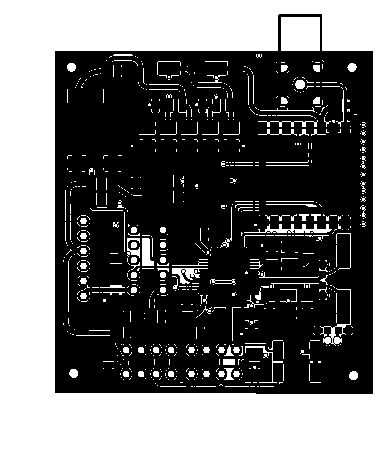
\includegraphics[width=0.7\linewidth]{Assets/PCB_Transmiter.pdf}
	\caption{تصویر برد مدار جاپی طراحی شده برای بخش سنسور.}
	\label{fig:PCBTransmiter}
\end{figure}

\begin{figure}[H]
	\begin{subfigure}[b]{0.5\textwidth}
		\includegraphics[width=\linewidth]{Assets/transmitterBack.png}
		\caption{پشت برد بخش سنسور}
		\label{fig:transmitterBack}
	\end{subfigure}
	\begin{subfigure}[b]{0.5\textwidth}
		\includegraphics[width=\linewidth]{Assets/transmitterFront.png}
		\caption{روی برد بخش سنسور}
		\label{fig:transmitterFront}
	\end{subfigure}
	\caption{تصاویر بردمدارچاپی طراحی‌شده برای بخش سنسور.}
	\label{fig:PCB3dviewtransmitte}
\end{figure}


\قسمت{نحوه ی طراحی بخش ایستگاه}
به طور کلی هدف از طراحی بخش ایستگاه، دریافت داده‌های ارسالی از ماژول لورا و مانیتور کردن آنها در PC می‌باشد. بلوک دیاگرام کلی بخش ایستگاه در شکل \رجوع{fig:Diagram2} نمایش داده شده است.

\begin{figure}[!h]
	\centering
	\includegraphics[width=0.7\linewidth]{Assets/diagram2.pdf}
	\caption{بلوک دیاگرام بخش ایستگاه.}
	\label{fig:Diagram2}
\end{figure}

\noindent
با توجه به بلوک دیاگرام شکل \رجوع{fig:Diagram2} داده‌‌های دریافتی از ماژول لورا توسط میکروکنترلر دریافت شده و توسط پروتکل \متن‌لاتین{USB} به رایانه فرستاده می‌شود و رایانه نیز توسط اپ طراحی شده دیتاهای دریافت شده را دریافت و مانتیور می‌‌کند.


\زیرقسمت{نقشه ی شماتیک بخش ایستگاه}

1- در این بخش که اصلی ترین قسمت مدار می‌باشد از خازن‌های 100 نانوفاراد و 1 میکروفاراد به منظور کاهش نویزهای فرکانس بالا و پایین استفاده شده است. همچنین در تغذیه ی ورودی میکروکنترلر علاوه بر این خازن‌ها از سلف به منظور کاهش ریپل جریان ورودی استفاده شده است. در این بخش از دو عدد کیرستال که یکی برای مدار اصلی و یکی برای قسمت \متن‌لاتین{RTC} استفاده شده است که خازن‌های آن مطابق با دیتاشیت میکروکنترلر انتخاب شده است. همانطور که در شکل مشاهده می‌شود قسمت دیتا و کلاک واحد \متن‌لاتین{I2C} با مقاومت‌های 4٫7 کیلو پول-آپ شده است.

\noindent
2-  این بخش مربوط به ماژول لورا می‌باشد. در این قسمت خازن برای کاهش نویز ورودی به ماژول استفاده شده است و همچنین یک کانکتور برای اتصال آنتن به ماژول قرار داده شده است. 

\noindent
3- در این بخش از یک رگولاتور ‌3٫3 ولت برای تغذیه‌ی ماژول آلتراسونیک استفاده شده است. ورودی رگولاتور،  تغذیه‌ای است که از بیرون به مدار اعمال می‌شود که حداقل می‌بایست 4٫3 ولت باشد و خروجی آن ولتاژ رگوله شده‌ی ‌3٫3 ولت می‌باشد. خازن‌های قرار داده شده در ورودی و خروجی رگولاتور به منظور کاهش ریپل ولتاژ ورودی به رگولاتور و کم کردن نویز خروجی رگولاتور استفاده شده است. همچنین در خروجی این رگولاتور یک دیود نورانی قرار داده شده است که با متصل کردن تغذیه‌ی ورودی روش می‌شود.

\noindent
4- در این بخش از یک کانکتور \متن‌لاتین{MICRO USB} برای برقراری ارتباط بین میکروکنترلر و رایانه استفاده شده است.

\noindent
5- این بخش که یک هدر 1x6 می‌باشد برای پروگرم و دیباگ کردن میکروکنترلر قرار داده شده است.

تصویر بردمدارچاپی طراحی‌شده برای سمت ایستگاه این پروژه در شکل \رجوع{fig:PCB3dviewreceiver} آمده است. همچنین تصاویر شماتیک آن در شکل \رجوع{fig:SchematicReciver} آمده است.
\begin{figure}[H]
	\includegraphics[width=\linewidth]{Assets/Schematic_Reciver.png}
	\caption{تصویر شماتیک برد مدارچاپی سمت ایستگاه.}
	\label{fig:SchematicReciver}
\end{figure}

\begin{figure}[H]
	\centering
	\includegraphics[width=0.7\linewidth]{Assets/PCB_Reciver.pdf}
	\caption{تصویر برد مدار چاپی طراحی شده برای بخش ایستگاه.}
	\label{fig:PCBReciver}
\end{figure}



\begin{figure}[H]
	\begin{subfigure}[b]{0.5\textwidth}
		\includegraphics[width=\linewidth]{Assets/receiverBack.png}
		\caption{پشت برد بخش ایستگاه}
		\label{fig:receiverBack}
	\end{subfigure}
	\begin{subfigure}[b]{0.5\textwidth}
		\includegraphics[width=\linewidth]{Assets/receiverFront.png}
		\caption{روی برد بخش ایستگاه}
		\label{fig:receiverFront}
	\end{subfigure}
	\caption{تصاویر بردمدارچاپی طراحی‌شده برای بخش ایستگاه.}
	\label{fig:PCB3dviewreceiver}
\end{figure}
	
	%!TeX root=../main.tex

\فصل{تشریح پروژه}
\قسمت{مقدمه}
\begin{figure}[!h]
	\centering
	\includegraphics[width=\linewidth]{Assets/system design.pdf}
	\caption{بلوک دیاگرام اجزای سیستم و نحوه ارتباط اجزای مختلف با یکدیگر.}
	\label{fig:systemDesign}
\end{figure}
این سیستم به دو دستگاه اصلی تقسیم می‌شود، یک دستگاه جهت جمع‌آوری اطلاعات جوی برروی یک میله در ارتفاع 10 متری سطح زمین قرار می‌گیرد و اطلاعات جوی نظیر دما، رطوبت، فشار، شدت نور، سرعت و جهت باد را از سنسورهای مربوطه جمع‌آوری کرده و به‌صورت بی‌سیم به دستگاه دیگر، که در ایستگاه اصلی قرار دارد، مخابره می‌کند؛ سپس اطلاعات دریافت شده در سمت دستگاه دوم جهت ثبت و ذخیره به رایانه منتقل می‌شود. در اینجا به دستگاه اول که وظیفه جمع‌آوری اطلاعات جوی را دارد سنسور و دستگاه دوم که وظیفه دریافت اطلاعات مخابره شده و انتقال به رایانه را دارد ایستگاه می‌گوییم. بلوک دیاگرام کلی این سیستم و نحوه ارتباط بخش‌های مختلف با یکدیگر در شکل \رجوع{fig:systemDesign} آمده است.

عملکرد کلی سیستم جمع‌آوری داده‌ها در سمت سنسور، ارسال اطلاعات از طریق لورا به سمت ایستگاه و نمایش اطلاعات دریافت شده در سمت ایستگاه برروی رایانه است. به‌طورکلی این سیستم به دو بخش سنسور و ایستگاه تقسیم می‌شود که بخش ایستگاه خود به دو بخش دستگاه گیرنده و برنامه دسکتاپ (\متن‌لاتین{Desktop}) قابل‌تقسیم است.

\قسمت{سنسور}
فلوچارت فرآیند‌های سمت سنسور در تصویر \رجوع{fig:SensorFlowChart} قابل مشاهده است شرح آن به قرار زیر است:
\شروع{فقرات}
\فقره
بعد از روشن شدن دستگاه و فعالسازی بخش‌های موردنیاز (\متن‌لاتین{peripherals})، میکروکنترلر از طریق \متن‌لاتین{I\بالانویس‌متنی{2}C} با سنسور \متن‌لاتین{BMP180} ارتباط برقرار می‌کند و ضرایب کالیبراسیو را از سنسور \متن‌لاتین{BMP180} می‌خواند این ضرایب برای محاسبه دما و فشار مورداستفاده قرار می‌گیرند \مرجع{sensortec2015digital}.
\فقره
میکروکنترلر با برقراری ارتباط از طریق \متن‌لاتین{I\بالانویس‌متنی{2}C} با سنسور \متن‌لاتین{MAX44009} مقدار رجیستر تنظیمات این سنسور را \متن‌لاتین{0x00} تنظیم می‌کند. در این حالت سنسور در پایین‌ترین سطح مصرف توان خوده قرار می‌گیرد و هر 800 میلی‌ثانیه یکبار میزان شدت نور را اندازه‌گیری می‌کند \مرجع{MAX44009}.
\فقره
با برقراری ارتباطی از طریق \متن‌لاتین{I\بالانویس‌متنی{2}C} با سنسور \متن‌لاتین{HMC5883L} و تنظیم رجیستر تنظیمات، سنسور در حالت آماده‌به‌کار و نرخ نمونه‌برداری 50 هرتز قرار می‌گیرد \مرجع{HMC5883L}.
\فقره
رجیسترهای تنظیمات ماژول \متن‌لاتین{LoRa} با برقراری ارتباط از طریق \متن‌لاتین{SPI} تنظیم‌شده و این ماژول در حالت آماده‌به‌کار قرار می‌گیرد. فرکانس این ماژول روی 433 مگاهرتز، توان آن روی 20 \متن‌لاتین{dBm}، ضریب بخش آن روی 10 و پهنای باند آن روی 31٫2 کیلوهرتز تنظیم می‌گردد (به‌منظور دریافت اطلاعات ارسالی در سمت ایستگاه نیز دقیقاً همین تنظیمات فرکانس، پهنای باند و ضریب پخش باید اعمال شوند) \مرجع{SX1278}.
\فقره
برنامه وارد حلقه اصلی کار خود شده و دما و فشار را با استفاده از سنسور \متن‌لاتین{BMP180} اندازه‌گیری می‌کند. 
\فقره
پس از اندازه‌گیری شدت نور با استفاده از سنسور \متن‌لاتین{MAX44009} \مرجع{MAX44009} و اندازه‌گیری رطوبت هوا به‌وسیله سنسور \متن‌لاتین{AHT10} \مرجع{AHT10}، جهت جغرافیایی توسط سنسور \متن‌لاتین{QMC5883L} \مرجع{HMC5883L} به‌دست می‌آید. 
\فقره
سرعت باد روی دو محور \متن‌لاتین{x} و \متن‌لاتین{y} با استفاده از سنسور \متن‌لاتین{HCSR05} و با توجه به رابطه‌ی \رجوع{eq:speedWindX} محاسبه می‌شود. سپس زاویه و شدت باد با توجه به‌سرعت باد روی هر دو محور با توجه به رابطه \رجوع{eq:windSpeed} به‌دست می‌آید.
\فقره
اطلاعات جمع‌آوری و محاسبه‌شده از طریق ماژول لورا برای گیرنده سمت ایستگاه ارسال می‌شود.
\فقره 
میکروکنترلر و سنسورها در حالت توقف\پانویس{Stop} قرار داده می‌شوند و پس از سه ساعت با رخ‌دادن آلارم\پانویس{Alarm} میکروکنترلر از حالت توقف خارج شده و فرآیند دریافت و ارسال داده‌ها را تکرار می‌کند.
\فقره 
پس از هر بار خارج شدن از حالت توقف، آلارم بعدی برای سه ساعت بعد تنظیم می‌شود.
\پایان{فقرات}

\begin{figure}[H]
	\centering
	\includegraphics[width=0.6\linewidth]{Assets/SensorFlowChart.pdf}
	\caption{فلوچارت برنامه سمت سنسور.}
	\label{fig:SensorFlowChart}
\end{figure}

\زیرقسمت{نحوه خواندن دما و فشار از سنسور \متن‌لاتین{BMP180}}
در ابتدا لازم است ضرایب کالیبراسیون از سنسور \متن‌لاتین{BMP180} دریافت شود. روش ارتباط این ماژول با میکروکنترلر از طریق پروتکل \متن‌لاتین{I2C} است. جهت خواندن مقادیر ضرایب کالیبراسیون باید آدرس \متن‌لاتین{MSB} رجیستر متناظر با هر ضریب را با مود \متن‌لاتین{Read} به آدرس ماژول (\متن‌لاتین{0x77}) ارسال نماییم و ماژول در پاسخ 16 بیت داده را به ما بر می‌گرداند که مقدار ضریب کالیبراسیون مورد نظر است. آدرس رجیستر‌های ضرایب کالیبراسیون در تصویر شکل \رجوع{fig:bmp180Calibrationcoefficient} آمده است.
\begin{figure}[H]
	\centering
	\includegraphics[width=0.5\linewidth]{Assets/bmp180Calibrationcoefficient.png}
	\caption{آدرس رجیستر ضرایب کالیبراسیون سنسور \متن‌لاتین{BMP180}.}
	\label{fig:bmp180Calibrationcoefficient}
\end{figure}

\زیرزیرقسمت{خواندن دما}
به جهت خواندن مقدار دما باید مقدار \متن‌لاتین{0x2E} را در رجیستر کنترل \متن‌لاتین{0xF4} بنویسیم. با این کار سنسور در حالت اندازه‌گیری دمای محیط قرار می‌گیرد و پس از حداکثر 4٫5 میلی ثانیه این داده برای خواندن آماده ‌می‌شود. این کار با ارسال مقدار آدرس رجیستر کنترل یعنی \متن‌لاتین{0xF4} در مود \متن‌لاتین{Write} به آدرس ماژول (\متن‌لاتین{0x77}) و پس از آن ارسال مقدار کنترل مورد نظر یعنی \متن‌لاتین{0x2E} انجام می‌شود. پس از اندازه‌گیری دما مقدار اندازه‌گیری شده در رجیستری با آدرس \متن‌لاتین{(MSB)0xF6} و \متن‌لاتین{(LSB)0xF7} در ماژول ذخیره می‌شود. به جهت خواندن مقدار اندازه‌گیری شده پس از حداقل 4٫۵ میلی ثانیه بعد از ارسال مقدار کنترلر \متن‌لاتین{0x2E} به ماژول باید مقدار \متن‌لاتین{MSB} رجیستر داده‌هایعنی \متن‌لاتین{0xF6} به آدرس سنسور (\متن‌لاتین{0x77}) در مود \متن‌لاتین{Read} فرستاده شود تا ماژول در پاسخ 16 بیت داده‌های اندازه گیری شده را که در این حالت مقدار دمای محیط است را به ما برگرداند (ابتدا مقدار رجیستر \متن‌لاتین{MSB} و سپس مقدار \متن‌لاتین{LSB} برگشت داده می‌شود). سپس مقدار دقیق دمای محیط با دقت 0.1 درجه سانتی گراد از طریق فرمول زیر قابل محاسبه خواهد بود:
\begin{fleqn}
	\begin{equation*}
		\begin{split}
			&UT = MSB << 8 + LSB \\
			&X1 = (UT - AC6) * AC5 / 2^{15} \\
			&X2 = MC * 2^{11} / (X1 + MD) \\
			&B5 = X1 + X2 \\
			&T = (B5 + 8) / 2^4
		\end{split}
	\end{equation*}
\end{fleqn}
\noindent
که $AC6$، $AC5$، $MD$ و $MC$ ضرایب کالیبراسیون، $MSB$ مقدار \متن‌لاتین{MSB} رجیستر داده‌های دریافت شده، $LSB$ مقدار \متن‌لاتین{LSB} رجیستر داده‌های دریافت شده و $T$ دمای محیط بر حسب سانتی‌گراد خواد بود.

\زیرزیرقسمت{خواندن فشار}
طریقه خواندن فشار از ماژول نیز مشابه خواندن دما است. در ابتدا لازم باید مقدار رجیستر کنترل ماژول را با مقدار مورد نظر (که در اینجا مقدار متناظر با دریافت فشار است) پر کرد و پس از زمانی مشخص داده‌های اندازه گیری شده را از رجیستر‌های داده ماژول خواند. در حالت خواندن فشار بر خلاف خواندن دما ماژول حالت‌های نمونه‌بردادی مختلفی را ارائه می‌کند که باید بر اساس نیاز مقدار مربوط به هر مود نمونه برداری که مد نظر بود را در رجیستری کنترل نوشت تا ماژول در حالت نمونه برداری مورد نظر قرار گیرد. با افزایش نرخ نمونه برداری دقت مقدار اندازه‌گیری شده بیشتر شده ولی زمانی که ماژول صرف اندازه‌گیری می‌کند نیز افزایش می‌یابد. در جدول \رجوع{table:BMP180persure} مقدار رجیستر کنترلی متناظر با هر مود نمونه برداری و حداکثر زمان لازم برای انجام نمونه برداری آورده شده است. 

\begin{table}[!h]
	\centering
	\caption{حالت‌های نمون برداری فشار ماژول \متن‌لاتین{BMP180}.}
	\label{table:BMP180persure}
	\begin{tabular}{ccc}
		حالت نمونه برداری & مقدار رجیستر کنترلی & حداکثر زمان اندازه‌گیری (میلی‌ثانیه)\\
		\hline
		0 & \متن‌لاتین{0x34} & 4٫5 \\
		1 & \متن‌لاتین{0x74} & 7٫5 \\
		2 & \متن‌لاتین{0xB4} & 13٫5 \\
		3 & \متن‌لاتین{0xF4} & 25٫5 \\
		
	\end{tabular}
\end{table}

در این پروژه استفاده از مود نمونه برداری 0 برای ما کفایت می‌کند. برای محاسبه فشار اندازه گیری دمای هوا نیز لازم است پس ابتدا لازم است قبل از درخواست اندازه گیری فشار دمای محیط توسط روشی که قبل تر گفته شد اندازه گیری شود. به جهت خواندن مقدار فشار باید مقدار \متن‌لاتین{0x34} را در رجیستر کنترل \متن‌لاتین{0xF4} بنویسیم (مود 0). با این کار سنسور در حالت اندازه‌گیری فشار قرار می‌گیرد و پس از حداکثر 4٫5 میلی ثانیه (با توجه به جدول \رجوع{table:BMP180persure} و در مود 0) این داده برای خواندن آماده ‌می‌شود. این کار با ارسال مقدار آدرس رجیستر کنترل یعنی \متن‌لاتین{0xF4} در مود \متن‌لاتین{Write} به آدرس ماژول (\متن‌لاتین{0x77}) و پس از آن ارسال مقدار کنترل مورد نظر یعنی \متن‌لاتین{0x34} انجام می‌شود. پس از اندازه‌گیری فشار مقدار اندازه‌گیری شده در رجیستری با آدرس \متن‌لاتین{(MSB)0xF6}،\متن‌لاتین{(LSB)0xF7} و \متن‌لاتین{0xF8(XLSB)} در ماژول ذخیره می‌شود. به جهت خواندن مقدار اندازه‌گیری شده پس از حداقل 4٫۵ میلی ثانیه بعد از ارسال مقدار کنترل \متن‌لاتین{0x34} (در مود 0) به ماژول باید مقدار \متن‌لاتین{MSB} رجیستر داده‌هایعنی \متن‌لاتین{0xF6} به آدرس سنسور (\متن‌لاتین{0x77}) در مود \متن‌لاتین{Read} فرستاده شود تا ماژول در پاسخ 16 بیت داده‌های اندازه گیری شده را به ما برگرداند (ابتدا مقدار رجیستر \متن‌لاتین{MSB} و سپس مقدار \متن‌لاتین{LSB} برگشت داده می‌شود) و سپس باید مقدار \متن‌لاتین{XLSB} رجیستر داده‌هایعنی \متن‌لاتین{0xF8} به آدرس سنسور (\متن‌لاتین{0x77}) در مود \متن‌لاتین{Read} فرستاده شود تا ماژول در پاسخ 8 بیت داده‌ را به ما برگرداند. سپس مقدار دقیق فشار محیط با دقت 1 پاسکال از طریق فرمول زیر قابل محاسبه خواهد بود:

\begin{fleqn}
	\begin{equation*}
	\begin{split}
		&UP = (MSB<<16 + LSB<<8 + XLSB) >> (8-oss) \\
		&B6 = B5 - 4000 \\
		&X1 = (B2 * (B6 * B6 / 2^{12} )) / 2^{11}\\
		&X2 = AC2 * B6 / 2^{11}\\
		&X3 = X1 + X2\\
		&B3 = ((AC1*4+X3) << oss + 2) / 4\\
		&X1 = AC3 * B6 / 2^{13}\\
		&X2 = (B1 * (B6 * B6 / 2^{12} )) / 2^{16}\\
		&X3 = ((X1 + X2) + 2) / 2^2\\
		&B4 = AC4 * (unsigend long)(X3 + 32768) / 2^{15}\\
		&B7 = ((unsigned long)UP - B3) * (50000 >> oss)\\
		&if (B7 < 0x80000000) \{ p = (B7 * 2) / B4 \}\\
	\end{split}
	\end{equation*}
\end{fleqn}

\begin{fleqn}
	\begin{equation*}
	\begin{split}
		&else \{ p = (B7 / B4) * 2 \}\\
		&X1 = (p / 2^8 ) * (p / 2^8 )\\
		&X1 = (X1 * 3038) / 2^{16}\\
		&X2 = (-7357 * p) / 2^{16}\\
		&p = p + (X1 + X2 + 3791) / 2^{16}
		\end{split}
	\end{equation*}
\end{fleqn}
\noindent
که $B5$ مقدار بدست آمده از روابط محاسبه دما است که در بخش قبلی بیان شده است، $oss$ عدد مود نرخ نمونه برداری (از 0 تا 3 مطابق جدول \رجوع{table:BMP180persure})، $AC1$، $AC2$، $AC3$، $AC4$، $B1$ و $B2$ ضرابیب کالیبراسیون، $MSB$ مقدار \متن‌لاتین{MSB} رجیستر داده‌های دریافت شده، $LSB$ مقدار \متن‌لاتین{LSB} رجیستر داده‌های دریافت شده ، $XLSB$ مقدار رجیستر داده \متن‌لاتین{XLSB} و در نهایت p مقدار فشار اندازه‌گیری شده بر حسب پاسکال خواهد بود. 

\زیرقسمت{نحوه خواندن شدت نور از سنسور \متن‌لاتین{MAX44009}}
در ابتدا پس از روشن شدن ماژول لازم است که حالت کاری ماژول و تنظیمات اولیه آن انجام شود. این کار با نوشتن رجیستر کنترلی این ماژول با آدرس \متن‌لاتین{0x02} انجام می‌شود. بیت هشتم این رجیستر به بین \متن‌لاتین{CONT} معروف است. این بیت مسئول تعیین مود کارکرد است به طوری که اگر مقدار $0$‍ در آن نوشته شود ماژول هر 800 میلی‌ثانیه مقدار نور محیط را اندازه‌گیری کرده و در رجیتسر‌های خود ذخیره می‌کند و اگر مقدار $1$ در آن نوشته شده باشد ماژول بدون وقفه و پشت‌سر‌هم اندازه‌گیری نور را انجام می‌دهد. برای این پروژه استفاده از مود $0$ مناسب تر است و ازین مود استفاده خواهیم کرد. بیت هفتم این رجیستر به بیت \متن‌لاتین{MANUAL} معروف است و در صورتی که با $1$ پر شود کاربر قادر به مشخص کردن مقادیر \متن‌لاتین{CDR} و \متن‌لاتین{TIM[2:0]} خواهد بود و در غیر این صورت خوده سیستم در مورد این مقادیر تصمیم گیری می‌کند. مقدار \متن‌لاتین{CDR} که بیت چهارم رجیستر کنترل است، مشخص کننده مقدار مقسم مقادیر خوانده شده از \متن‌لاتین{ADC} است و در صورتی که با $0$ پر شده باشد هیچ عملیات تقسیمی رخ نداده و مقادیر \متن‌لاتین{ADC} عینا در رجیستر‌ها کپی می‌شوند و در صورتی که با مقدار $1$ پر شده باشد مقادیر تقسیم بر 8 می‌شوند (در مواقعی که نور محیط بسیار زیاد است کاربرد دارد). مقدار \متن‌لاتین{TIM[2:0]} نیز که بیت اول تا سوم رجیستر کنترل را به خود اختصاص داده بیان کننده زمان نمونه برداری و اذغام است که مقادیر متناظر با حالت‌های مختلف قابل انتخاب برای این بیت‌ها در جدول \رجوع{table:BMP180persure} آمده است. در حالت خودکار زمان‌هایی بین 100 تا 800 میلی ثانیه انتخاب می‌شوند و در حالت دستی میتوان از 6.25 میلی ثانیه تا 800 میلی ثانیه را انتخاب کرد. حالت 800 میلی ثانیه مناسب محیط با نور بسیارکم و حالت 6.25 میلی ثانیه مناسب محیط‌هایی با نور بسیار زیاد است. 

\begin{table}[!h]
	\centering
	\caption{مقادیر بیت‌های \متن‌لاتین{TIM[2:0]}.}
	\label{table:BMP180persure}
	\begin{tabular}{c|c}
		\متن‌لاتین{TIM[2:0]} & زمان نمونه برداری و ادغام (میلی‌ثانیه)\\
		\hline
		$000$ & 800 \\
		$001$ & 400 \\
		$010$ & 200 \\
		$011$ & 100 \\
		$100$ & 50 \\
		$101$ & 25 \\
		$110$ & 12٫5 \\
		$111$ & 6٫25 \\
	\end{tabular}
\end{table}
\noindent
در این پروژه به دلیل ثابت نبودن شرایط محیطی انتخاب حالت خودکار (مقدار $0$ برای \متن‌لاتین{MANUAL}) مناسب ترین روش ممکن است. با این کار مقادیر \متن‌لاتین{CDR} و \متن‌لاتین{TIM[2:0]} توسط خوده ماژول و با توجه به شرایط محیطی در هر اندازه گیری مشخص می‌شود. پس در این پروژه لازم است پس از روشن شدن ماژول مقدار \متن‌لاتین{0x00} در رجیستر کنترل به آدرس \متن‌لاتین{0x02} نوشته شود. این کار با ارسال آدرس رجیستر (\متن‌لاتین{0x02}) در مود \متن‌لاتین{Write} به آدرس ماژول (\متن‌لاتین{0x4A}) و پس از آن ارسال مقدار \متن‌لاتین{0x00} انجام می‌شود. با این کار ماژول ماکسیموم هر 800 میلی ثانیه یک بار دیتا‌های جدید را اندازه‌گیری کرده و در رجیستر‌هایی با آدرس \متن‌لاتین{0x03(MSB)} و \متن‌لاتین{0x04(LSB)} ذخیره می‌کند به جهت خواندن این مقادیر لازم است آدرس رجیستر به آدرس ماژول در مود \متن‌لاتین{Read} فرستاده شود تا ماژول در پاسخ 8 بیت دیتای این رجیستر‌ها را به ما برگرداند. پس از دریافت این مقادیر شدت نور بر حسب لوکس از طریق روابط زیر قابل محاسبه خواهد بود:
\begin{fleqn}
	\begin{equation*}
		Lux = (2^{Exponent} \times Mantissa) \times 0.045
	\end{equation*}
\end{fleqn}
\noindent
که مقادیر $Exponent$ و $Mantissa$ از روی مقادیر رجیستر‌های \متن‌لاتین{0x03(MSB)} و \متن‌لاتین{0x04(LSB)} و از طریق روابط زیر و جدول \رجوع{table:MAX44009DataRegisters} بدست می‌آیند.

\begin{table}[!h]
	\centering
	\caption{مقدار رجیستر‌های \متن‌لاتین{0x03(MSB)} و \متن‌لاتین{0x04(LSB)}.}
	\label{table:MAX44009DataRegisters}
	\begin{tabular}{c|cccccccc}
		رجیستر & $bit 0$ & $bit 1$ & $bit 2$ & $bit 3$ & $bit 4$ & $bit 5$ & $bit 6$ & $bit 7$\\
		\hline
		\متن‌لاتین{0x03} & $M4$ & $M5$ & $M6$ & $M7$ & $E0$ & $E1$ & $E2$ & $E3$ \\
		\متن‌لاتین{0x04} & $M0$ & $M1$ & $M2$ & $M3$ & - & - & - & - \\
	\end{tabular}
\end{table}


\begin{fleqn}
	\begin{equation*}
		Exponent = 8\times E3 + 4\times E2 + 2\times E1 + E0\\
	\end{equation*}
\end{fleqn}
\begin{fleqn}
	\begin{equation*}
	\begin{split}
		Mantissa = &128\times M7 + 64\times M6 + 32\times M5 + 16\times M4 \\
					&+ 8\times M3 + 4\times M2 + 2\times M1 + M0
	\end{split}
	\end{equation*}
\end{fleqn}


\زیرقسمت{نحوه دریافت جهت جغرافیایی از سنسور \متن‌لاتین{QMC5883L}}
در ابتدا پس از روشن شدن ماژول لازم است رجیستر‌ کانفیک این ماژول تنظیم شده و ماژول در مود کاری مورد نظر قرار بگیرد. بیت‌ها و تنظیمات متناظر با اطلاعات پر شده در این رجیستر در جدول تصویر \رجوع{fig:QMC5883LControlRegister} قابل مشاهده است. 

\begin{figure}[H]
	\centering
	\includegraphics[width=0.9\linewidth]{Assets/QMC5883LControlRegister.png}
	\caption{رجیستر کانفیگ ماژول \متن‌لاتین{QMC5883L}.}
	\label{fig:QMC5883LControlRegister}
\end{figure}
\noindent
برای شروع به کار و نمونه برداری، مود کاری باید در حالت \متن‌لاتین{continuous} قرار بگیرد.  برای این پروژه ریت خروجی 10 یا 50 هرتز و ریت نمونه برداری 2 گاوس مناسب اند. مقدار \متن‌لاتین{OSR} را نیز بیشترین حالت یعنی 512 در نظر می‌گیریم. پس مقدار رجسیتر کانفیگ باید با \متن‌لاتین{0x05} پر شود. برای این کار باید مقدار آدرس رجیستر کانفیگ (\متن‌لاتین{0x09}) را به در مود \متن‌لاتین{Write} به آدرس ماژول (\متن‌لاتین{0x0D}) ارسال کنیم و پس از آن مقدار مورد نظر را (\متن‌لاتین{0x05}) ارسال نماییم. با این کار ماژول وارد مود کار بدون وقفه خود شده و پس از اندازه گیری‌ و ذخیره اطلاعات در رجیستر‌های خود اولین بیت رجیستر حالت خود به آدرس \متن‌لاتین{0x06} را به نشانه وجود داده برای دریافت 1 می‌کند. پس با خواندن رجیستر حالت این ماژول میتوانیم از وجود یا عدم وجود داده برای دریافت باخبر شویم. این کار را با ارسال آدرس رجیستر حالت (\متن‌لاتین{0x06}) در مود \متن‌لاتین{Read} به آدرس ماژول (\متن‌لاتین{0x0D}) انجام می‌دهیم و ماژول در پاسخ 8 بیت داده‌های رجیستر حالت را به ما برمی‌گرداند. در صورت 1 بودن اولین بیت رجیستر حالت داده‌ها برای دریافت آماده‌اند و لازم است آن‌ها را از رجیستر‌های داده بخوانیم. رجیستر‌های \متن‌لاتین{0x00(LSB)} و \متن‌لاتین{0x01(MSB)} حاوی اطلاعات محور \متن‌لاتین{X}، رجیستر‌های \متن‌لاتین{0x02(LSB)} و \متن‌لاتین{0x03(MSB)} حاوی اطلاعات محور \متن‌لاتین{Y} و رجیستر‌های \متن‌لاتین{0x05(LSB)} و \متن‌لاتین{0x06(MSB)} حاوی اطلاعات محور \متن‌لاتین{Z} هستند. با دریافت این اطلاعات به راحتی با انجام محاسبات ریاضی میتوان زاویا با محور‌های مختصات را بدست آورد. در این پروژه زاویه بردار روی صفحه \متن‌لاتین{X} و متن‌لاتین{Y} با بردار \متن‌لاتین{X} برای ما اهمیت دارد که با توجه به فرمول زیر بدست می‌آید:

\begin{fleqn}
	\begin{equation*}
		angle = \arctan{\frac{Y}{X}}
	\end{equation*}
\end{fleqn}

\زیرقسمت{نحوه خواندن رطوبت از سنسور \متن‌لاتین{AHT10}}
این سنسور بر خلاف سنسور‌های دیگه نیازی به کانفیگ برای اندازه‌گیری و کالیبراسیون ندارد و پس از روشن شدن میتوان آن را در حالت دریافت اطلاعات قرار داد و پس از حداقل 75 میلی‌ثانیه داده‌ها را از این سنسور خواند. این سنسور علاوه بر رطوبت دمای هوا را نیز اندازه گیری می‌کند ولی دقت آن در اندازه‌گیری دمای هوا به اندازه ماژول \متن‌لاتین{BMP180} نیست و از این رو داده‌های دمای هوایی که این سنسور اندازه‌گیری می‌کند را در این پروژه نادیده می‌گیریم.

برای قرار گرفتن ماژول در مود اندازه‌گیری باید دیتا‌های \متن‌لاتین{0xAC}، \متن‌لاتین{0x33} و \متن‌لاتین{0x00} را به همین ترتیب به آدرس ماژول (\متن‌لاتین{0x38}) ارسال کرد. با این کار ماژول ر حالت اندازه‌گیری قرار میگیرد و حداقل 75 میلی‌ثانیه بعد دیتا‌های اندازه‌گیری شده را در قالب 48 بیت به ما برمی‌گرداند این دیتا‌ها را هر هشت بیت با نام \متن‌لاتین{Data0} تا \متن‌لاتین{Data5} نام گذاری می‌کنیم. فشار نسبی هوا برحسب درصد از طریق روابط زیر و با استفاده از مقادیر برگشت داده شده از ماژول قابل محاسبه خواهد بود:

\begin{fleqn}
	\begin{equation*}
	\begin{split}
		&S_{RH} = Data1 \times 2^{12} +  Data2 \times 2^4 + Data3 / 2^4\\
		&RH = (S_{RH} * 100 / 2^{20});
	\end{split}
	\end{equation*}
\end{fleqn}

که $Data1$ تا $Data3$ مقادیر برگشت داده شده از سنسور و $RH$ مقدار رطوبت نسبی برحسب درصد است. 

\زیرقسمت{نحوه محاسبه سرعت و جهت باد}
جهت محاسبه سرعت و جهت باد ابتدا باید سرعت باد روی دو محور \متن‌لاتین{X} و \متن‌لاتین{Y} را بدست آورد. برای این کار در ابتدا نیاز به محاسبه سرعت صوت خواهد بود. سرعت صوت با توجه به روابطی که در بخش \رجوع{sec:windSpeedANDAngle} بیان شده است به عنوان تابعی از دمای هوا، رطوبت و فشار قابل محاسبه است. با وجود فاصله‌ای ثابت و مشخص بین فرستنده و گیرنده‌های آلتراسونیک،بنا به روابط بیان شده در بخش \رجوع{sec:windSpeedANDAngle}، زمانی که طول می‌کشد موج آلتراسونیک از فرستنده به گیرنده برسد با سرعت صورت به اضافه سرعت باد متناسب خواهد بود. پس با داشتن سرعت صوت و فاصله بین گیرنده و فرستنده و محاسبه زمانی که طول می‌کشد موج آلتراسونیک از فرستنده به گیرنده برسد می‌توان سرعت باد را محاسبه کرد.

برای محاسبه زمانی که طول می‌کشد تا موج آلتراسونیک از فرستنده به گیرنده برسد از ماژول \متن‌لاتین{HCSR05} بهره گرفتیم. این ماژول با دریافت پالسی با طول حداقل 10 میکرو ثانیه، موج آلتراسونیکی با فرکانس 40 کیلوهرتز تولید می‌کند. این ماژول هنگامی که پالس آلتراسونیک را تولید و ارسال می‌کند خروجی خود را 1 می‌کند و آن را تا زمانی که پالس آلتراسونیک را از گیرنده خود دریافت کند 1 نگه‌می‌دارد. در حقیقت با اندازه‌گیری طول پالس تولید شده در خروجی این ماژول زمانی که طول می‌کشد پالس آلتراسونیک از گیرنده به فرستنده برسد بدست می‌آید (این زمان به زمان پرواز معروف  است). این زمان را با استفاده از واحد تایمر در میکروکنترلر اندازه‌گیری میکنیم به طوری که زمانی که پالسی با لبه بالا رونده روی پایه خروجی ماژول رخ داد شمارش تایمر را شروع کرده و هر یک میکرو ثانیه (دقت خروجی ماژول در این حد است) شمارش می‌کند و سپس زمانی که پالسی با لبه پایین رونده رخ داد شمارش را متوقف می‌کند و عدد شمارنده در این حالت همان زمان به اصطلاح پرواز ما خواهد بود.

با محاسبه زمان پرواز و با توجه به روابط ارائه شده در بخش \رجوع{sec:windSpeedANDAngle} میتوان سرعت باد را بدست آورد. برای محاسبه جهت باد لازم است سرعت باد روی هر دو محور مختصاتی \متن‌لاتین{X} و \متن‌لاتین{Y} بدست بیاید. با داشتن سرعت باد روی هر دو محور میتوان این مقادیر را به دستگاه مختصات قطبی برد تا اندازه و زاویه وزش باد نسبت به محور \متن‌لاتین{X} مختصات را در دست داشت. در این حالت اندازه در مختصات قطبی همان سرعت باد مد نظر ما است و با جمع کردن زاویه بدست آمده در این حالت با زاویه بدست آمده از سنسور قطب نما ($angle$) جهت باد بدست می‌آید. البته لازم است در این حالت محور‌های مختصات سنسور باد منطبق با محور‌های مختصات سنسور قطب‌نما باشند در غیر این صورت باید اختلاف زاویه این دو محور مختصات را نیز در محاسبات لحاظ کرد.

\زیرقسمت{نحوه ارسال اطلاعات از طریق لورا}\label{sec:loraConfig}
در ابتدا پس از روشن کردن لورا باید مقادیر رجیستر‌های کانفیگ آن را با مقادیر مورد نیاز پر کرد و آن را در مود کاری مورد نیاز قرار داد. به جهت نوشتن رجیستر‌های کانفیگ لورا باید در ابتدا این ماژول را در مود اسلیپ قرار داد. تنها در این حالت مقادیر نوشته شده به عنوان کانفیگ روی ماژول اعمال می‌شوند. برای این کار باید مقدار رجیستر \متن‌لاتین{RegOpMode} با آدرس \متن‌لاتین{0x01} با مقدار \متن‌لاتین{0x08} پر شود. برای این کار پس از انتخاب چیپ با پایه \متن‌لاتین{NSS}، مقدار \متن‌لاتین{0x01} و سپس \متن‌لاتین{0x08} روی پایه \متن‌لاتین{MOSI} ارسال می‌شود. با این کار ماٰژول لورا در حالت اسپیلپ و آماده اعمال تنظیمات قرار می‌گیرد. حال مقدار رجیستر‌های \متن‌لاتین{RegFrMsb}، \متن‌لاتین{RegFrMid} و \متن‌لاتین{RegFrLsb} به آدرس‌های \متن‌لاتین{0x06}، \متن‌لاتین{0x07} و \متن‌لاتین{0x08} را که تنظیم کننده فرکانس موج رادیویی اند را با مقادیر \متن‌لاتین{0x6C}، \متن‌لاتین{0x40} و \متن‌لاتین{0x00} پر میکنیم (این مقدار از تقسیم فرکانس مورد نظر بر  61٫03515625 بدست آمده است). با این کار فرکانس کاری روی 433 مگاهرتز تنظیم می‌شود. حال باید رجیستر \متن‌لاتین{RegPaConfig} به آدرس \متن‌لاتین{0x09} را مقدار دهی کنیم. این رجیستر تنظیم کننده توان خروجی است. برای توان خروجی 20 \متن‌لاتین{dB} باید مقدار \متن‌لاتین{0x8F} را در این رجیستر قرار دهیم. برای قرار دادن پهنای باند ماژول در حالت 250 کیلو هرتز لازم است 4 بیت آخر رجیستر \متن‌لاتین{RegModemConfig1} به آدرس \متن‌لاتین{0x1D} با مقدار \متن‌لاتین{0b1000} پر شود. همچنین برای تعیین ضریب پخش 10 لازم است 4 بیت آخر رجیستر رجیستر \متن‌لاتین{RegModemConfig2} به آدرس \متن‌لاتین{0x1E} با مقدار \متن‌لاتین{0b1010} پر شود. به جهت دریافت وضعیت ارسال پیام از طریق پایه‌های \متن‌لاتین{DIO} لازم است بیت اول رجیستر \متن‌لاتین{RegDioMapping2} با مقدار \متن‌لاتین{1} پر شود. در این حالت در صورت ارسال داده‌ها پایه \متن‌لاتین{DIO0} فعال می‌شود و ما با چک کردن وضعیت این پایه بعد از اعمال دستور ارسال می‌توانیم از وضعیت ارسال بسته باخبر شویم. 

\begin{figure}[H]
	\centering
	\includegraphics[width=0.6\linewidth]{Assets/sensorData.pdf}
	\caption{ساختار داده‌های موجود در سمت سنسور.}
	\label{fig:sensorData}
\end{figure}

پس از تنظیم رجیستر‌های کانفیگ ماژول را به حالت اسندبای میبریم در این حالت دیگر رجیستر‌های کانفیگ قابل تغییر نخواهند بود. برای این کار مقدار \متن‌لاتین{0x09} را درون رجیستر \متن‌لاتین{RegOpMode} می‌نویسیم. جهت ارسال داده باید رجیستر \متن‌لاتین{RegFifo} را با داده‌ مورد نظر پر کرد و سپس مود کاری را در حالت \متن‌لاتین{Tx} قرار‌ داد. برای قرار دادن ماژول در مود \متن‌لاتین{Tx} تنها کافیست مقدار \متن‌لاتین{0x8B} را درون رجیستر \متن‌لاتین{RegOpMode} (با آدرس \متن‌لاتین{0x01}) نوشت. داده‌های دریافت شده در سمت سنسور در آرایه‌ای از نوع \متن‌لاتین{float} ذخیره شده اند. ساختار این داده‌ها را در تصویر \متن‌لاتین{fig:sensorData} مشاهده می‌کنید. برای جای دادن داده‌ها در رجیستر \متن‌لاتین{FIFO} ماژول لورا لازم است داده‌ها در ساختاری 8 بیتی (آرایه‌ای از اعداد بدون علامت 8 بیتی) برای ماژول ارسال شوند از این رو مقادیر موجود در آرایه داده‌ها هر 8 بیت به هشت بیت به ماژول لورا و رجیستر \متن‌لاتین{FIFO} این ماژول فرستاده می‌شوند. ساختار داده‌های ارسالی به رجیستر \متن‌لاتین{FIFO} لورا نیز در تصویر \رجوع{fig:loraData} قابل مشاهده است. این داده‌ها با همین ساختار به طرف ایستگاه فرستاده و دریافت می‌شوند و لازم است پس از دریافت دوباره به ساختار اصلی و قبلی خود تبدیل شوند. 

\begin{figure}[H]
	\centering
	\includegraphics[width=0.4\linewidth]{Assets/loraData.pdf}
	\caption{ساختار داده‌های ارسالی از طریق لورا.}
	\label{fig:loraData}
\end{figure}

\زیرقسمت{پیکربندی \متن‌لاتین{I2C}}
برای نوشتن کد‌های این پروژه از لایبری \متن‌لاتین{HAL} استفاده می‌کنیم. در این صورت برای فعال کردن بخش \متن‌لاتین{I2C} تنها لازم است این بخش را در نرم افزار \متن‌لاتین{STM32CubeMX} فعال کنیم. تنظیمات این بخش مثل سرعت و نوع آدرس وابسته به دستگاه‌های \متن‌لاتین{Slave} متصل به \متن‌لاتین{I2C} است و باید با توجه به مواردی که آن‌ها پشتیبانی می‌کنند تنظیمات این قسمت را پر کرد. خوشبختانه تمامی سنسور‌های استفاده شده برای این پروژه تنظیمات یکسانی را پشتیبانی می‌کنند و می‌توان تنها با یک \متن‌لاتین{I2C} با تمامی آن‌ها ارتباط برقرار و دیتا‌های لازم را دریافت کرد. سنسور‌های استفاده شده همگی از ماکسیموم سرعت قابل استفاده یعنی 400 کیلوهرتز پشتیبانی می‌کنند اما در مورد این پروژه سرعت تبادل داده‌ها با سنسور‌ها تفاوت زیادی نمی‌کند. پس در نتیجه سرعت 100 کیلوهرتز را برای تست وتوسعه به امید کمتر کردن خطا‌های ممکن انتخاب می‌کنیم. تصویر تنظیمات این بخش در نرم افزار \متن‌لاتین{STM32CubeMX} در شکل \رجوع{fig:i2cConfig} آمده است. 

\begin{figure}[H]
	\centering
	\includegraphics[width=0.6\linewidth]{Assets/i2cConfig.png}
	\caption{تنظیمات \متن‌لاتین{I2C}.}
	\label{fig:i2cConfig}
\end{figure}

\زیرقسمت{پیکربندی \متن‌لاتین{SPI}}
به سبب اسفاده از لایبری \متن‌لاتین{HAL} و نرم افزار \متن‌لاتین{STM32CubeMX} برای فعال کردن این بخش از میکروکنترلر تنها کافی است این بخش را در نرم اقزار \متن‌لاتین{STM32CubeMX} فعال کنیم. برای این کار \متن‌لاتین{SPI} مورد نظر را در حالت \متن‌لاتین{Full-Duplex Master} قرار می‌دهیم. تنظیم پارامتر‌های دیگر بستگی به تنظیمات قابل پشتیبانی برای \متن‌لاتین{Slave}‌ها دارد. در این حالت برای ماژول لورا تنظیمات تصویر \رجوع{fig:SPIConfig} را اعمال می‌کنیم. ماژول لورا سرعت‌های تبادل بالاتر را نیز ساپورت می‌کند ولی در این پروژه سرعت تبادلات تفاوت زیادی ایجاد نمی‌کند از این رو برای تست وتوسعه به استفاده از سرعت‌های تبادل پایین تر بسنده می‌کتیم. 

\begin{figure}[H]
	\centering
	\includegraphics[width=0.6\linewidth]{Assets/SPIConfig.png}
	\caption{تنظیمات \متن‌لاتین{SPI}.}
	\label{fig:SPIConfig}
\end{figure}
\زیرقسمت{حالت توقف میکروکنترلر}
در این پروژه لازم است اطلاعات سنسور‌ها هر 3 ساعت یکبار جمع آوری و از طریق ماژول لورا مخابره شود و در بین این ساعات میکرو عملکرد دیگری نخواد داشت. برای ذخیره انرژی میتوان میکرو را در بین این ساعات در حالت توقف یا \متن‌لاتین{Stop} قرار داد. در حالت توقف مصرف انرژی میکرو کنترلر با غیر فعال کردن کلاک‌ها بسیار کاهش می‌یابد. در این مود مقادیر رم و رجیستر‌ها حفظ می‌شود و فقط کلاک‌ها غیر فعال می‌شوند. بعد از برخواستن از این حالت سیستم از کلاک \متن‌لاتین{HSI} به عنوان منبع کلاک استفاده می‌کند که لازم است در این حالت برای برگشت به حالت کار عادی تنظیمات کلاک دوباره اعمال شوند. در این حالت میکروکنترلر تنها مصرفی در حدود 0٫8 میکروآمپر را دارا می‌باشد (با فعال بودن \متن‌لاتین{RTC}). 

تفاوت این حالت با حالت \متن‌لاتین{Standby} که در آن میکرو کمترین میزان مصرف انرژی خود را دارد در این است که در حالت \متن‌لاتین{Standby} مقادیر رجیستر‌ها و رم ذخیره نمی‌شود (فقط رجیستر‌های مربوط به حالت \متن‌لاتین{Standby} دست نخورده باقی می‌مانند و باقی اطلاعات از دست می‌روند) و میکرو پس از برخواستن از این حالت وضعیتی مشابه وضعیت ریست شدن را خواهد داشت اما می‌توان مصرف را در حالتی مشابه تا 0٫57 میکرو‌آمپر کاهش داد.

برای خارج کردن میکروکنترلر از این حالت می‌توان از اینتراپت خارجی و یا آلارم واحد \متن‌لاتین{RTC} استفاده کرد. در این پروژه ما از آلارم واحد \متن‌لاتین{RTC} استفاده می‌کنیم. اولین آلارم را میتوان با استفاده از نرم افزار \متن‌لاتین{STM32CubeMX} در بخش \متن‌لاتین{RTC} تنظیم کرد و پس از آن با رخ دادن هر آلارم باید آلارم بعدی را برای سه ساعت بعد تنظیم کرد. 


\قسمت{ایستگاه}
فلوچارت فرآیند‌های سمت ایستگاه در تصویر \رجوع{fig:StationFlowChart} قابل مشاهده است شرح آن به قرار زیر است:
\شروع{فقرات}
\فقره 
با اتصال دستگاه از طریق کابل \متن‌لاتین{USB} به رایانه میکروکنترلر پس از فعال‌سازی بخش‌های موردنیاز، از طریق \متن‌لاتین{SPI} با ماژول لورا ارتباط برقرار کرده و رجیسترهای تنظیمات را با اطلاعات مشابه با سمت سنسور پر می‌کند و ماٰژول لورا را در حالت دریافت اطلاعات بدون توقف \پانویس{Continuously} قرارمی‌هد \مرجع{SX1278}.
\فقره 
میکرو به حلقه اصلی کار خود واردشده و پس از چک کردن وجود دیتای دریافتی در ماژول لورا، در صورت عدم وجود دیتا به حالت خواب \پانویس{Sleep} رفته و تا زمان دریافت دیتا در همان حالت باقی می‌ماند.
\فقره 
با دریافت دیتا توسط ماژول لورا وقفه‌ای خارجی رخ‌داده و میکرو را از حالت خواب بیدار می‌کند.
\فقره
میکرو کنترلر با برقراری ارتباط از طریق \متن‌لاتین{SPI} با ماژول لورا دیتای دریافت شده را خوانده و پس از بررسی یکسان بودن شناسه دریافت‌کننده با شناسه خود آن را از طریق \متن‌لاتین{USB} به رایانه ارسال می‌کند.
\فقره 
در صورت عدم وجود دیتاهای دیگر، میکرو کنترلر به حالت خواب رفته و تا رخ دادن وقفه بعدی، که نشان‌دهنده دریافت اطلاعات توسط ماژول لورا است، در همان حال باقی می‌ماند.
\پایان{فقرات}

\begin{figure}[H]
	\centering
	\includegraphics[width=0.7\linewidth]{Assets/StationFlowChart.pdf}
	\caption{فلوچارت برنامه سمت ایستگاه.}
	\label{fig:StationFlowChart}
\end{figure}

\زیرقسمت{نحوه دریافت اطلاعات از لورا}
برای اینکه ماژول لورا بتواند در این سمت اطلاعات ارسال شده را دریافت کند باید دقیقا همان تنظیماتی که در سمت سنسور برای آن اعمال شده در این سمت نیز اعمال شود. با وجود کوچک ترین تفاوتی بین پارامتر‌های فرکانس، پهنای‌باند و ضریب‌پخش بین دو سمت فرستنده و گیرنده دیگر ماژول لورا قادر نخواهد بود اطلاعات ارسال شده را دریافت کند. پس تمامی این پارامتر‌ها دقیقا مطابق بخش \رجوع{sec:loraConfig} در ماژول تنظیم خواهند شد. همچنین پیکربندی \متن‌لاتین{SPI} همانند پیکربندی بخش سنسور تنظیم شده است. 

پس از تنظیم این پارامتر‌ها ماژول لورا در این سمت باید در مود دریافت اطلاعات بدون توقف قرار داده شود. در این حالت در صورت دریافت اطلاعات ماژول روی پایه‌های \متن‌لاتین{DIO} خود با فعال کردن یکی از پایه‌ها (که قابل تنظیم است کذام پایه فعال شود) رخ دادن دریافت اطلاعات را اطلاع می‌دهد. در این حالت ماژول از کار باز نمی‌ایستد و دوباره منتظر دریافت اطلاعات می‌ماند. برای قرار دادن ماژول در این مود باید رجیستر \متن‌لاتین{RegOpMode} به آدرس \متن لاتین{0x01} با مقدار \متن‌لاتین{0x8D} پر شود. 

در این صورت در صورت رخ دادن دریافت داده میکرو‌کنترلر از طریق اینتراپت خارجی‌ای که به پایه \متن‌لاتین{DIO} ماژول وصل شده است از رخ دادن دریافت اطلاعات باخبر شده و می‌تواند جهت خواندن اطلاعات دریافت شده اقدام نماید. برای خواندن اطلاعات دریافت شده در ابتدا باید طول اطلاعات دریافت شده را از رجیستری با عنوان \متن‌لاتین{RegRxNbBytes} با آدرس \متن‌لاتین{0x13} دریافت کرد (ماکسیموم طول بسته قابل دریافت 256 بسته است). پس از آن با داشتن طول بسته می‌توان دیتای دریافت شده را از رجیستر‌های \متن‌لاتین{FIFO} (با آدرس \متن‌لاتین{0x00}) خواند. پس از خواندن اطلاعات موجود لازم است فلگ مربوط به اینتراپ را در ماژول ریست کرد برای این کار کافیست مقدار \متن‌لاتین{0xFF} را درون رجیستر \متن‌لاتین{RegIrqFlags} به آدرس \متن‌لاتین{0x12} نوشت. 

\begin{figure}[H]
	\centering
	\includegraphics[width=0.4\linewidth]{Assets/loraData.pdf}
	\caption{ساختار داده‌های دریافت شده از طریق لورا.}
	\label{fig:loraDataReceive}
\end{figure}

داده‌های دریافت شده در این قسمت ساختاری مشابه ساختار داده‌های ارسال شده دارند (در تصویر \رجوع{fig:loraDataReceive} قابل مشاهده است). در این قسمت لازم است قبل از ارسال اطلاعات به رایانه شناسه دریافت کننده با شناسه موجود در دستگاه سمت ایستگاه چک شود. این کار برای جلو گیری از ثبت چند باره اطلاعات و یا جلو گیری از ثبت اطلاعات نادرست برای دستگاه‌هایی که همپوشانی رادیویی منطقه‌ای دارند لازم است. برای این کار باید ابتدا ساختار داده‌های دریافت شده که شامل 8x32 داده از نوع عدد بدون علامت می‌شود به ساختار اصلی که 32x8 داده‌ای و از نوع \متن‌لاتین{float} بوده است تبدیل شود این کار به سادگی و با تبدیل هر 4 جایگاه آرایه دیتا‌های دریافت شده به نوع \متن‌لاتین{float} انجام می‌شود. تصویر داده‌ها پس از تبدیل به ساختار اصلی در شکل \رجوع{fig:sensorDataConverted} آمده است.

\begin{figure}[H]
	\centering
	\includegraphics[width=0.6\linewidth]{Assets/sensorData.pdf}
	\caption{ساختار داده‌ها پس از تبدیل به ساختار اصلی در سمت ایستگاه.}
	\label{fig:sensorDataConverted}
\end{figure}

پس از این تبدیل شناسه دستگاه گیرنده که در دومین جایگاه آرایه داده‌های تبدیل شده قرار دارد با شناسه ثبت شده در دستگاه سمت ایستگاه بررسی شده و در صورتی که با یکدیگر مطابقت داشتند داده‌های دریافت شده از طریق \متن‌لاتین{USB} به رایانه ارسال می‌شوند.

\زیرقسمت{نحوه ارسال اطلاعات از طریق USB}
از ‌انجایی که در این پروژه ار کتابخانه \متن‌لاتین{HAL} استفاده می‌کنیم فعال کردن واحد \متن‌لاتین{USB} به سادگی همانند فعال کردن بخش‌های \متن‌لاتین{I2C} و \متن‌لاتین{SPI} از طریق نر‌م‌افزار \متن‌لاتین{STM32CubeMX} قابل انجام است. برای این کار کافیست تیک \متن‌لاتین{Device} در قسمت \متن‌لاتین{USB} زده شود و سرعت یو اس بی مشخص شود. تصویر این تنظیمات در شکل \رجوع{fig:usb} قابل مشاهده است. پس از آن لازم است کلاس یو اس بی را مشخص کنیم. برای این کار تنها لازم است از قسمت \متن‌لاتین{Middleware} به قسمت \متن‌لاتین{USB\_Device} رفته و در قسمت \متن‌لاتین{Class for FS IP} کلاس مورد نظر خود را انتخاب کنیم. تفاوت و کاربر هر یک از این کلاس‌ها در بخش \رجوع{sec:usb} توضیح داده شده‌است. در اینجا ما قصد استفاده از کلاس \متن‌لاتین{CDC} یا \متن‌لاتین{Communication Device Class} را داریم. در این حالت (کلاس \متن‌لاتین{CDC} و یو‌اس‌بی فول اسپید) میتوانیم دیتا‌های بالک 64 بایتی را از طریق \متن‌لاتین{USB} مخابره کنیم. تصویر تنظیمات بخش کلاس در شکل \رجوع{fig:usb_device} آمده است. در این قسمت لازم است مقادیر \متن‌لاتین{VID} و \متن‌لاتین{PID} را مقادیری یکتا و مختص این نوع دستگاه وارد کنیم. مقدار \متن‌لاتین{VID} شناسه سازنده و مقدار \متن‌لاتین{PID} شناسه این نوع دستگاه است. در هنگام ثبت محصول به عنوان محصول نهایی و قابل عرضه در بازار لازم است عملکرد یو‌اس‌بی دستگاه مورد آزمایش واقع شده و با پس از دریافت گواهینامه‌های معتبر امکان خرید شناسه برای دستگاه میسر خواهد بود. البته شرکت‌هایی نیز هستند که میتوان از آن‌ها \متن‌لاتین{PID} دریافت کرد ولی در این صورت باید از \متن‌لاتین{VID}ای که به نام آن شرکت است استفاده نمود. برای تست و توسعه می‌توان هر مقدار \متن‌لاتین{PID} و \متن‌لاتین{VID}‌ای که توسط دستگاه‌های متصل به رایانه خود استفاده نمی‌شود استفاده کرد. مقادیر \متن‌لاتین{Manufacture String} و \متن‌لاتین{Product String} نیز مقادیری هستند که در صورت اتصال دستگاه به رایانه به عنوان نام سازنده دستگاه و نم دستگاه نمایش داده می‌شود.

\begin{figure}[H]
	\centering
	\includegraphics[width=\linewidth]{Assets/usb.png}
	\caption{تنظیمات \متن‌لاتین{USB} در نرمافزار \متن‌لاتین{STM32CubeMX}.}
	\label{fig:usb}
\end{figure}

\begin{figure}[H]
	\centering
	\includegraphics[width=\linewidth]{Assets/usb_device.png}
	\caption{تنظیمات \متن‌لاتین{USB\_Device}  در نرمافزار \متن‌لاتین{STM32CubeMX}.}
	\label{fig:usb_device}
\end{figure}

جهت ارسال داده‌ها از طریق کتابخانه \متن‌لاتین{HAL}، به سادگی می‌توان از دستور \متن‌لاتین{CDC\_Transmit\_FS} استفاده کرد. این دستور دو پارامتر داده‌ ارسالی و سایز داده را دریافت کرده و داده را از طریق \متن‌لاتین{USB} به دستگاه \متن‌لاتین{Host} مخابره می‌کند. نوع داده‌های دریافتی در این قسمت نیز همانند داده‌های دریافتی در ماژول لورا آرایه‌ای از داده‌های 8 بیتی بدون علامت است. پس میتوان همان داده‌های دریافت شده از طریق لورا را نیز مستقیما از طریق همین دستور و بدون هیچ تبدیل اضافه از طریق \متن‌لاتین{USB} به رایانه ارسال کرد. این تابع به طور خودکار در صورتی که سایز داده‌های ارسالی بیشتر از 64 بایت باشد داده ارسالی را به چندین بسته بالک 64 بایتی تقسیم می‌کند. در اینجا ما 32 بایت داده را از لورا دریافت می‌کنیم و دقیقا همان داده‌ها را میخواهیم ارسال کنیم پس داده‌ها در یک بسته بالک به خوبی جای می‌گیرند. تصویر این داده‌های در شکل \رجوع{fig:loraDataReceive} در بخش‌های قبلی آمده است.

\زیرقسمت{حالت خواب میکروکنترلر}
داده‌های ارسالی ار طریق ماژول لورا در سمت سنسور هر سه ساعت یک بار ارسال می‌شوند و در سمت سنسور نیز ان داده‌ها در سه ساعت یک‌بار دریافت می‌شوند به همین جهت و دقیقا مشابه سمت سنسور به دلیل تمایل به ذخیره انرژی در بین این ساعات بی‌کاری میکروکنترلر را در حالت خواب قرار می‌دهیم. تفاوت حالت خواب با حالت توقف که در سمت سنسور از آن استفاده کردیم در این است که در این حالت میکروکنترلر می‌تواند با هریک از \متن‌لاتین{peripheral}‌های فعال از خواب برحیزد و به کار خود ادامه دهد و پس از اتمام کار دوباره به خواب برود. در این سمت به دلیل استفاده از یو‌اس‌بی از این مود استفاده کردیه‌ایم تا در صورت رخ دادن هر گونه خطای سخت افزاری در اتصالات و یا ریست‌های نرم افزاری در سمت هاست پس از رفع و ثابت شدن وضعیت مجبور به قطع و وصل کردن کابل یو اس بی متصل به دستگاه نباشم. 

در این حالت مصرف میکروکنترلر چیزی در حدود 400 میکروآمپر خواهد بود. البته که ماژول لورا در این حالت در مود دریافت بدون وقفه خود قرار دارد و در صورت دریافت اطلاعات جدید میکروکنترلر را با اعمال اینتراپت خارجی از خواب بیدار می‌کند تا دیتای دریافت شده را گرفته و از طریق یو اس بی به رایانه منتقل نماید. 

\قسمت{برنامه دسکتاپ}
برنامه دسکتاپ که با زبان \متن‌لاتین{Python} نوشته شده است، متشکل از سه بخش \متن‌لاتین{Home}، \متن‌لاتین{Charts} و \متن‌لاتین{Log} می‌باشد. در بخش \متن‌لاتین{Home} اطلاعات آخرین دیتای دریافت شده به نمایش درمی‌آید. در بخش \متن‌لاتین{Charts} نمودارهای دیتاهای دریافتی در بازه قابل‌تعیین توسط کاربر به نمایش درمی‌آید. تمام رخدادهایی که در ارتباط با دستگاه رخ می‌دهد نظیر دریافت دیتای جدید و یا اتصال یا قطع اتصال دستگاه در تب \متن‌لاتین{Log} با ذکر زمان لیست می‌شوند. 

\begin{figure}[H]
	\centering
	\includegraphics[width=0.7\linewidth]{Assets/USBFlowChart.pdf}
	\caption{فلوچارت برنامه دسکتاپ.}
	\label{fig:USBFlowChart}
\end{figure}

فلوچارت برنامه دسکتاپ در شکل \متن‌لاتین{fig:USBFlowChart} آمده است. نحوه عملکرد برنامه دسکتاپ به شرح زیر است:

\شروع{فقرات}
\فقره
با اجرای برنامه \متن‌لاتین{Thread} اصلی وظیفه ترسیم رابط گرافیکی برنامه\پانویس{Graphical user interface (GUI)}، که با \متن‌لاتین{PyQt5} پیاده‌سازی شده است، را برعهده می‌گیرد.
\فقره 
در همین حین \متن‌لاتین{Thread} دیگر به کمک کتابخانه \متن‌لاتین{libusb} مسئول بررسی وضعیت اتصال دستگاه به رایانه و دریافت اطلاعات ارسالی از دستگاه می‌شود.
\فقره 
در صورت تغییر وضعیت اتصال و یا دریافت اطلاعات، مشخصات آن در تب \متن‌لاتین{Log} ثبت می‌شود و برای کاربر قابل‌مشاهده خواهد بود.
\فقره
هنگام دریافت اطلاعات جدید از طریق \متن‌لاتین{USB} علاوه بر نمایش در تب اصلی برنامه، به‌روزرسانی تب \متن‌لاتین{Charts} با اطلاعات جدید و ثبت رخ داد در تب \متن‌لاتین{Log}، مشخصات کامل آن در دیتابیس \متن‌لاتین{SQLite} در کنار فایل اجرایی برنامه نیز ذخیره می‌شود. 
\فقره 
در تب \متن‌لاتین{Charts} با انتخاب بازه زمانی، نمودارها باتوجه به اطلاعات ثبت‌شده آن بازه زمانی در دیتابیس بروز می‌شوند.
\پایان{فقرات}

\زیرقسمت{نحوه طراحی رابط کاربری}
از برنامه \متن‌لاتین{Qt Designer} برای طراحی محیط \متن‌لاتین{GUI} برنامه استفاده شده است که تصویری از محیط این نرم افزار را در شکل \رجوع{fig:qtDesigner} مشاهده می‌کنید. در این برنامه به راحتی با درگ و دراپ کردن ویجت‌ها در بخش‌های مورد نظر میتوان رابط کاربری برنامه خود را ساخت. در پنل سمت راست این برنامه نیز می‌توان جزئیات بیشتری از هر ویجت را دید و به تنظیمات بیشتری دسترسی داشت. 

\begin{figure}[!h]
	\includegraphics[width=\linewidth]{Assets/qtDesigner.png}
	\caption{طراحی محیط برنامه با نرم افزار \متن‌لاتین{Qt Designer}.}
	\label{fig:qtDesigner}
\end{figure}

برای این برنامه یک ویجت از نوع \متن‌لاتین{tabWidget} با 3 تب اضافه می‌کنیم. این تب‌ها همان سه بخش اصلی برنامه یعنی \متن‌لاتین{Home}، \متن‌لاتین{Charts} و \متن‌لاتین{Log} را در بر می‌گیرند. در این صورت با کلیک کردن روی هر تب اطلاعات موجود در آن تب را نشان می‌دهند.  

حهت نمایش چارت‌ها در تب \متن‌لاتین{Charts} از ویجتی با عنوان \متن‌لاتین{chartWidget} استفاده می‌کنیم. برای افزودن اطلاعات به این نمودار‌ها از سری‌هایی از نوع \متن‌لاتین{QLineSeries} استفاده می‌کنیم. محور افقی این نمودار‌ها را زمان ثبت شدن دیتا‌ها در دیتابیس و محور عموی را مقدار داده‌های ذخیره شده در دیتابیس در نظر می‌گیریم. برای هر یک از داده‌های دما، رطوبت، فشار، سرعت باد، جهت باد و شدت نور نموداری از همین نوع و مستفل رسم می‌کنیم. در بالای نمودار‌ها دو ویجت از نوع \متن‌لاتین{datePicker} قرار داده شده است که کاربر با انتخاب آن میتواند تاریخ شروع و پایان را مشخص کند با مشخص کردن تاریخ شروع و پایان داده‌های نمودار‌ها با اطلاعات متناظر با بازه انتخابی بروز می‌شوند. در اینجا تفاوتی ندارد که در کدام باکس تاریخ شروع و در کدام باکس تاریخ پایان را وارد کند برنامه طوری نوشته شده است که به طور خودکار تاریخی که از دیگری کوچک تر است را به عنوان تاریخ شروع و تاریخ دیگر را به عنوان تاریخ پایان در نظر بگیرد. همچنین به دلیل اینکه ارتفاع این نمودار‌ها زیاد است آن‌ها را در ویجتی از نوع \متن‌لاتین{scrollArea} قرار داده‌ایم تا امکان اسکرول کردن به این تب اضافه شود. 

در تب \متن‌لاتین{Log} یک ویچت از نوع چک باکس و پایین آن یک ویجت از نوع \متن‌لاتین{textBrowser} قرار داده شده است. لاگ‌های رخ داد‌های برنامه نظیر قطع و وصل دستگاه، دریافت اضلاعات جدید و وضعیت افزودن دیتا‌ها به دیتابیس در این قسمت با زمان دقیق رخ داد لیست خواهند شد. همچنین در صورتی که تیک چک باکس بالای باکس متنی زده شده باشد در صورت افزوده شدن ردیف‌های متنی جدید اسکرول بار باکس متن به آخرین خط اضافه شده منتقل می‌شود و در غیر این صورت (در صورتی که چک‌باکس تیک زده نشده باشد) اسکرول باکس متنی تغییری نخواد کرد.  


\زیرقسمت{ساختار دیتابیس}
به جهت ذخیره داده‌های از دیتابیس \متن‌لاتین{SQLite} استفاده می‌کنیم. دلیل این امر پشتیبانی اکثر زبان‌ها و سیستم عامل‌ها از این نوع دیتابیس و سادگی و قابل حمل بودن آن است. ساختار جدول دیتابیس \متن‌لاتین{SQLite}ای که اطلاعات پس از دریافت از طریق \متن‌لاتین{USB} در آن ذخیره می‌شود در تصویر \رجوع{fig:DBStructure} آمده است.

\begin{figure}[!h]
	\includegraphics[width=\linewidth]{Assets/dbStructure.png}
	\caption{ساختار جدول دیتابیس.}
	\label{fig:DBStructure}
\end{figure}

در برنامه پس از اجرا در صورتی که فایل دیتابیس ویا جدول دیتابیس موجود نباشد فایل و جدول دیتابیس ساخته می‌شود. این فایل در کنار فایل اجرایی برنامه در پوشه \متن‌لاتین{DB} و با عنوان \متن‌لاتین{weatherStation.db} قرار می‌گیرد. این فایل را می‌توان به سادگی با نرم افزار‌های مدیریت دیتابیس \متن‌لاتین{Sqlite} باز کرد و دیتاهای ذخیره شده را ویرایش کرد و یا به سیستم‌ و دیتابیس‌های دیگر منتقل کرد. همچنین می‌توان با اکثر زبان‌های برنامه نویسی کوئری‌های مورد نظر را روی این فایل و دیتابیس به جهت دریافت یا ثبت داده‌ها اجرا کرد. 

پارامتر \متن‌لاتین{id} در این جدول پارامتری عددی صحیح و یکتا است که به طور خودکار با افزودن دیتا‌های جدید مقدار آن یک واحد افزایش می‌یابد. در این صورت هر دیتا ثبت شده علاوه بر زمان ثبت، که در پارامتر  \متن‌لاتین{timestamp} ثبت می‌شود، شناسه‌ای یکتا (\متن‌لاتین{id}) برای خود خواهند داشت. پارامتر \متن‌لاتین{timestamp} مقداری عددی صحیح می‌پذیرد و در آن مقدار ثانیه‌های گذشته از تاریخ مرجع \متن‌لاتین{Jan 01 1970} تا تاریخ مورد نظر قرار داده می‌شود. به این نوع نحوه ثبت زمان، که ثانیه‌های گذشته از تاریخ \متن‌لاتین{Jan 01 1970} تا تاریخ مورد نظر برای ثبت است، \متن‌لاتین{Unix Time} و یا \متن‌لاتین{Timestamp} گفته می‌شود. مابقی پارامتر‌ها مقادیر دریافت شده از \متن‌لاتین{USB} را درون خود جای می‌دهند و به دلیل اینکه نوع داده‌های دریافت شده \متن‌لاتین{float} بوده است این پارامترها مقادیری از توع اعداد حقیقی دارند که این نوع اعداد را می‌تواند بدون مشکل در خود جای دهد.

پس از اتمام طراحی این برنامه (\متن‌لاتین{Qt Designer}) خروجی‌ای با پسوند \متن‌لاتین{UI} به ما می‌دهد. این فایل را میتوانیم با ابزار‌های دیگری که در کنار این نرم افزار ارائه می‌شود به کد‌های قابل استفاده در زبان‌های برنامه نویسی قابل پشتیابنی تبدیل کرد. برای مثال برای تبدیل این فایل به کد‌های قابل استفاده در پایتون از دستور زیر استفاده می‌کنیم. 

\begin{latin}
	\noindent
	pyuic5 mainWindow.ui -o mainWindow.py
\end{latin}

\noindent
که با دریافت فایل \متن‌لاتین{mainWindow.ui} فایل خروجی \متن‌لاتین{mainWindow.py} را به ما تحویل می‌دهد که از آن می‌توانیم مستقیما در برنامه خود استفاده کنیم.

\زیرقسمت{نحوه دریافت اطلاعات از طریق \متن‌لاتین{USB}}
برای دریافت اطلاعات ارسال شده از سخت افزار سمت ایستگاه به رایانه لازم است در ابتدا رایانه کلاس دستگاه را بشناسد تا بتواند با آن به درستی ارتباط برقرار کند. برای کلاس \متن‌لاتین{CDC} استفاده شده بهترین درایور قابل استفاده که تمامی امکانات این کلاس را پوشش دهد درایور \متن‌لاتین{LibUSB} است. این درایور در سیستم‌های لینوکسی و مبتنی بر یونیکس به طور دیفالت روی سیستم موچود است و فقط کافیست دسترسی برنامه به یو اس بی از طریف تنظیمات \متن‌لاتین{udev} باز شود تا برنامه بتواند دستگاه متصل شده را دیده و با آن ارتباط برقرار کند. در محیط ویندوز این مسئله کمی متفاوت است و باید حتما به صورت جداگانه درایور \متن‌لاتین{LibUSB} برای این دستگاه نصب شود. از نرم افزار \متن‌لاتین{Zadig} می‌توان به این منظور استفاده کرد. تصویری از محیط این نرم افزار در هنگام نصب درایور در شکل \رجوع{fig:usbDriver} آمده است.

به جهت برنامه نویسی این قسمت از کتابخانه \متن‌لاتین{PyUSB} در زیان برنامه نویسی پایتون استفاده شده است. پس از افزودن این کتابخانه به پروژه لازم است در ابتدا بک‌اند این کتابخانه نیز مشخص گردد. بک‌اند این کتابخانه باید متناسب با ورژن درایور نصب شده انتخاب گردد. در سیستم‌عامل‌های مبتنی بر یونیکس به جهت وجود درایور \متن‌لاتین{LibUSB} این کار لازم نیست و به طور خودکار این کار توسط خود کتابخانه انجام می‌شود. 

\begin{figure}[!t]
	\centering
	\includegraphics[width=0.7\linewidth]{Assets/usbDriver.png}
	\caption{تصویری از محیط نرم افزار نصب درایور \متن‌لاتین{Zadig}.}
	\label{fig:usbDriver}
\end{figure}

چک کردن وضعیت اتصال یو اس بی به دستگاه و یا دریافت اطلاعات باید در \متن‌لاتین{Thread} جدا از \متن‌لاتین{Thread} اصلی که مسئول ترسیم رابط گرافیکی برنامه است انجام شود. در غیر ان صورت در هنگام انجام فرآیند‌های چک کردن وضعیت و دریافت اطلاعات رابط کاربری برنامه قفل شده و امکان کلیک کردن روی دکمه‌ها و رفتن به بخش‌های دیگر برنامه ممکن نیست. تمامی فرآیند‌های چک کردن ارتباط با دستگاه و دریافت اطلاعات از آن با استفاده از کتابخانه \متن‌لاتین{PyUSB} انجام می‌شود.

اطلاعاتی که در این بخش دریافت می‌شود اطلاعاتی از نوع \متن‌لاتین{bytearray} و یا \متن‌لاتین{Uint8Array} هستند که ساختار تصویر \رجوع{fig:USBDataReceive} را دارند (که همان ساختار ارسال شده از طرق لورا است). برای دست‌یابی به دیتا‌های اولیه لازم است این داده‌ها را به لیستی از اعداد \متن‌لاتین{float} 32 بیتی تبدیل کنیم. این کار با کنار هم قرار دادن هر 4 بایت از این داده‌ها میسر می‌شود. برای این کار از کتابخونه \متن‌لاتین{numpy} و توابعی که به همین منظور دارد استفاده می‌کنیم تا درنهایت به ساختار تصویر \رجوع{fig:USBDataConverted} برسیم.  

\begin{figure}[H]
	\centering
	\includegraphics[width=0.4\linewidth]{Assets/loraData.pdf}
	\caption{ساختار داده‌های دریافت شده از طریق \متن‌لاتین{USB}.}
	\label{fig:USBDataReceive}
\end{figure}

\begin{figure}[H]
	\centering
	\includegraphics[width=0.6\linewidth]{Assets/sensorData.pdf}
	\caption{ساختار داده‌ها پس از تبدیل به ساختار اصلی در برنامه دسکتاپ.}
	\label{fig:USBDataConverted}
\end{figure}

در این صورت ساختاری مشابه ساختار اطلاعات جمع آوری شده در سمت سنسور را داریم که دقیقا با همان اطلاعات جمع آوری شده پر شده است و میتوانیم مستقیما با دسترسی به خانه‌های مختلف آن مقادیر مورد نظر را گرفته و در دیتابیس برای استفاده‌های بعدی ذخیره کنیم.

	
	%!TeX root=../main.tex
\فصل{نتایج}
\قسمت{مقدمه}
سیستم سنسور (سیستمی که وظیفه جمع‌آوری دیتا‌ها از سنسور‌ها و مخابره آن‌ها را دارد) اطلاعات را جمع‌آوری کرده و برای سیستم ایستگاه (سیستمی که وظیفه دریافت داده‌های ارسال شده و ارسال آن‌ها به رایانه را دارد) از طریق ماژول لورا مخابره می‌کند. در بخش ایستگاه انتظار می‌رود این اطلاعات بلافاصله دریافت شده و برای رایانه ارسال شود. در رایانه برنامه‌ای که برای همین منظور نوشته شده‌است، وظیفه دریافت اطلاعات ارسال شده از طریق \متن‌لاتین{USB} و ذخیره آن در دیتابیس را دارد. در این حالت انتظار می‌رود دیتا‌هایی که در نهایت برروی رایانه در دیتابیس ذخیره می‌شوند دقیقا مطابق با دیتا‌هایی باشد که دستگاه سنسور آن‌ها را جمع آوری و مخابره کرده است. همچنین انتظار می‌رود دستگاه ایستگاه قابلیت \متن‌لاتین{Plug \& Play} را داشته باشد به طوری که با اتصال دستگاه به \متن‌لاتین{USB} رایانه در صورت باز بودن برنامه این اتصال به طور خودکار شناسایی شده و برنامه در وضعیت متصل و آماده دریافت داده‌ها قرار بگیرد. 

\قسمت{تست برنامه دسکتاپ}
خروجی اطلاعات جمع‌آوری و مخابره شده توسط دستگاه بر روی رایانه و به کمک برنامه ساخته‌شده به همین منظور در سمت ایستگاه قابل‌مشاهده می‌باشد. جهت انجام بررسی‌های جزئی و ابتدایی به جهت پیش‌بینی وضعیت آب‌و‌هوایی برروی دیتاهای دریافتی، می‌توان از نمودار دیتاهای دریافتی که در تب \متن‌لاتین{Charts} برنامه قائل مشاهده است استفاده نمود. همچنین مشخصات و جزئیات آخرین دیتای دریافت شده نیز در تب \متن‌لاتین{Home} این نرم‌افزار قابل‌مشاهده است. تصاویری از محیط برنامه در  شکل \رجوع{fig:desktopApp} آمده است.

\begin{figure}[!h]
	\begin{subfigure}[b]{0.5\textwidth}
		\includegraphics[width=\linewidth]{Assets/desktopAppHome.png}
		\caption{نمایش آخرین دیتاهای دریافتی برنامه در تب \متن‌لاتین{Home}.}
		\label{fig:desktopAppHome}
	\end{subfigure}
	\begin{subfigure}[b]{0.5\textwidth}
		\includegraphics[width=\linewidth]{Assets/desktopAppCharts.png}
		\caption{نمایش نمودارهای اطلاعات دریافت شده در تب \متن‌لاتین{Charts}.}
		\label{fig:desktopAppCharts}
	\end{subfigure}
	\caption{تصاویر محیط برنامه دسکتاپ.}
	\label{fig:desktopApp}
\end{figure}

\noindent
همان طور که در تصویر \رجوع{fig:desktopApp} مشخص است در صورت اتصال دستگاه به رایانه در نوار وضعیت عبارت سبز رنگ \متن‌لاتین{Connected} (تصویر سمت راست) و در صورت عدم اتصال دستگاه به رایانه در نوار وضعیت عبارت قرمز رنگ \متن‌لاتین{Disconnected} (تصویر سمت چپ) درج می‌شود. همچنین در تب \متن‌لاتین{Charts} با انتخاب بازه تاریخ نمودار‌های مربوط به آن بازه به نمایش در خواهند آمد.

\قسمت{تست برد ماژول لورا}
در انجام تست‌های عملی مشخص شد برد مفید ماژول لورا علاوه بر وابستگی‌ای که به پارامترهای پهنای‌باند، ضریب پخش و توان دارد، به‌شدت به نوع آنتن وابسته است و نیازمند توجه ویژه‌ای به مسئله تطبیق امپدانس ترک‌های آنتن خروجی در طراحی بردمدارچاپی است. در نهایت طبق آزمایش صورت گرفته در منطقه مسکونی، در فرکانس 433 مگاهرتز، پهنای باند 20.8 کیلوهرتز، ضریب پخش 10، توان 20\متن‌لاتین{dBm} و یک آنتن دست‌­ساز، تا فاصله حدود 2 کیلومتری می‌توان دیتا‌های ارسالی را در سمت ایستگاه دریافت کرد. 


\قسمت{تست سنسور سنجش سرعت و جهت باد}
به دلیل در دسترس نبودن معیار دقیقی برای سنجش سرعت باد، نتیجه‌گیری در مورد دقت اندازه‌گیری سرعت باد اشتباه است اما با انجام آزمایشات متعدد دقت اندازه‌گیری جهت باد با سرعت متوسط و در دمای اتاق 4$\pm$ درجه به‌دست آمد. همچنین مشخص شد تغییر فاصله فرستنده و گیرنده‌های آلتراسونیک از یکدیگر و از زمین، عاملی مؤثر در تعیین دقت اندازه‌گیری و ماکسیموم سرعت قابل‌اندازه‌گیری است. به‌طوری‌که با نزدیک‌تر قرار دادن فرستنده و گیرنده (تا حداقل 4 سانتی‌متر) سرعت قابل‌اندازه‌گیری ماکسیموم و دقت اندازه‌گیری مینیموم می‌شود.


\vspace{1cm}
\بدون‌تورفتگی
{\درشت سورس‌کد تمامی پخش‌های پروژه به‌صورت متن‌باز در وبگاه \متن‌لاتین{GitHub} به نشانی زیر در دسترس است:}

\begin{latin}\noindent\large
	\href{https://github.com/jmdmahdi/Weather-Station}{https://github.com/jmdmahdi/Weather-Station}
\end{latin}


	
	%!TeX root=../main.tex
\singlespacing
\clearpage
\phantomsection
\fancyhead[L]{\fontsize{14}{15} \selectfont مراجع}
\addcontentsline{toc}{chapter}{مراجع}
\bibliography{lib}

	
	%!TeX root=../main.tex
\clearpage
\phantomsection
\fancyhead[L]{\fontsize{14}{15} \selectfont پیوست}
\chapter*{پیوست}
\addcontentsline{toc}{chapter}{پیوست}

\section*{سورس‌کد ایستگاه}

\subsection*{\متن‌لاتین{main.h}}
\begin{latin}
	\lstinputlisting[language=C, style=codeStyle]{Code/Station/main.h}
\end{latin}

\subsection*{\متن‌لاتین{main.c}}
\begin{latin}
	\lstinputlisting[language=C, style=codeStyle]{Code/Station/main.c}
\end{latin}

\subsection*{\متن‌لاتین{SX1278.h}}\label{SX1278.h}
از این فایل به طور مشترک در سمت سنسور نیز استفاده شده است.
\begin{latin}
	\lstinputlisting[language=C, style=codeStyle]{Code/Station/SX1278.h}
\end{latin}

\subsection*{\متن‌لاتین{SX1278.c}}\label{SX1278.c}
از این فایل به طور مشترک در سمت سنسور نیز استفاده شده است.
\begin{latin}
	\lstinputlisting[language=C, style=codeStyle]{Code/Station/SX1278.c}
\end{latin}

\section*{سورس‌کد سنسور}

\subsection*{\متن‌لاتین{main.h}}
\begin{latin}
	\lstinputlisting[language=C, style=codeStyle]{Code/Sensor/main.h}
\end{latin}

\subsection*{\متن‌لاتین{main.c}}
\begin{latin}
	\lstinputlisting[language=C, style=codeStyle]{Code/Sensor/main.c}
\end{latin}

\subsection*{\متن‌لاتین{SX1278.h}}
این فایل به طور مشترک در بخش ایستگاه نیز استفاده شده است و سورس‌کد آن در بخش \hyperref[SX1278.h]{قبل} آمده است.

\subsection*{\متن‌لاتین{SX1278.c}}
این فایل به طور مشترک در بخش ایستگاه نیز استفاده شده است و سورس‌کد آن در بخش \hyperref[SX1278.c]{قبل} آمده است.

\subsection*{\متن‌لاتین{BMP180.h}}
\begin{latin}
	\lstinputlisting[language=C, style=codeStyle]{Code/Sensor/BMP180.h}
\end{latin}

\subsection*{\متن‌لاتین{BMP180.c}}
\begin{latin}
	\lstinputlisting[language=C, style=codeStyle]{Code/Sensor/BMP180.c}
\end{latin}

\subsection*{\متن‌لاتین{dwt\_delay.h}}
\begin{latin}
	\lstinputlisting[language=C, style=codeStyle]{Code/Sensor/dwt_delay.h}
\end{latin}

\subsection*{\متن‌لاتین{dwt\_delay.c}}
\begin{latin}
	\lstinputlisting[language=C, style=codeStyle]{Code/Sensor/dwt_delay.c}
\end{latin}

\subsection*{\متن‌لاتین{HCSR05.h}}
\begin{latin}
	\lstinputlisting[language=C, style=codeStyle]{Code/Sensor/HCSR05.h}
\end{latin}

\subsection*{\متن‌لاتین{HCSR05.c}}
\begin{latin}
	\lstinputlisting[language=C, style=codeStyle]{Code/Sensor/HCSR05.c}
\end{latin}

\subsection*{\متن‌لاتین{MAX44009.h}}
\begin{latin}
	\lstinputlisting[language=C, style=codeStyle]{Code/Sensor/MAX44009.h}
\end{latin}

\subsection*{\متن‌لاتین{MAX44009.c}}
\begin{latin}
	\lstinputlisting[language=C, style=codeStyle]{Code/Sensor/MAX44009.c}
\end{latin}

\subsection*{\متن‌لاتین{QMC5883L.h}}
\begin{latin}
	\lstinputlisting[language=C, style=codeStyle]{Code/Sensor/QMC5883L.h}
\end{latin}

\subsection*{\متن‌لاتین{QMC5883L.c}}
\begin{latin}
	\lstinputlisting[language=C, style=codeStyle]{Code/Sensor/QMC5883L.c}
\end{latin}

\section*{سورس‌کد برنامه دسکتاپ}

\subsection*{\متن‌لاتین{main.py}}
\begin{latin}
	\lstinputlisting[language=Python, style=codeStyle]{Code/DesktopApp/main.py}
\end{latin}

\subsection*{\متن‌لاتین{db.py}}
\begin{latin}
	\lstinputlisting[language=Python, style=codeStyle]{Code/DesktopApp/db.py}
\end{latin}

\subsection*{\متن‌لاتین{chartWidget.py}}
\begin{latin}
	\lstinputlisting[language=Python, style=codeStyle]{Code/DesktopApp/chartWidget.py}
\end{latin}

\subsection*{\متن‌لاتین{compassWidget.py}}
\begin{latin}
	\lstinputlisting[language=Python, style=codeStyle]{Code/DesktopApp/compassWidget.py}
\end{latin}

\subsection*{\متن‌لاتین{worker.py}}
\begin{latin}
	\lstinputlisting[language=Python, style=codeStyle]{Code/DesktopApp/worker.py}
\end{latin}

\subsection*{\متن‌لاتین{workerSignals.py}}
\begin{latin}
	\lstinputlisting[language=Python, style=codeStyle]{Code/DesktopApp/workerSignals.py}
\end{latin}

\subsection*{\متن‌لاتین{signalWakeupHandler.py}}
\begin{latin}
	\lstinputlisting[language=Python, style=codeStyle]{Code/DesktopApp/signalWakeupHandler.py}
\end{latin}

\subsection*{\متن‌لاتین{mainWindow.ui}}\label{mainWindow.ui}
این فایل به طور خودکار با استفاده از نرم‌افزار \متن‌لاتین{Qt Designer} ساخته شده است.
\begin{latin}
	\lstinputlisting[language=Python, style=codeStyle]{Code/DesktopApp/mainWindow.ui}
\end{latin}

\subsection*{\متن‌لاتین{mainWindow.py}}
این فایل به طور خودکار توسط ابزار \متن‌لاتین{pyuic5} و با استفاده از فایل
\hyperref[mainWindow.ui]{mainWindow.ui}
توسط دستور زیر ساخته شده است: 
\begin{latin}
	pyuic5 -x mainWindow.ui -o ../mainWindow.py
	\lstinputlisting[language=Python, style=codeStyle]{Code/DesktopApp/mainWindow.py}
\end{latin}



	
\end{document}